\documentclass[aspectratio=169]{beamer}

\mode<presentation>
{
	\usetheme{default}
	\usecolortheme{default}
	\usefonttheme{default}
	\setbeamertemplate{navigation symbols}{}
	\setbeamertemplate{caption}[numbered]
}

%enumerate continuing numbering
\setbeamercovered{highly dynamic}

\newcounter{saveenumi}
\newcommand{\seti}{\setcounter{saveenumi}{\value{enumi}}}
\newcommand{\conti}{\setcounter{enumi}{\value{saveenumi}}}
%

\usepackage[portuguese]{babel}
\usepackage[utf8x]{inputenc}
\usepackage[T1]{fontenc}
\usepackage{natbib}
\usepackage{hyperref}
\usepackage{enumerate}
\usepackage{subfig}
%\usepackage{biblatex}
\usepackage{booktabs} % To thicken table lines
\usepackage{ amssymb }
\usepackage{pgfpages}

%\setbeameroption{show notes on second screen}

%checkboxes

%\usepackage{enumitem,amssymb}
%\newlist{todolist}{itemize}{2}
%\setlist[todolist]{label=$\square$}
%\usepackage{pifont}
%\newcommand{\cmark}{\ding{51}}%
%\newcommand{\xmark}{\ding{55}}%
%\newcommand{\done}{\rlap{$\square$}{\raisebox{2pt}{\large\hspace{1pt}\cmark}}%
%	\hspace{-2.5pt}}
%\newcommand{\wontfix}{\rlap{$\square$}{\large\hspace{1pt}\xmark}}

%numbering
\addtobeamertemplate{navigation symbols}{}{%
	\usebeamerfont{footline}%
	\usebeamercolor[fg]{footline}%
	\hspace{1em}%
	\insertframenumber/\inserttotalframenumber
}

\title[Proposta de tese para o exame de qualificação]{Aprimoramentos em modelagem geológica implícita com funções distância assinaladas}
%\subtitle{Proposta de tese para o exame de qualificação}
\author{Roberto Mentzingen Rolo, MScEng \\ \small{Orientador: Prof. João Felipe Coimbra Leite Costa, PhD}}
\institute{Universidade Federal do Rio Grande do Sul \\ Escola de Engenharia \\ Programa de Pós-Graduação em Engenharia de Minas, Metalúrgica e de Materiais}
\date{17 de junho de 2019}

\begin{document}
	
%\section{Apresentação}
	
\begin{frame}
	\titlepage
	\note{Um boa dia a todos, gostaria primeiramente de agradecer a presença de todos vocês, em especial doutor Diego, doutor Luís Eduardo, Professor João Felipe. 
		
		Meu nome é Roberto Rolo sou engenheiro de minas, fiz meu mestrado aqui na UFRGS com o professor joão Felipe intitulado modelagem geológica implícita com funções distâncias assinaladas. 
		Minha proposta de tese é uma extensão natural do trabalho desenvolvido no meu mestrado: eu proponho aprimoramentos em modelagem geológica implícita com funções distância assinaladas.}
	
\end{frame}

%sumário
\begin{frame}[allowframebreaks]{sumário}
\tableofcontents
\note{Nessa apresentação eu ser breve na introdução ao assunto modelagem geológica, vou falar sobre a metodologia tradicional, explícita,  métodos automáticos e modelagem implícita, dando destaque para a modelagem implícitas com funções ditância assinaladas.
	
	Então vou apresentar o estado da arte em modelagem geológica implícita com distâncias assinaladas usando um banco de dados tridimensional pra mostrar a mecânica e os diferentes métodos para avaliação de incerteza de modelos geológicos implícitos.
	
	Depois disso eu vou apontar os principais problemas da metodologia e apresentar minha proposta de tese que tem como objetivo eliminar alguns desses problemas.}
\end{frame}

\section{Introdução}

\begin{frame}{Introdução}

Construir modelos numéricos de longo, médio e curto prazo para avaliação de recursos/reservas e planejamento de mina exige quatro grandes atividades:

\begin{enumerate}
\item Coleta e gerenciamento de dados;
\item Interpretação e modelagem geológica;
\item Atribuição de teores;
\item Avaliação e gerenciamento da incerteza geológica e de teores.
\end{enumerate}
\note{Estimativas de recursos e reservas minerais demandam a construção de modelos numéricos de teores: 
	
	* de longo prazo, que abrangem toda a extensão do depósito mineral e compreendem todo o tempo de vida da mina;
	
	* Modelos de médio prazo para planejar de um a seis meses no futuro;
	
	* E  curto prazo pra balizar semanalmente ou diariamente as decisões relativas a controle de teores e planejamento mais detalhado da mina.
	
	A construção desses modelos exige quatro grandes atividades:
	
	* Coleta e gerenciamento de dados;
	
	* Interpretação e modelagem geológica;
	
	* Atribuição de teores;
	
	* e Avaliação e gerenciamento da incerteza geológica e de teores.
	
	O escopo dessa proposta tese está no passo 2: interpretação e modelagem geológica.}
\end{frame}

\subsection{Interpretação e modelagem geológica}

\begin{frame}{Interpretação e modelagem geológica}

\begin{enumerate}
	\item Identificar diferentes domínios;
	\item Definir os limites de cada função aleatória estacionária.
\end{enumerate}

\begin{figure}[H]
	\begin{center}
		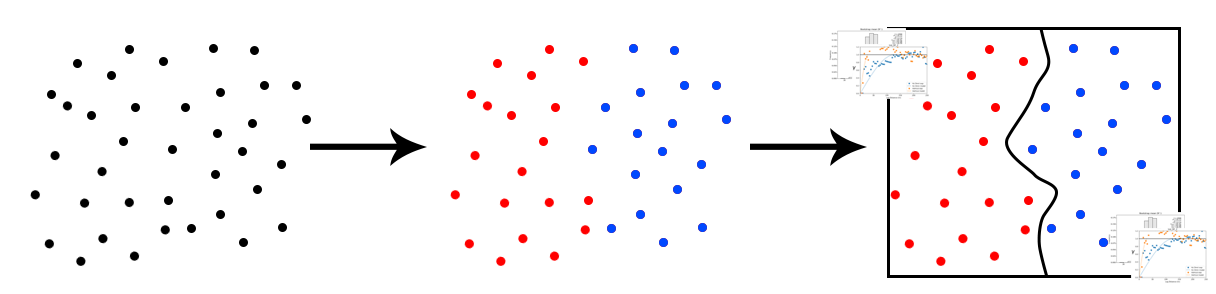
\includegraphics[width=\textwidth]{apresentacao/passo_2}
		\caption{Interpretação e modelagem geológica.}
	\end{center}
\note{Após a coleta, gerenciamento e checagem dos dados, é necessário identificar diferentes domínios. A determinação dos domínios deve ser baseada no conhecimento geológico, como zonas de oxidação, diferentes litologias, alteração ou limites estruturais e deve ser suportada por uma extensiva análise estatística e variográfica e pode ser baseada na combinação de uma ou mais variáveis.
	
	A definição de diferentes domínios é necessária porque a inferência geostatística exige a decisão de estacionariedade. Os teores em cada domínio estacionários pertencem a populações estatística diferentes caracterizadas por seu modelo de distribuição de probabilidades (o histograma) e seu modelo de covariâncias (o variograma).
	
	Uma vez que os domínios tenham sido definidos um modelo tridimensional que define os limites de cada função aleatória estacionária deve ser construído. Esse é o modelo geológico: Ele define a jurisdição espacial de cada função aleatória. O modelo geológico é o alicerce para para todo o trabalho de estimativa subsequente e muitas vezes é o fator de maior importância na estimativa das tonelagens mineralizadas.}
\end{figure}

\end{frame}

\subsection{Método tradicional}

\begin{frame}{Metodologia tradicional}

A abordagem tradicional para a criação de modelos geológicos tridimensionais é através da triangulação de polilinhas.

\begin{figure}[H]
	\begin{center}
		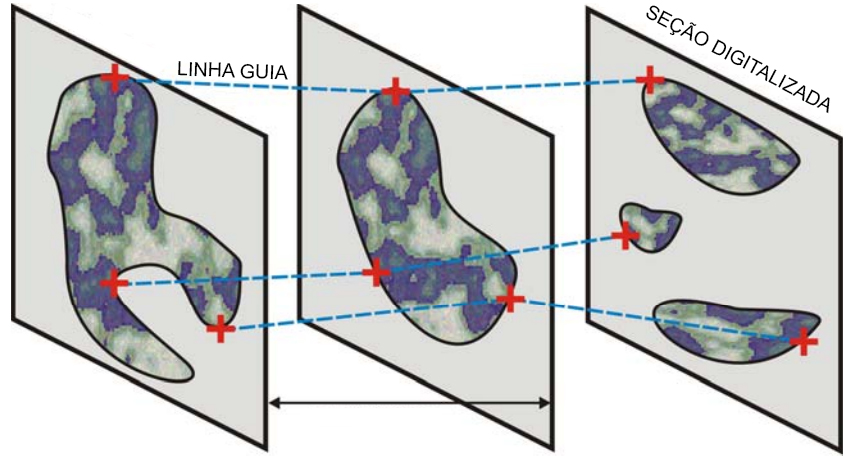
\includegraphics[width=0.6\textwidth]{capitulo_1/explicitmodeling}
		\caption{Esquema do método tradicional.}
	\end{center}
\end{figure}
\note{Tradicionalmente os modelos geológico são construídos de forma explícita: o geomodelador digitaliza manualmente polilinhas em seções verticais e horizontais a partir dos dados de sondagem, as polilinhas são unidas por linhas guias e trianguladas gerando uma representação do sólido geológico.}
\end{frame}

\begin{frame}{Desvantagens do método tradicional}
	\begin{itemize}
		\item Tedioso e demorado;
		\item Exige um profissional especializado e experiente;
		\item Geometria dos corpos precisa ser simplificada;
		\item Subjetivo;
		\item Não replicável;
		\item Inflexível;
		\item Não avalia a incerteza.
	\end{itemize}
\note{Embora a metodologia tradicional seja direta e simples e que softwares de mineração forneçam ferramentas computacionais para agilizar o processo, ainda existem uma série de desvantagens e limitações:
	
	* O processo é tedioso e demorado. Em depósitos de alta complexidade não é raro o geomodelador rabalhar por três meses no modelo geológico.
	
	* Digitaliazar manualmente as polilinhas exige muito tempo de um profissional experiente;
	
	* A geometria dos corpos geolóigcos muitas vezes precisa ser simplificada para que o modelo seja concebido em tempo hábil;
	
	* O processo é subjetivo, Geomodeladores diferentes criam modelos geológicos diferentes a partir do mesmo banco de dados;
	
	* Por esse motivo os modelos geológicos criados a partir do método tradicional não são replicáveis consequentemente não auditáveis;
	
	* O método é inflexível, já que a meidida que novas amostras são obtidas, a atualização do modelo demanda nova gigitalização manual;
	
	* Em muitas minas, talvez na grande maioria delas, apenas um modelo geológico é construído e mantido por questões de tempo. Assim não há a oportunidade de modelar interpretações geológicas alterantivas e comparar estimavas de recursos baseadas em diferentes modelos. Além da redigitalização manual não existe forma direta de incorporar múltiplas realizações possíveis para a localização dos limites entre os diferentes domínios no método tradicional.}
\end{frame}

\subsection{Incerteza do modelo geológico}

\begin{frame}{Incerteza do modelo geológico}

Em muitos casos, a incerteza do modelo geológico pode ser uma fonte de incerteza crucial e deve ser avaliada.

\begin{figure}[H]
	\begin{center}
		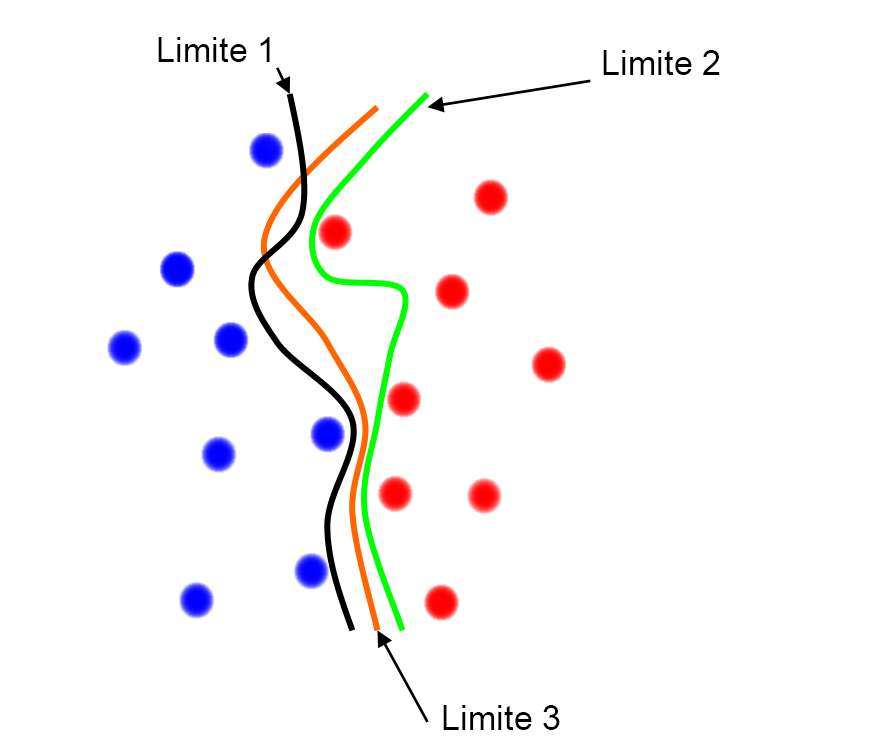
\includegraphics[width=0.4\textwidth]{capitulo_1/incerteza_limites}
		\caption{Incerteza do modelo geológico.}
	\end{center}
\end{figure}
\note{No interior dos domínios não existe incerteza relacionada ao modelo geoógico, No esquema do slide azul é azul e vermelho é vermelho, a incerteza é associada ao limite que separa os diferentes domínios. Sua definição, em sub superfície, é um mero palpite.
	
	Em muitos casos a incerteza do modelo geológico pode ser uma fonte de incerteza crucial. Em depósitos de veio de ouro por exemplo, o volume mineralizado é um indicador economico vital do projeto e está diretamente ligado ao modelo geológico, ignorar a incerteza do modelo geológico pode ser devastador para o empredimento. A incerteza do modelo geológico DEVE ser avaliada. }
\end{frame}

\subsection{Métodos matemáticos}

\begin{frame}{Métodos matemáticos}

	\begin{columns}[t]
		\begin{column}{0.5\textwidth}
			\begin{center}
				\textit{Métodos determinísticos}
			\end{center}
			\begin{itemize}
				\item Vizinho mais próximo;
				\item Krigagem dos indicadores.
			\end{itemize}
		\end{column}
		\begin{column}{0.5\textwidth}
			\begin{center}
				\textit{Métodos estocásticos}
			\end{center}
			\begin{itemize}
				\item Simulação sequencial dos indicadores;
				\item Simulação gaussiana/plurigaussiana truncada;
				\item Simulação multi ponto;
				\item Simulação baseada em objetos;
			\end{itemize}
		\end{column}
	\end{columns}
	\note{As desvantagens do método explícito impulsionaram a criação de métodos automáticos, ou pelo menos semi automáticos, de modelagem geológica. Para a criação de modelos determinísticos, podem ser utilizados desde métodos matemáticos mais simples como o vizinho mais próximo, como geostatísticos como a krigagem dos indicadores. 
		
		Já a necessidade de avaliação da incerteza impulsionou o desenvolvimento de métodos estocásticos, baseados em múltiplas realizações equiprováveis do modelo geológico. Metodologias estabelecidas da geostatística clássica, baseadas no variograma, são a simulação sequencial dos indicadores, simulação gaussiana truncada e siulação plurigaussiana truncada. Outros métodos não baseados no variograma também foram desenvolvidos: simulação multi ponto, simulação baseada em objetos são os principais expoentes. }
\end{frame}

\subsection{Métodos implícitos}

\begin{frame}{Métodos implícitos}
	\begin{figure}[H]
		\begin{center}
			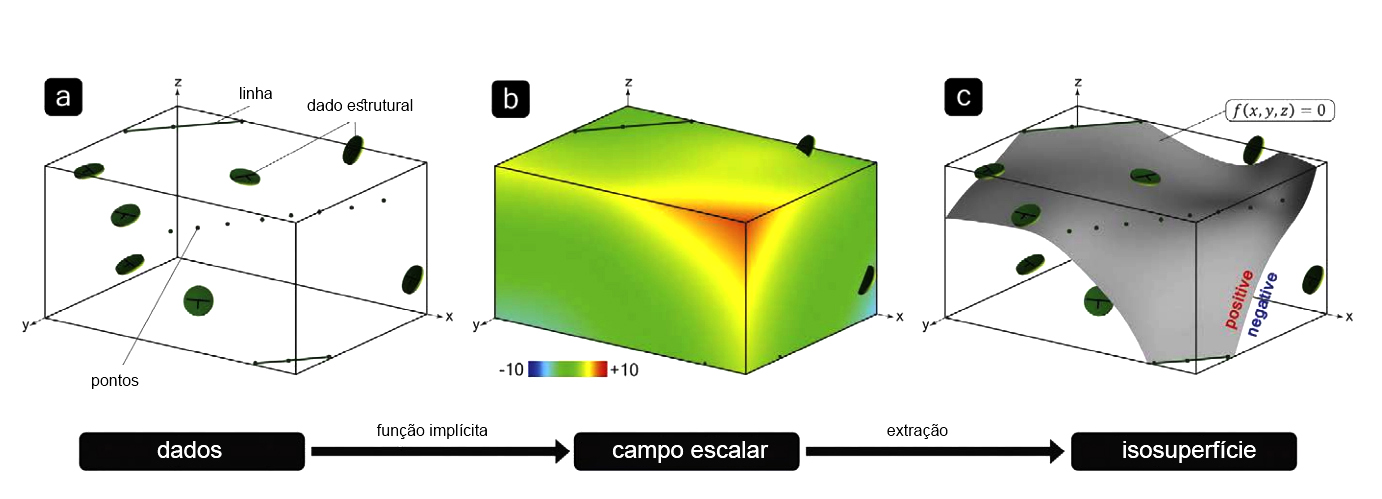
\includegraphics[width=0.8\textwidth]{capitulo_1/implicit_modelig_pt_1}
			\caption{Esquema dos métodos implícitos.}
		\end{center}
	\end{figure}

\begin{itemize}
	\item \cite{mallet2004space} propõe uma função volumétrica cronológica, levando em consideração a posição estratigráfica das diferentes unidades geológicas;
	\item \cite{lajaunie1997foliation} usam co-krigagem de incrementos em um campo potencial, omitindo a função volume.
\end{itemize}
\note{Uma outra família de métodos que impotaram técnicas da computação gráfica são os métodos implícitos. A idéia central é usar uma função implícita para demarcar regiões no espaço. 
	
	Todos os métodos implícitos compartilham da mesma mecânica. A partir de dados esparsos que podem ser categorias, dados estruturais, podem ser em pontos ou linhas... Uma função implícita é derivada, o campo escalar, que têm um número infinito de isosuperfícies. Para visualizar o modelo geológico uma isosuperfície expecífica deve ser extraída desse modelo implícito, geralmente a isosuperfície 0.
	
	O que difere os métodos implícitos é a função volume, que é interpolada para criação do modelo implícito. mallet propôs uma função volume cronológica, baseada na posição estratigráfica das unidades geológicas. Um outro método implícito, nascido na escola de minas da frança, usa co-krigagem de incrementos em campo potencial omitindo a função volume.
	
	De longe a função volume mais comum é a função distância assinalada, aplicações desse método são encontradas por toda a literatura de interpolação de dados esparços. Na modelagem geológica o método é competente em capturar a geometria e extensão de corpos geológicos e tem sido aplicada com sucesso há mais de 10 anos na exploração mineral. Nos últimos anos vem ganhado espaço em diversos softwares comerciais o maior exemplo é o leapfrog. }
\end{frame}


\section{Modelagem geológica implícita com funções distância assinaladas}

\subsection{O banco de dados}

\begin{frame}{O banco de dados}

72 furos totalizando 3349 amostras distribuídas entre 3 diferentes categorias.

	\begin{figure}
		\centering
		\subfloat[Proporções.]{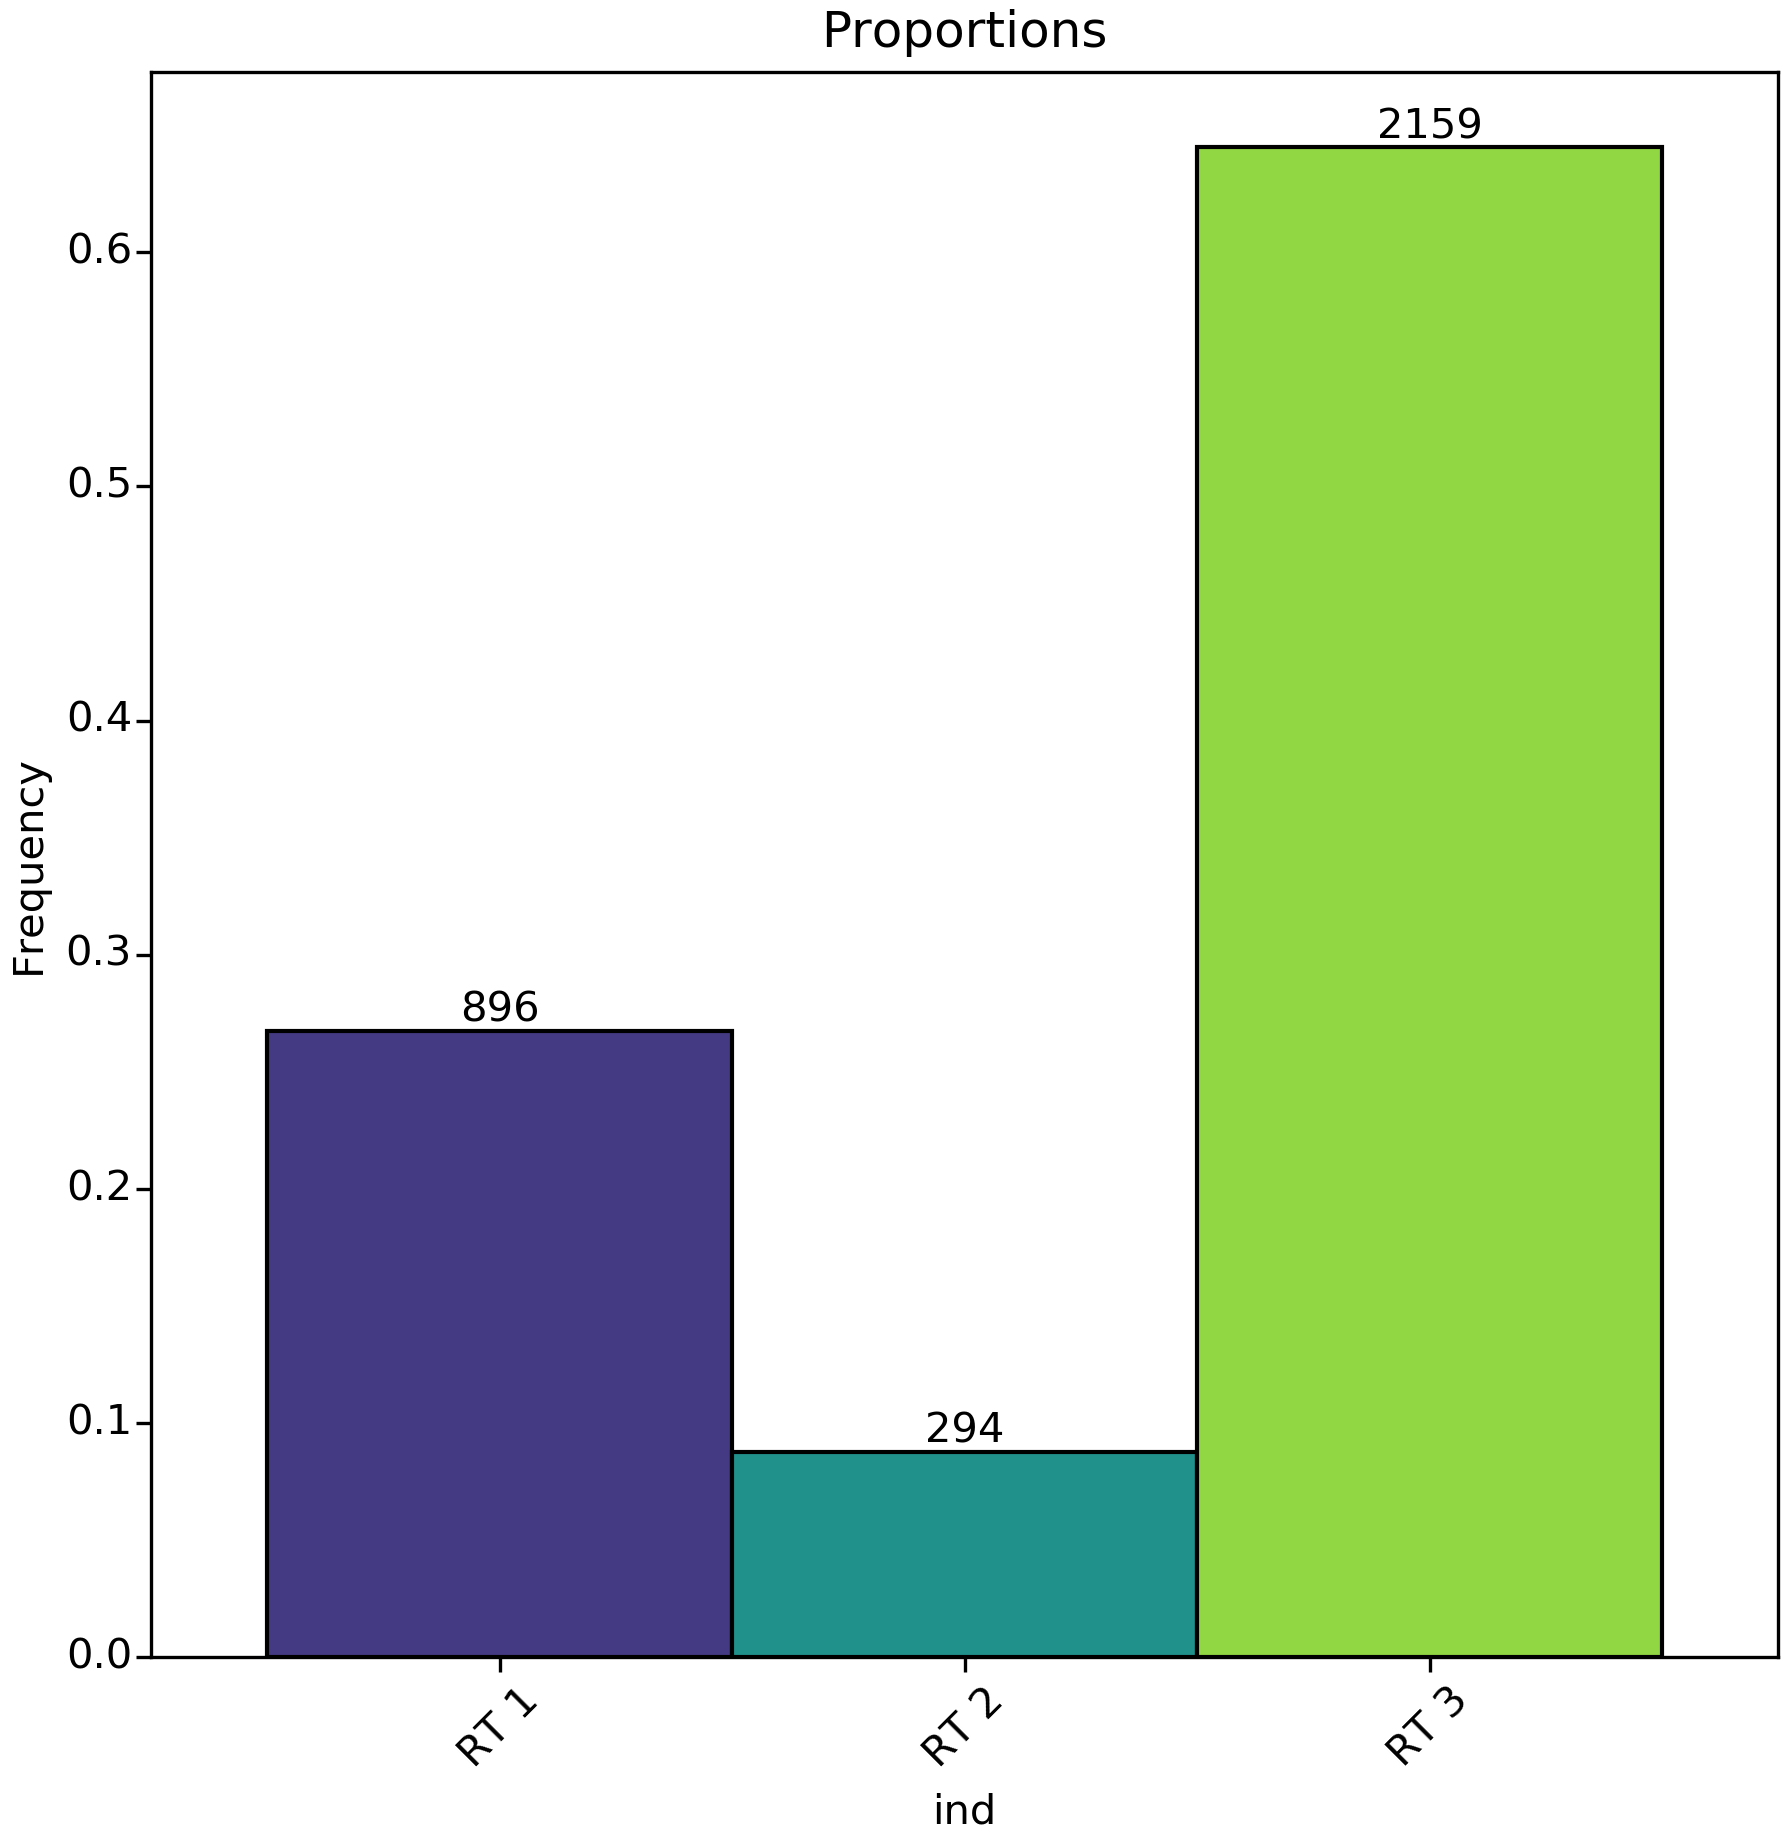
\includegraphics[width=.25\textwidth]{capitulo_2/prop_hist_big.png}}\hspace{20mm}
		\subfloat[Vista das amostras.]{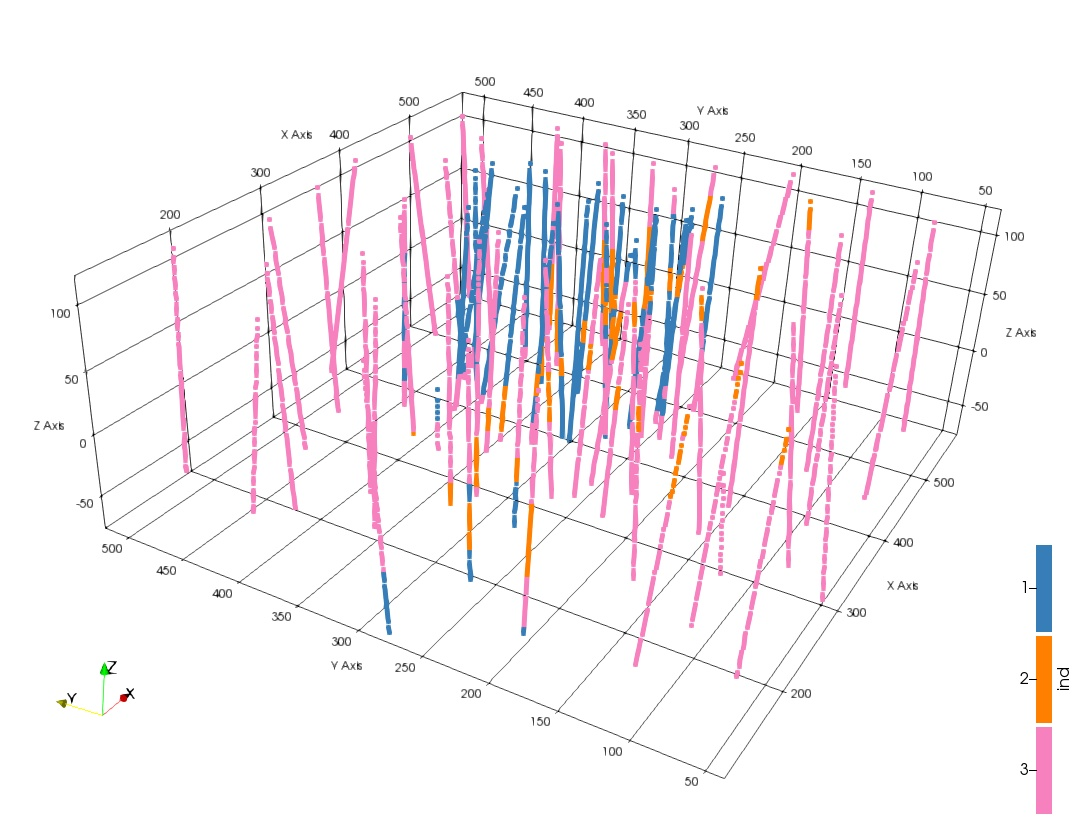
\includegraphics[width=.4\textwidth]{capitulo_2/dados.jpeg}}
		\caption{O banco de dados.}
	\end{figure}
		\note{Nos próximos slides a modelagem geológica implícita com distâncias assinaladas é explicada passo a passo e os métodos para avaliação de inceteza disponíveis na literatura são apresentadas. 
			
			Um banco de dados sintético que emula um depósito de cobre pórfiro é usado para exemplificar e comparar os métodos. São 72 furos, totalizando cerca de 3 mil amostras, distribuídas entre três categorias: uma rocha encaixante e duas intrusões: uma vertical e uma tabular com mergulho. O slide mostra as proprções de cada litologia e uma vista em perspectiva das amostras.}
\end{frame}

\subsection{Codificando as amostras em indicadores}

\begin{frame}{Codificando as amostras em indicadores}
	\begin{equation}
	i_k(u_\alpha)=\begin{cases}
	1,\:\textrm{se}\:z(u_\alpha)\:\textrm{se pertence ao domínio $k$}\\
	0,\:\textrm{se}\:z(u_\alpha)\:\textrm{caso contrário}\end{cases}
	\label{eq_ind}
	\end{equation}
	
	\begin{figure}[H]
		\caption{Amostras codificadas em indicadores para cada uma das três categorias do banco de dados.} \label{ind}
		\centering
		\subfloat[][Categoria 1]{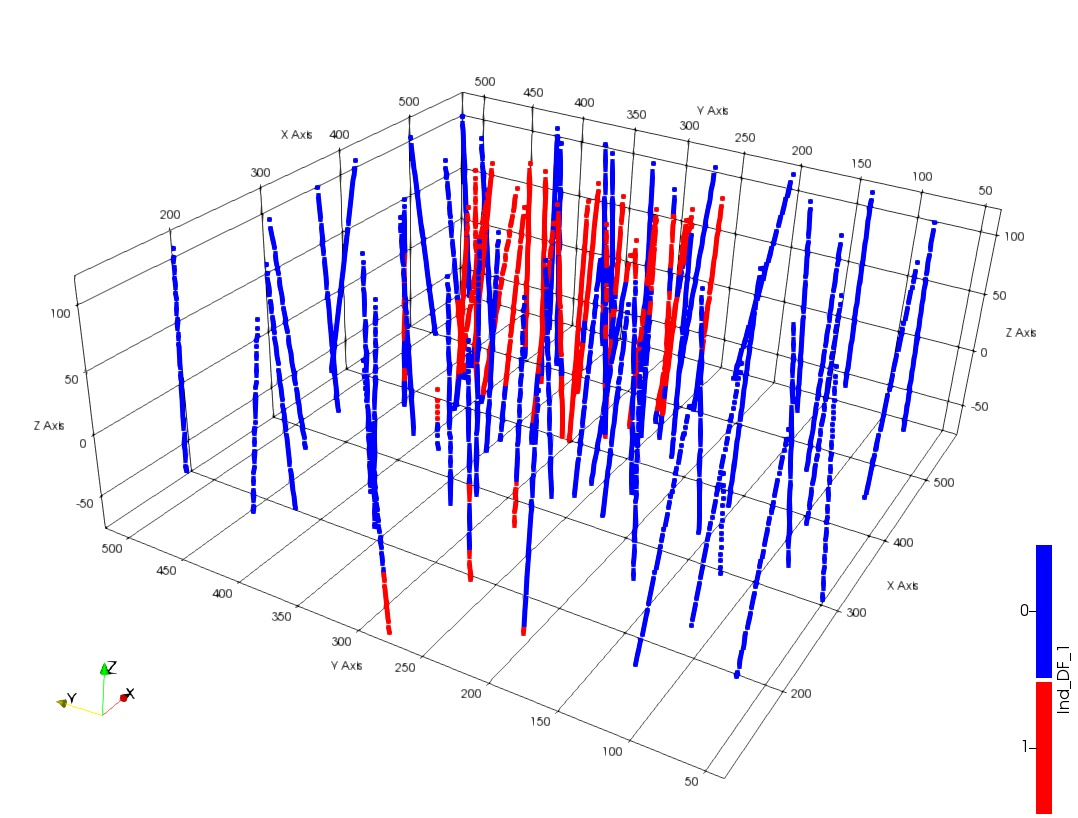
\includegraphics[width=.3\textwidth]{capitulo_2/inddf1.jpeg}\label{<figure1>}}
		\subfloat[][Categoria 2]{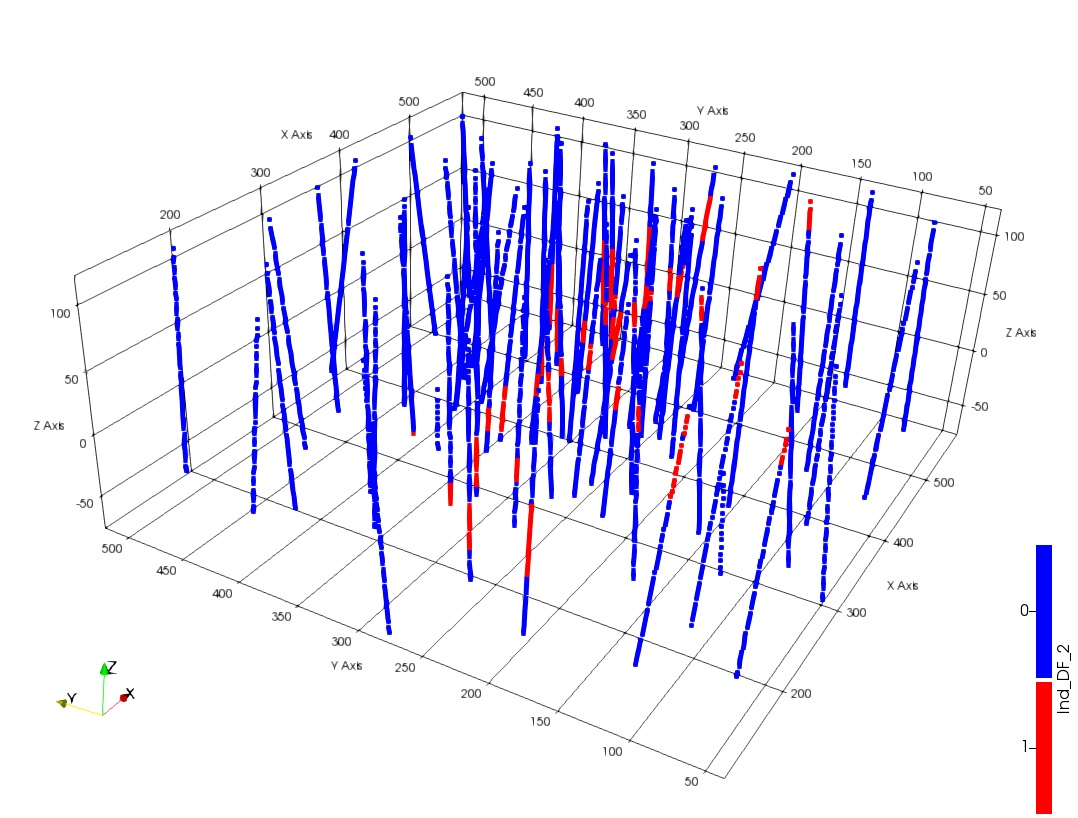
\includegraphics[width=.3\textwidth]{capitulo_2/inddf2.jpeg}\label{<figure2>}}
		\subfloat[][Categoria 3]{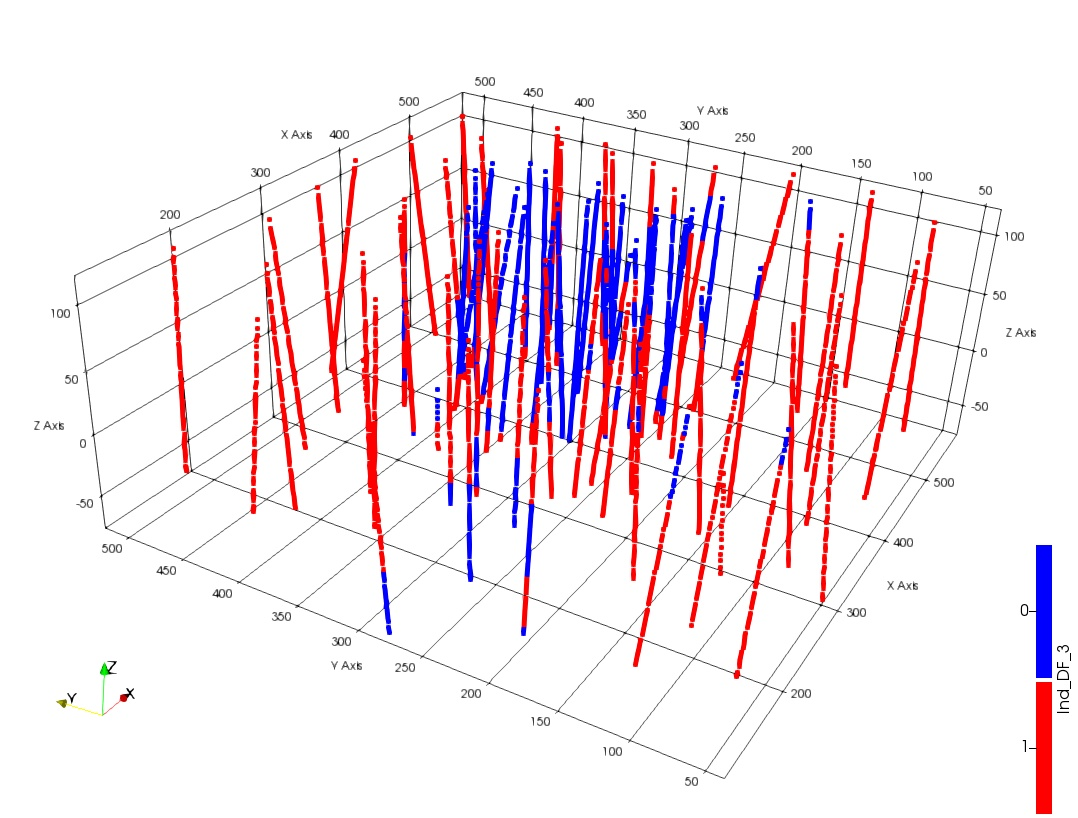
\includegraphics[width=.3\textwidth]{capitulo_2/inddf3.jpeg}\label{<figure2>}}
	\end{figure}
\note{O primeiro passo é codificar as amostras em indicadores: uma amostra recebe o indicador 1 se pertencer ao domínio que está sendo modelado e 0 caso contrário. O slide mostra as amostras codificadas em indicadores para as categorias 1, 2 e 3.}
\end{frame}

\subsection{Calculando a função distância assinalada}

\begin{frame}{Calculando a função distância assinalada}

\begin{equation}
d_k(u_\alpha)=\begin{cases}
-\parallel u_\alpha-u_\beta\parallel,\:\textrm{se $u_\alpha$ pertence ao domínio}\\
+\parallel u_\alpha-u_\beta\parallel,\:\textrm{se $u_\alpha$ não pertence ao domínio}\end{cases}
\label{eq_mult_sg}
\end{equation}

O local $u_\beta$ corresponde à amostra mais próxima codificada com um indicador diferente de $u_\alpha$.
\begin{figure}[H]
	\caption{\label{2d_ex}Ilustração esquemática mostrando o cálculo das distâncias assinaladas.}
	\begin{center}
		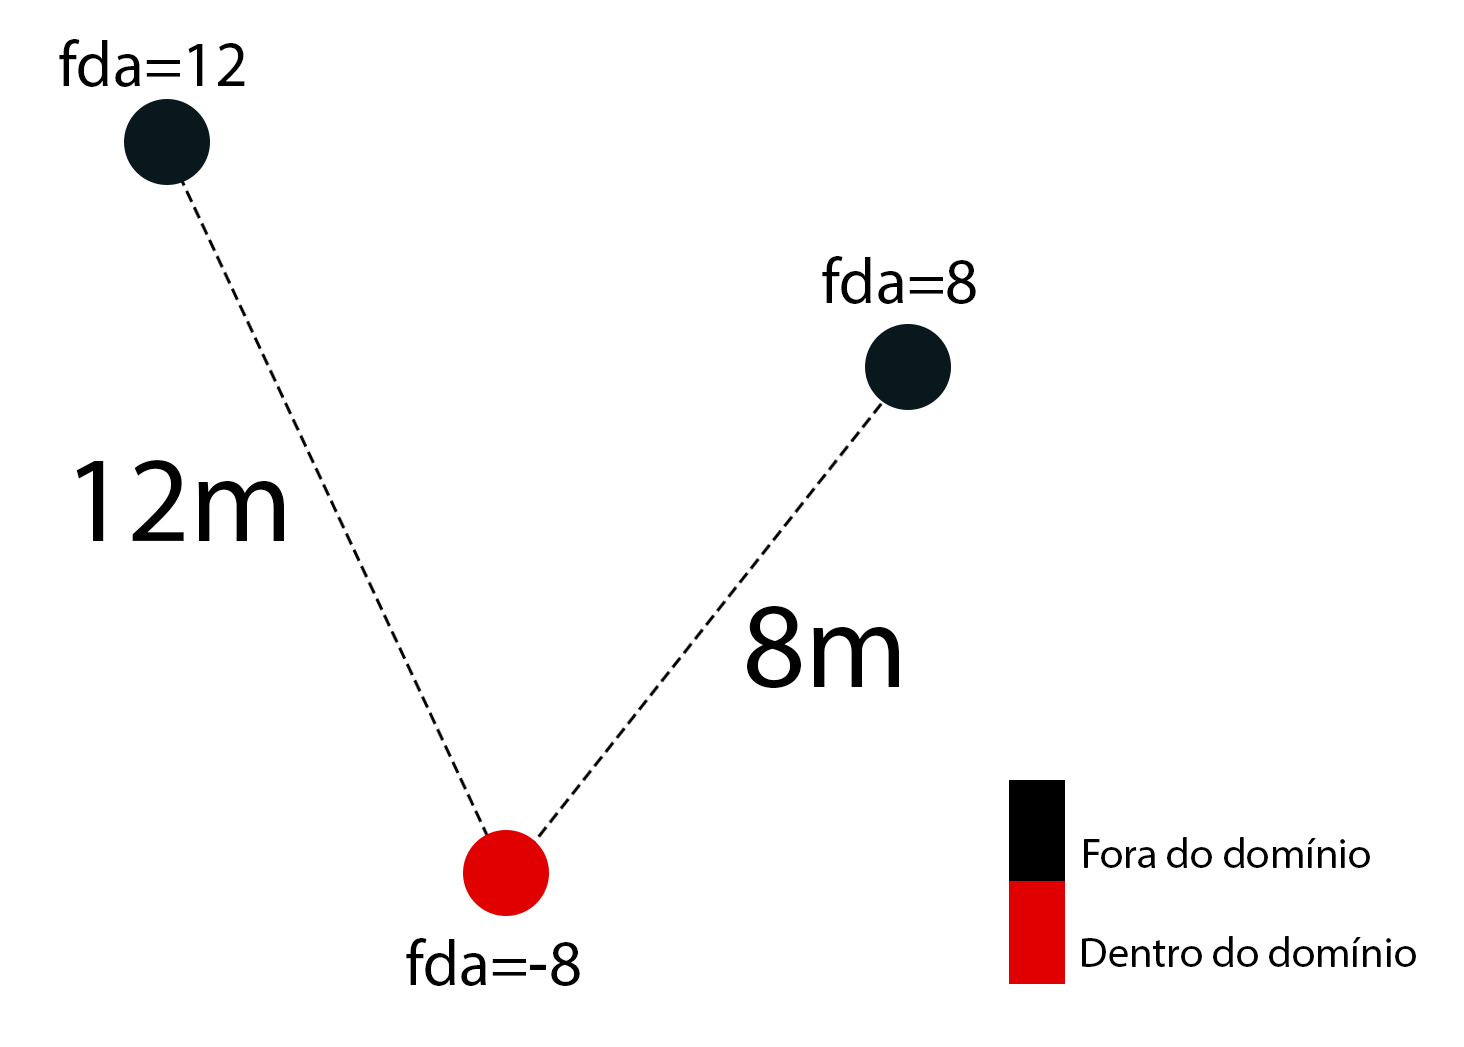
\includegraphics[width=0.3\textwidth]{capitulo_2/2d_ex.jpg}
	\end{center}
	%\legend{Modificado de \citeonline{martin2017implicitmodeling}}
\end{figure}
\note{O segundo passo é o cáculo das distâncias assinaladas: para cada ponto amostral, a menor distância euclideana até um outro ponto amostal que pertença à um indicador oposto é computada e atribuída aquele ponto. Com o sinal negativo caso pertença ao domínio que está sendo modelado e com o sinal positivo caso contrário.
	
	Para o esquema do slide: pra essa amostra preta aqui em cima, ela não pertence ao domínio, então foi codificada com o indicador 0, eu vou computar então a menor distância entre ela e uma outra amostra codificada com o indicador oposto, uma amostra vermelha, que pertence ao domínio. são 12 metros, então essa amostra preta vai receber o valor 12 metros com o sinal positivo, porque não pertence ao domínio. Para a amostra vermelha, vou computar a menor ditância até uma amostra preta, que é essa daqui, 8 metros, então ela recebe 8 metros com o sinal negativo porque pertence ao domínio que está sendo modelado. E finalmente a ultima amostra preta está a 8 metros da vermelha, recebe 8 com o sinal positivo, porque está fora do domínio modelado.}
\end{frame}

\begin{frame}{Calculando a função distância assinalada} 
	\begin{figure}[H]
		\caption{Distâncias assinaladas calculadas para cada uma das categorias do banco de dados.} \label{indcalc}
		\centering
		\subfloat[][Categoria 1]{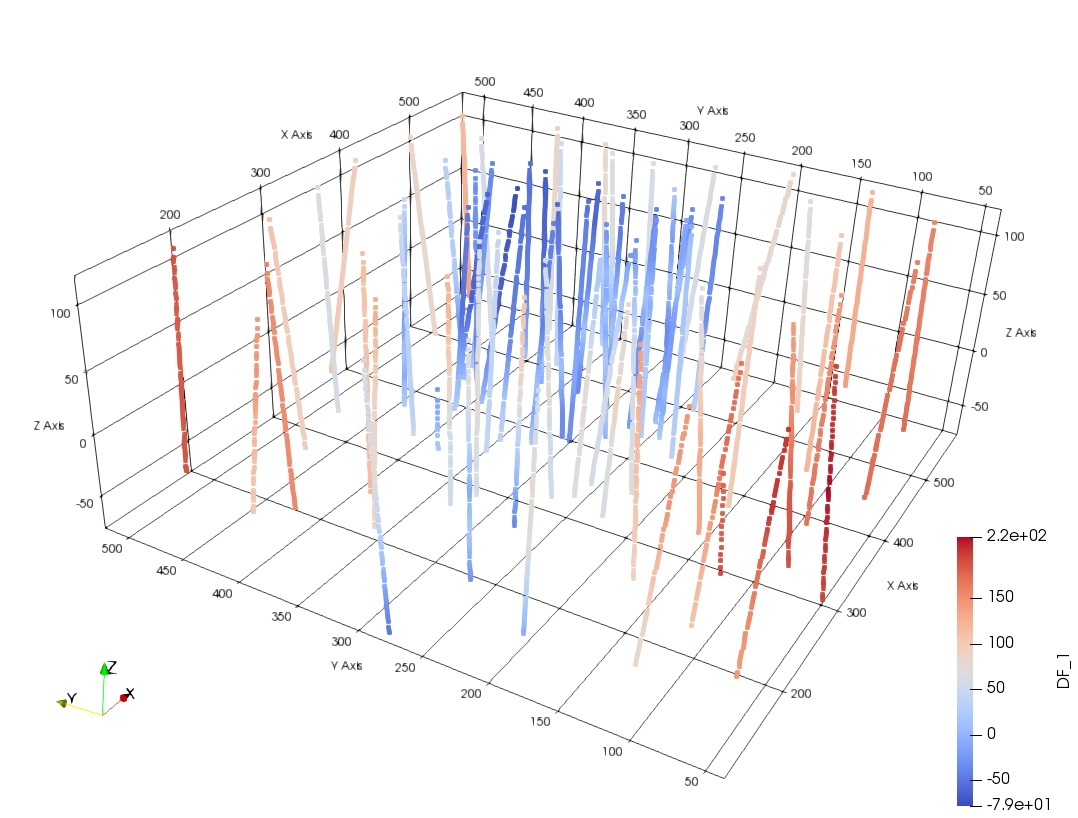
\includegraphics[width=.3\textwidth]{capitulo_2/df1.jpeg}\label{<figure1>}}
		\subfloat[][Categoria 2]{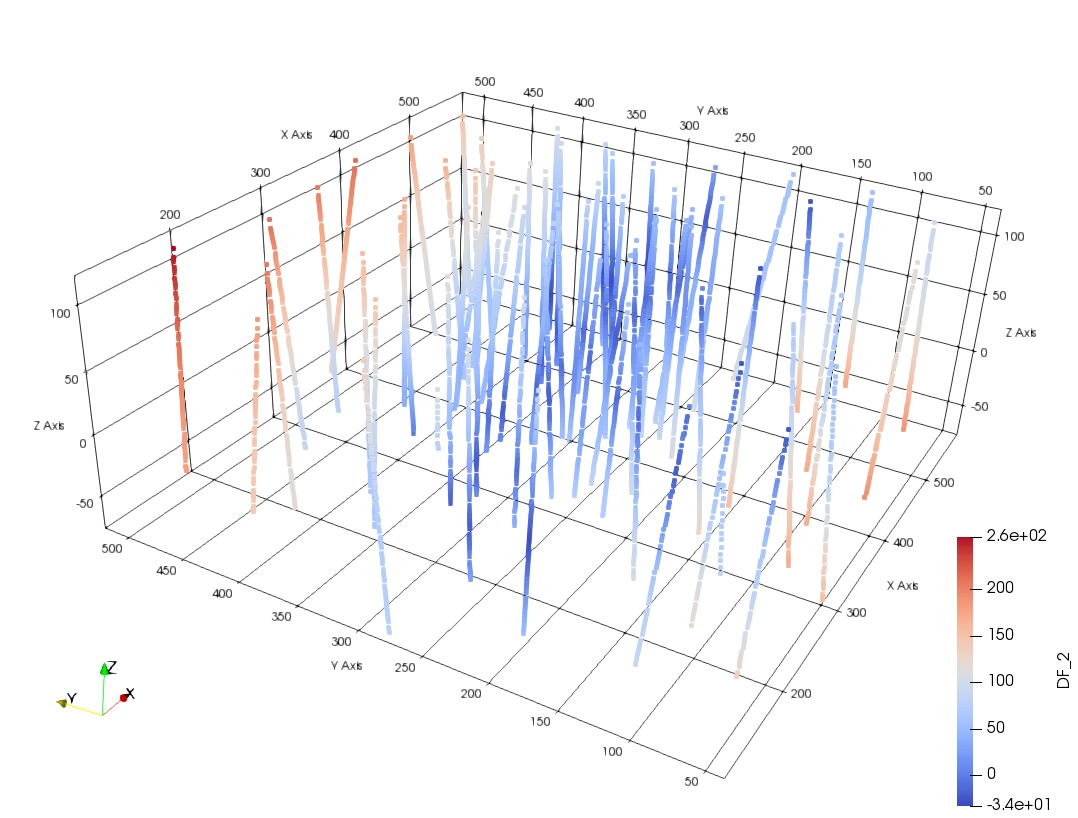
\includegraphics[width=.3\textwidth]{capitulo_2/df2.jpeg}\label{<figure2>}}
		\subfloat[][Categoria 3]{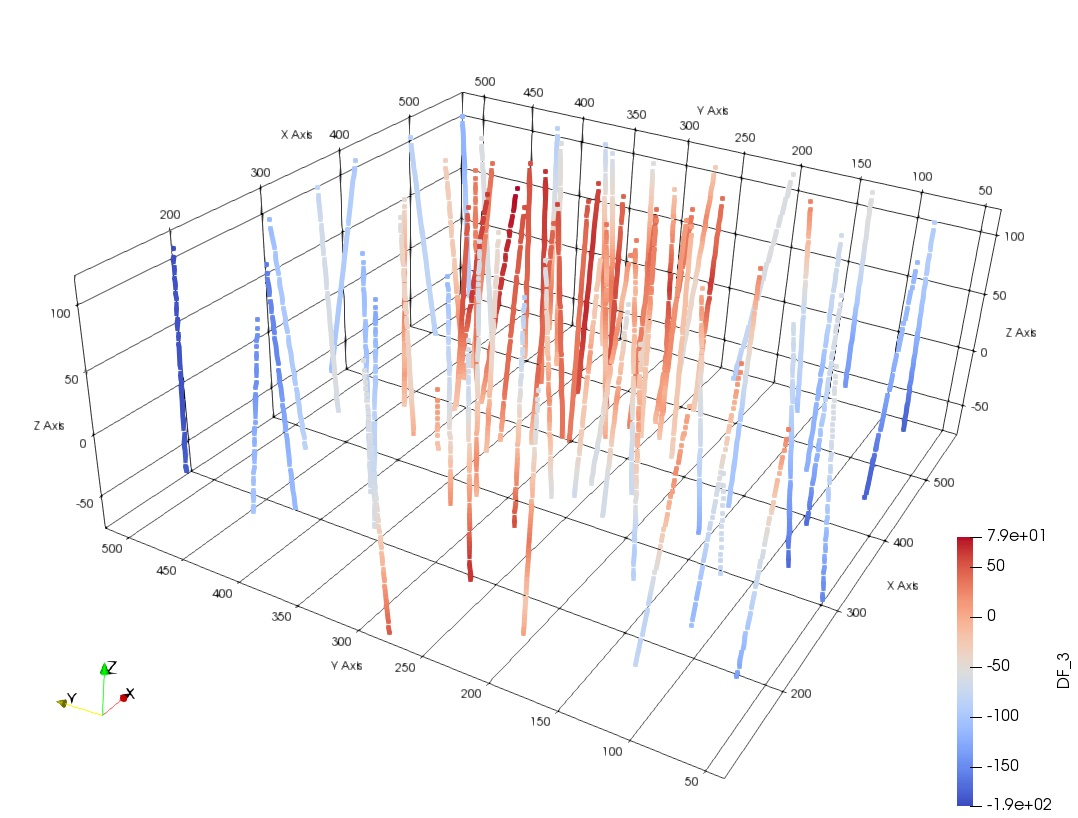
\includegraphics[width=.3\textwidth]{capitulo_2/df3.jpeg}\label{<figure2>}}
	\end{figure}
\note{Esse slide mostra as distâncias assinaladas calculadas para as litologias 1, 2 e 3.
}
\end{frame}

\subsection{Variografia das distâncias assinaladas}

\begin{frame}{Variografia das distâncias assinaladas}

Distâncias assinaladas não são estacionárias, o variograma não se estabiliza em um patamar. Além disso, o caráter extremamente contínuo das distâncias torna a identificação analítica das direções principais um processo embaraçoso.

\begin{itemize}
	\item Treinar o variograma usando validação cruzada;
	\item Tentar modelar interativamente os variogramas experimentais;
	\item Calcular e modelar os variogramas para as propriedades de indicadores e transformá-los em um equivalente gaussiano para as distâncias assinaladas;
	\item inferir um modelo de covariância plausível visualmente a partir das amostras ou de mapas delineados a mão.
\end{itemize}
\note{Agora as distâncias calculadas precisam ser interpoladas, alguns dos métodos de interpolação, que eu vou detalhar daqui a pouco, exigem uma função de covariância, que pode ser obtida a partir dos dados.
	
	Aqui surge o primeiro problema do método: as distâncias assinaladas não são estacionárias, isso quer dizer que o variograma não se estabiliza em um patamar, ele cresce indefinidamente à medida que o lag aumenta, dificultando a inferência do alcance. Além disso, as distâncias apresentam um comportamento extremamaente contínuo, que torna difícil a indentificação de direções principais. Esse caráter contínuo das distâncias faz com que o modelo gaussiano seja o mais indicado pra ajustar os variogramas.
	
	A literatura sugere alternativas:
	
	* Treinar o variograma usando validação cruzada;
	
	* Tentar modelar de fato os variogramas experimtnais;
	
	* Calcular e modelar o variograma dos indicadores e transformá-los em um equivalente gaussiano;
	
	* Inferir um modelo de covariância plausível visualmente, a partir das amostras ou mapas delineados.}
\end{frame}

\begin{frame}{Variogramas das distâncias assinaladas}
\begin{figure}[H] 
	\caption{Variogramas experimentais das distâncias assinaladas e modelos para cada uma das categorias do banco de dados.} \label{sd_var}
	\centering
	\subfloat[][Categoria 1]{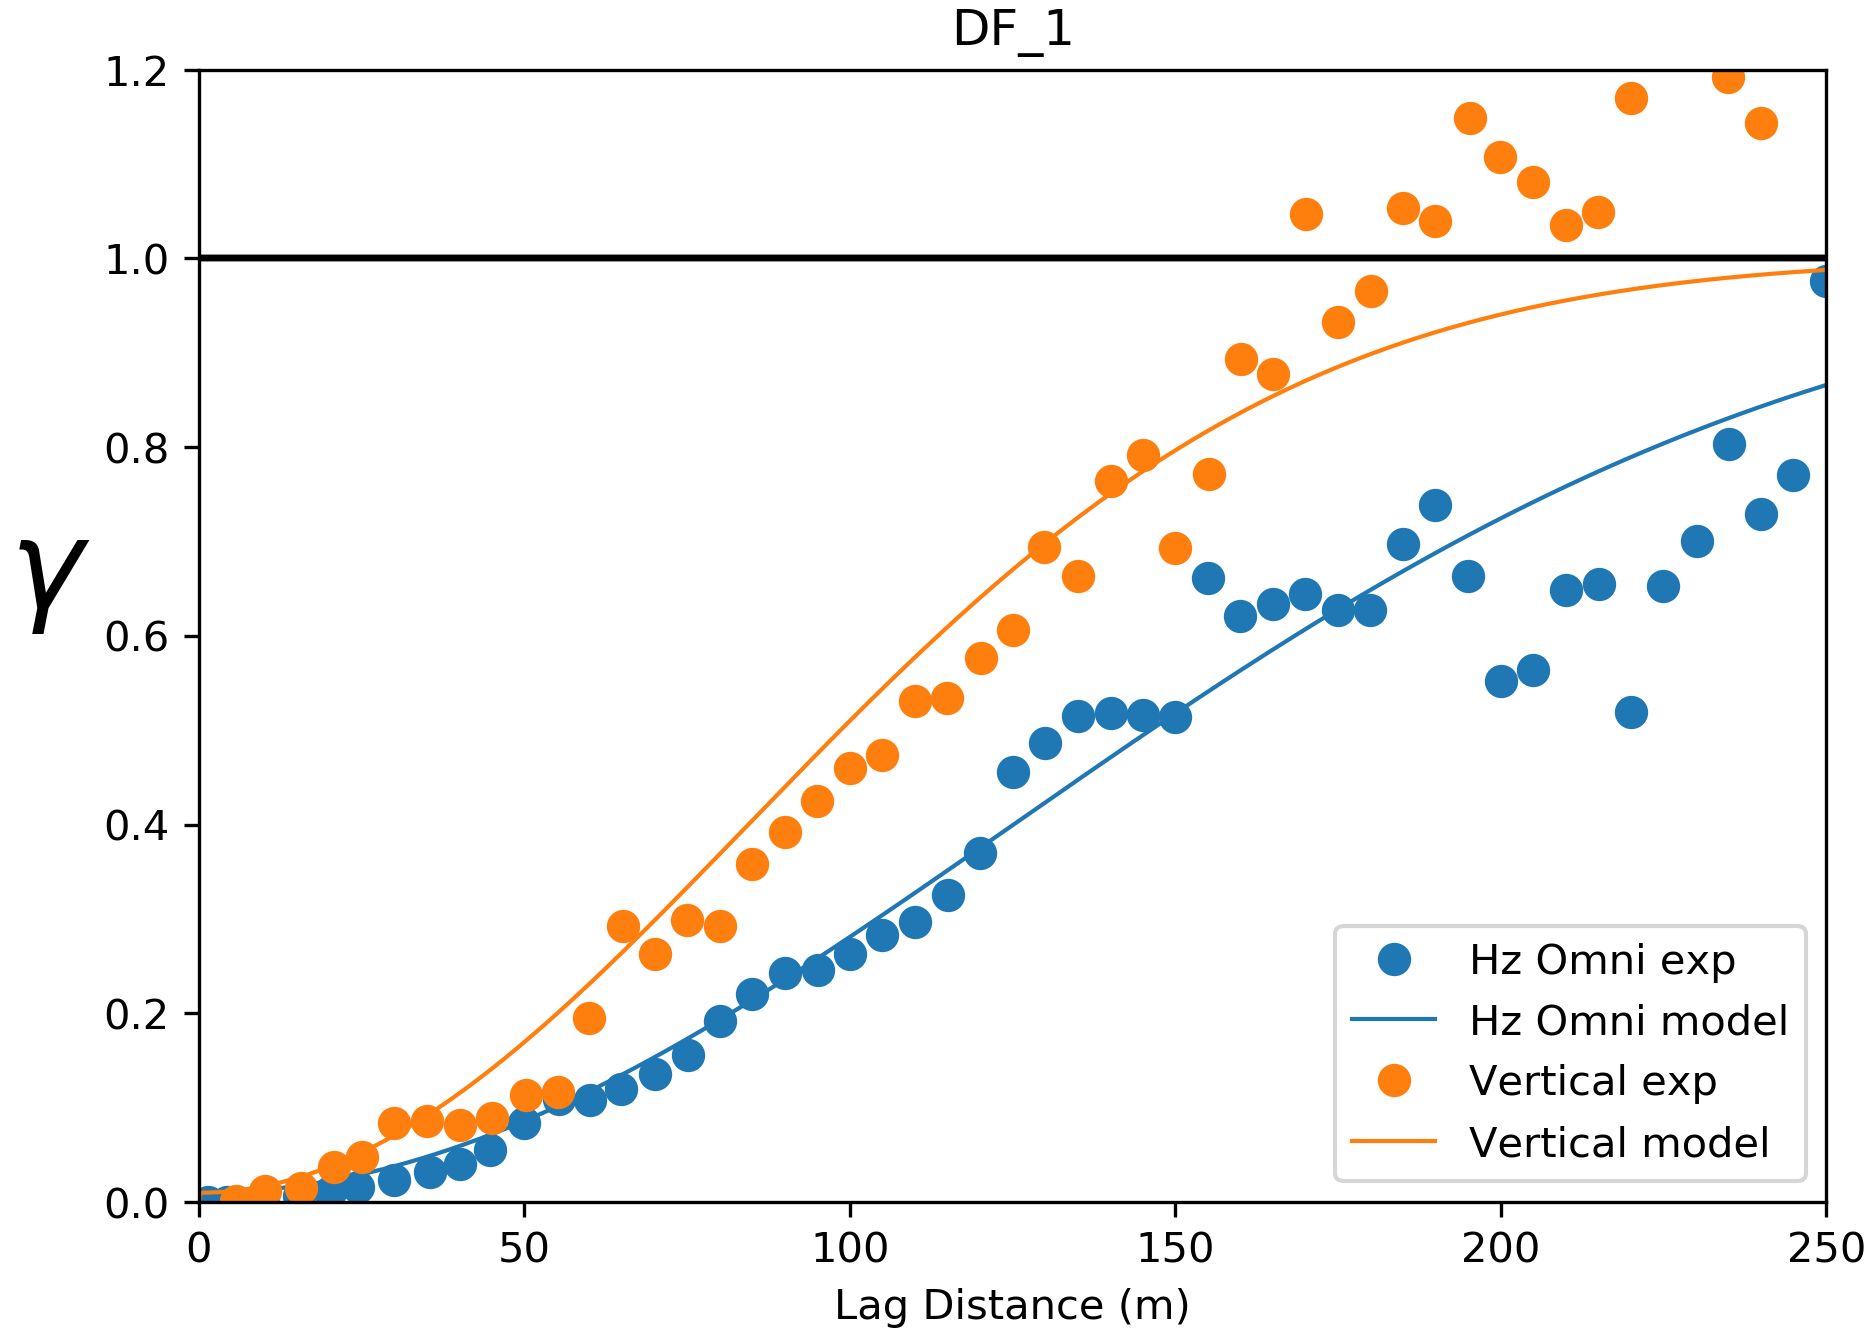
\includegraphics[width=.3\textwidth]{capitulo_2/var_DF_1.png}\label{<figure1>}}
	\subfloat[][Categoria 2]{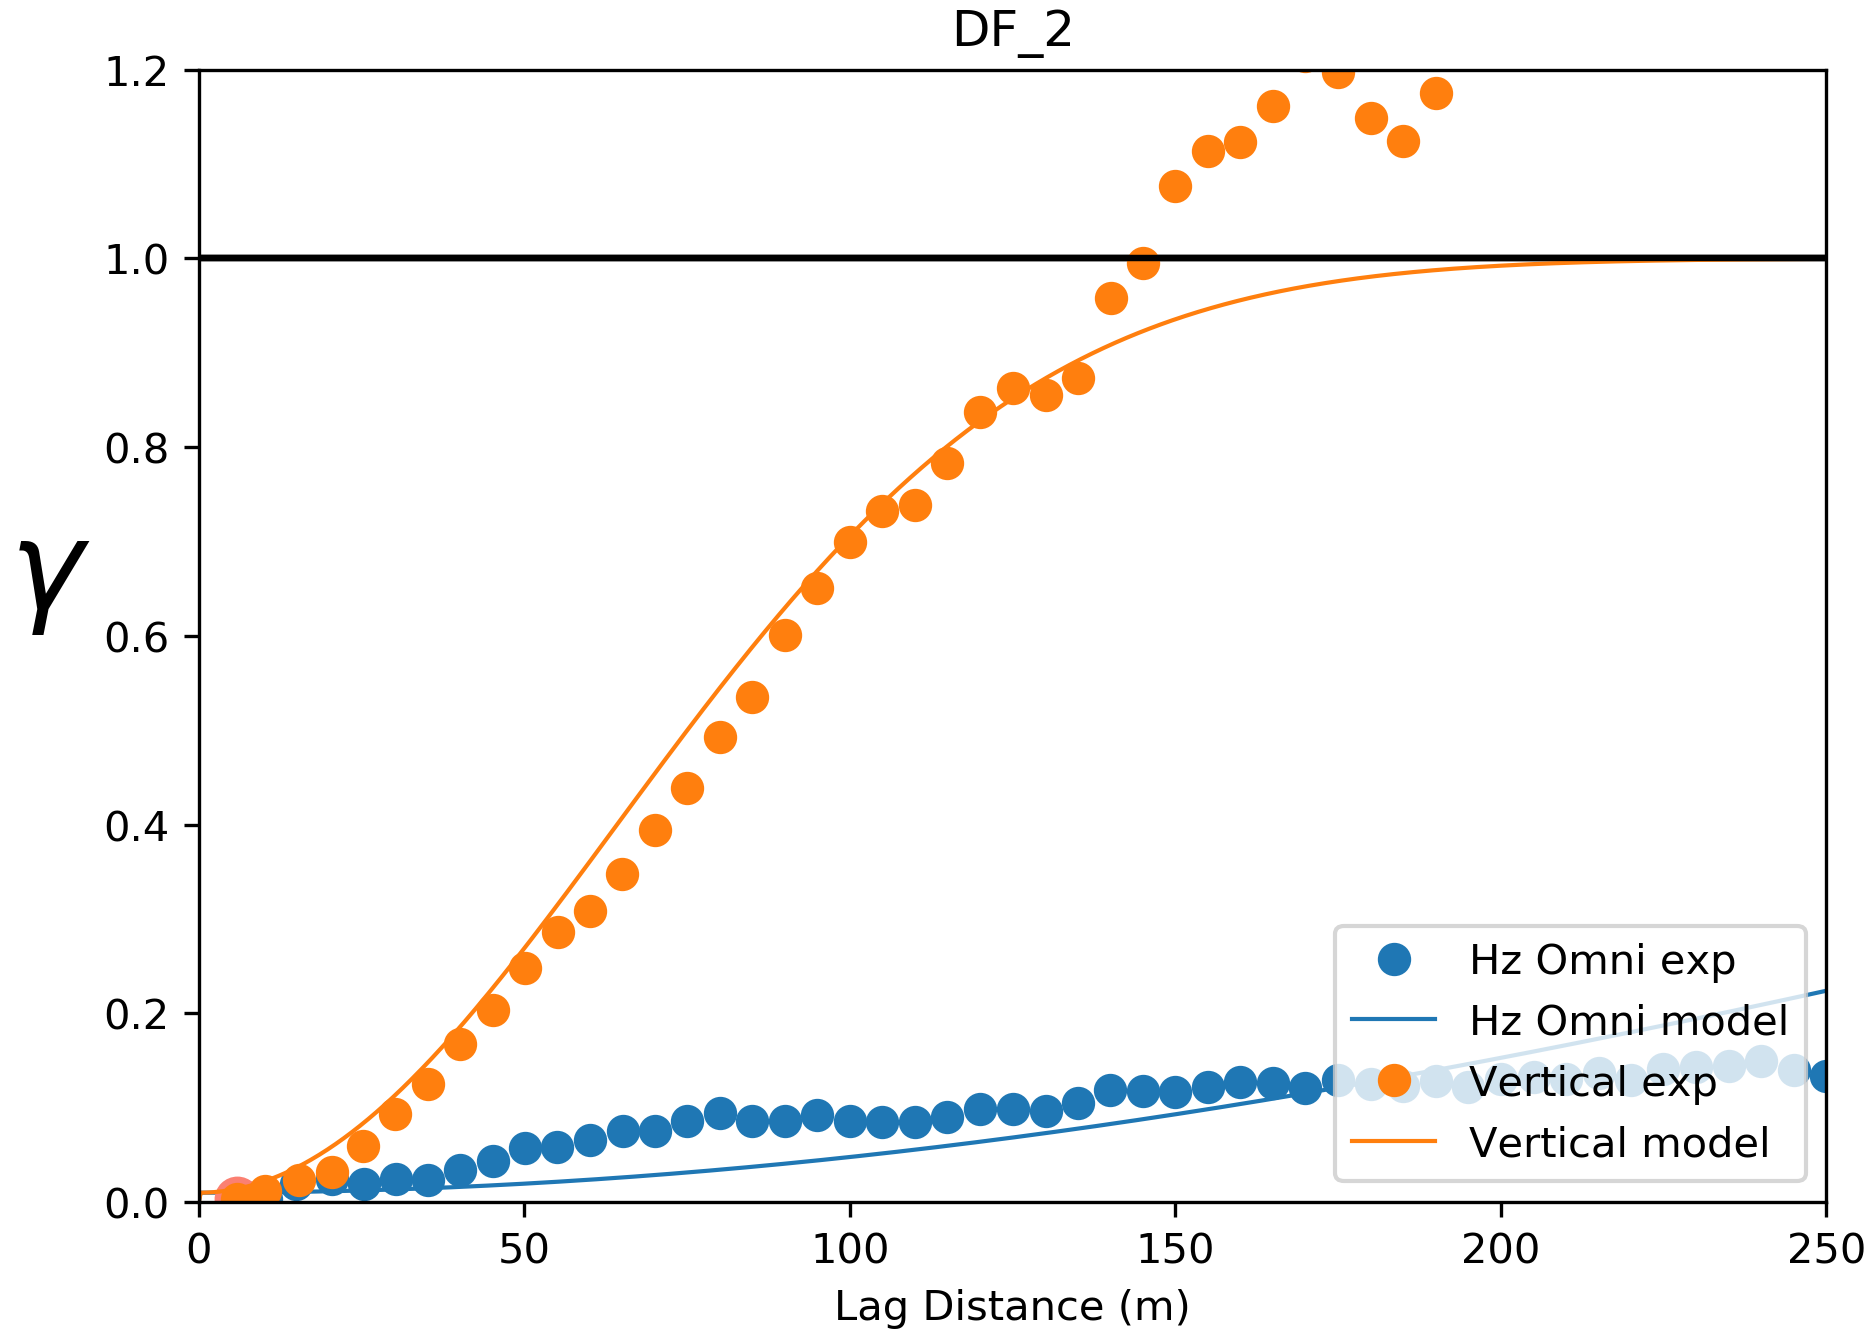
\includegraphics[width=.3\textwidth]{capitulo_2/var_DF_2.png}\label{<figure2>}}
	\subfloat[][Categoria 3]{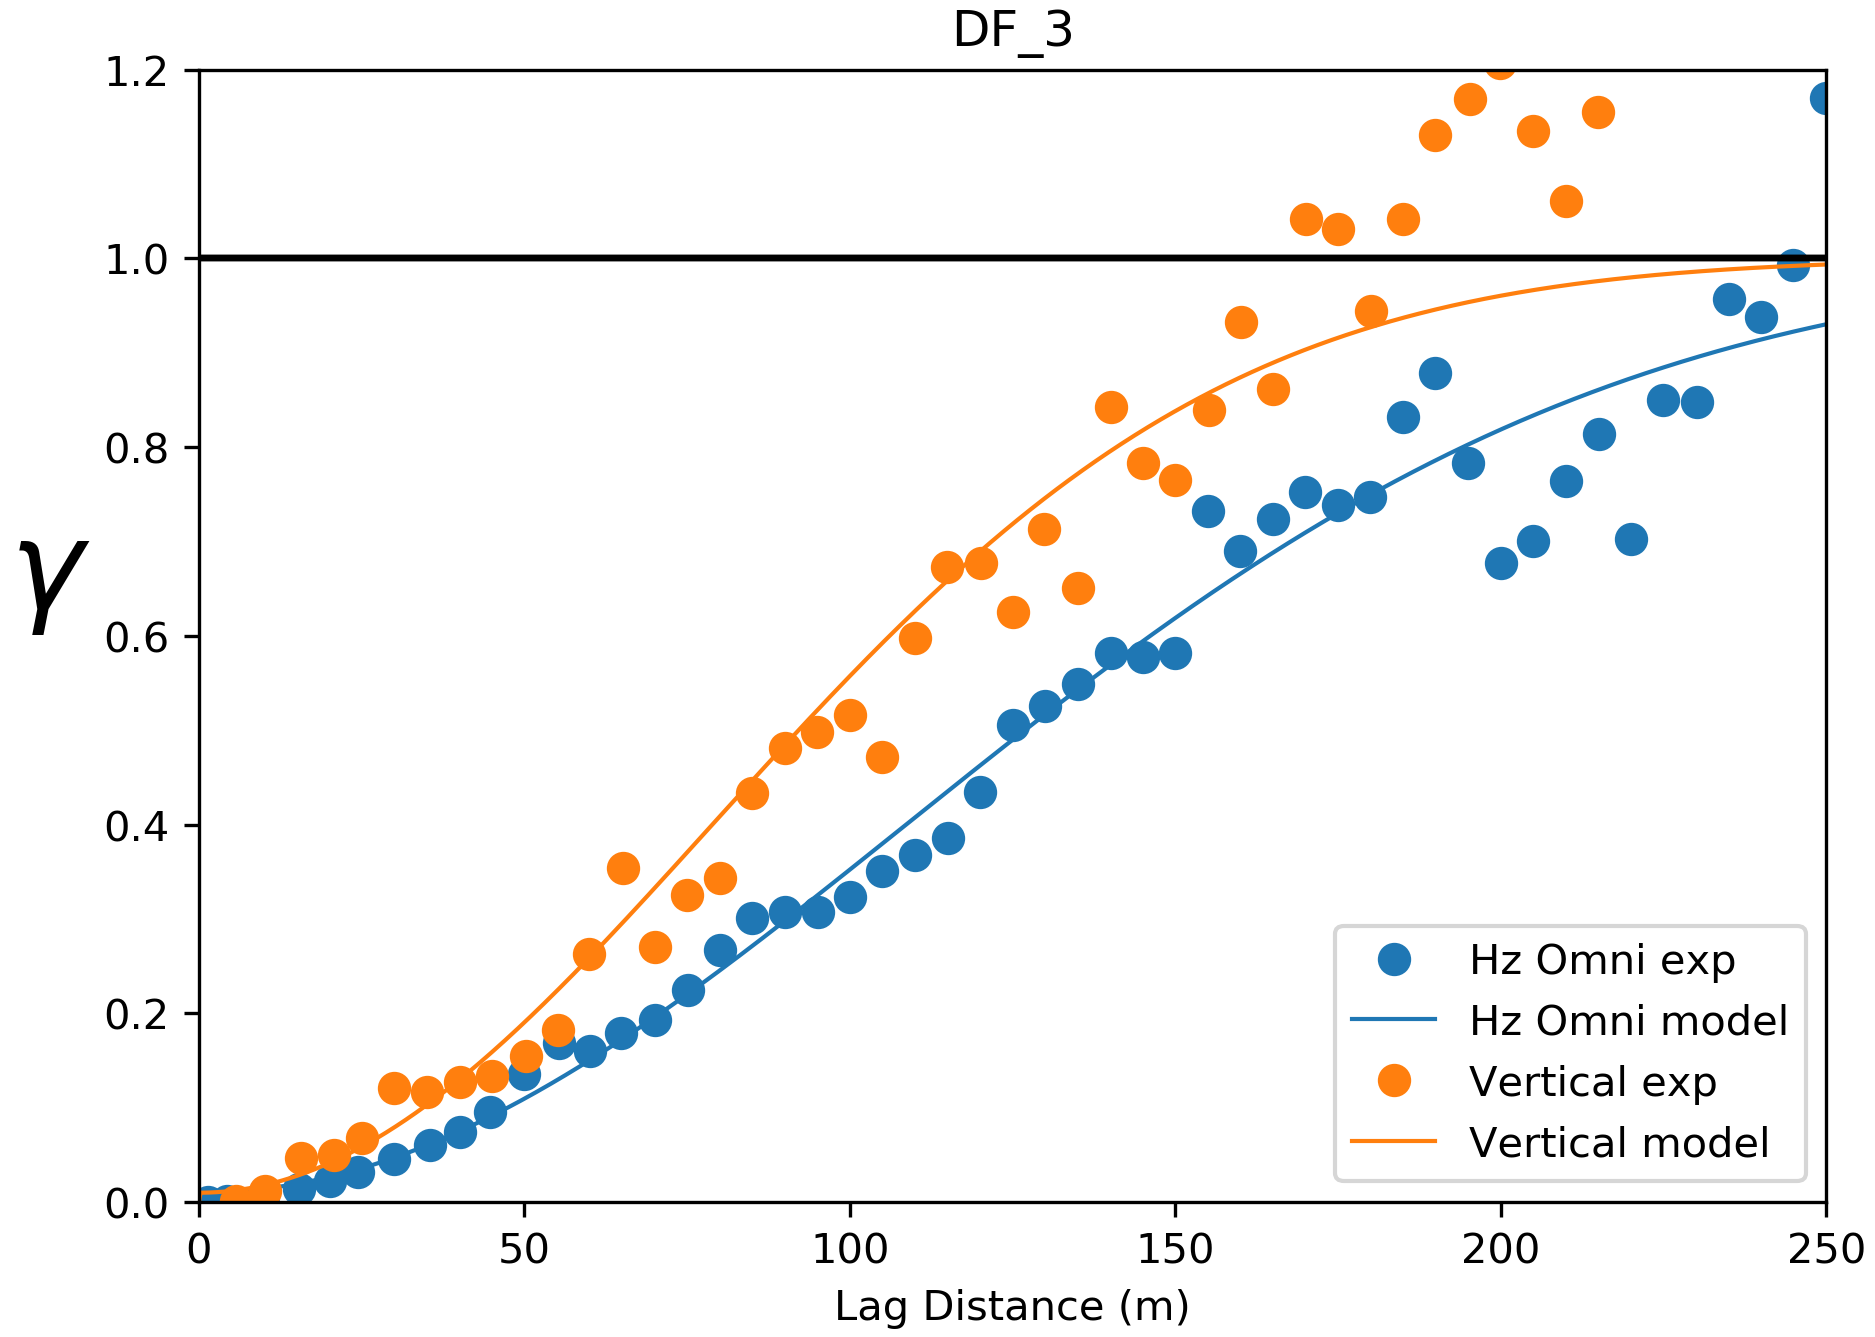
\includegraphics[width=.3\textwidth]{capitulo_2/var_DF_3.png}\label{<figure2>}}
\end{figure}
\note{Esse slide mostra os variogramas das distâncias asssinaladas calculados e modelados a partir do modelo gaussiano para as três litologias. Aqui eu calculei o variograma estandarizado, Então defino o range na variância igual a um, mas note que o valor da variância continua aumentando.
}
\end{frame}

\begin{frame}{Variogramas dos indicadores}
	\begin{figure}[H] 
		\caption{Variogramas experimentais dos indicadores e modelos para cada uma das categorias do banco de dados.} \label{ind_var}
		\centering
		\subfloat[][Categoria 1]{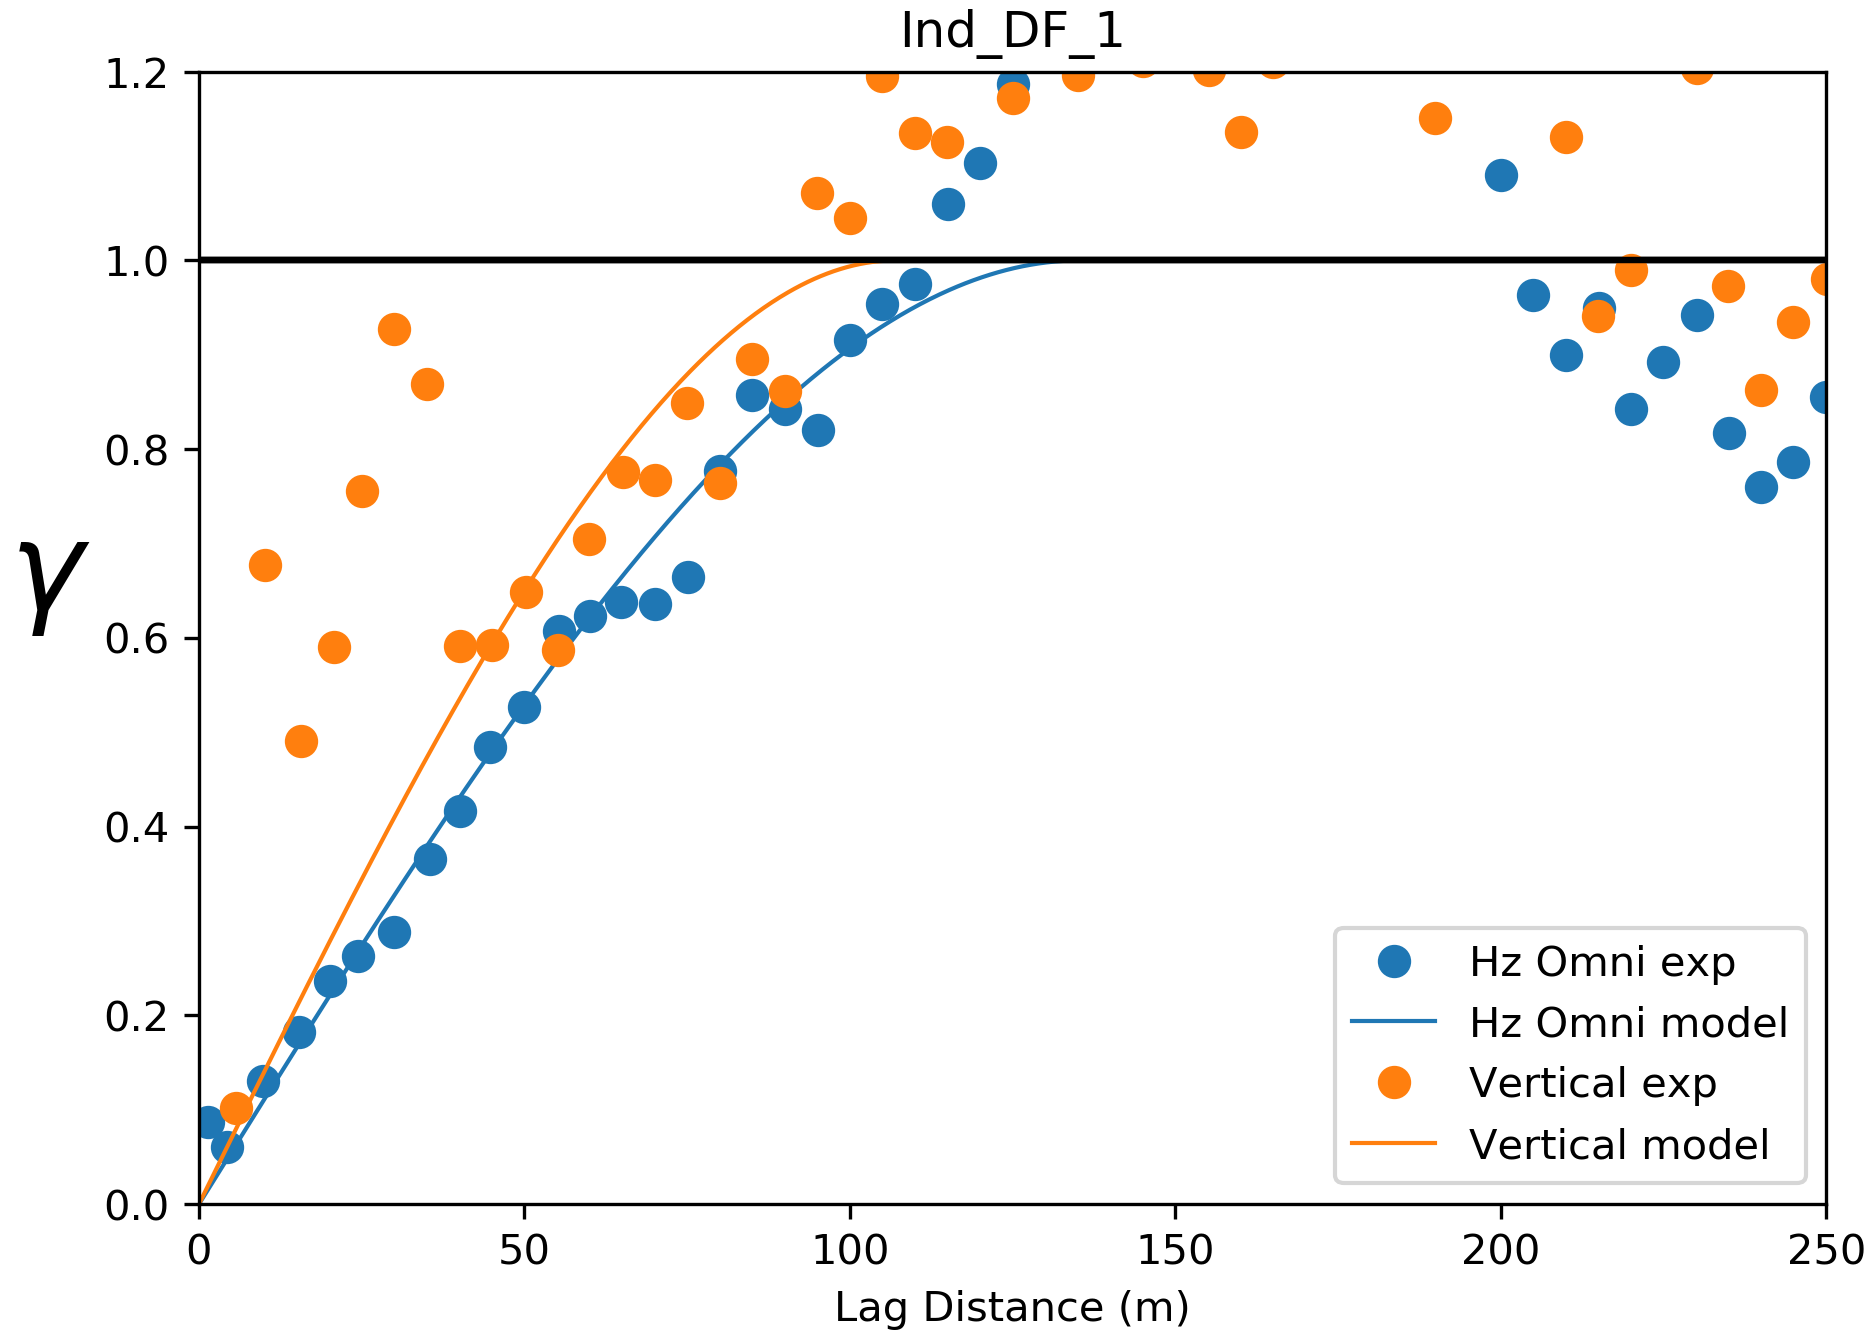
\includegraphics[width=.3\textwidth]{capitulo_2/var_Ind_DF_1.png}\label{<figure1>}}
		\subfloat[][Categoria 2]{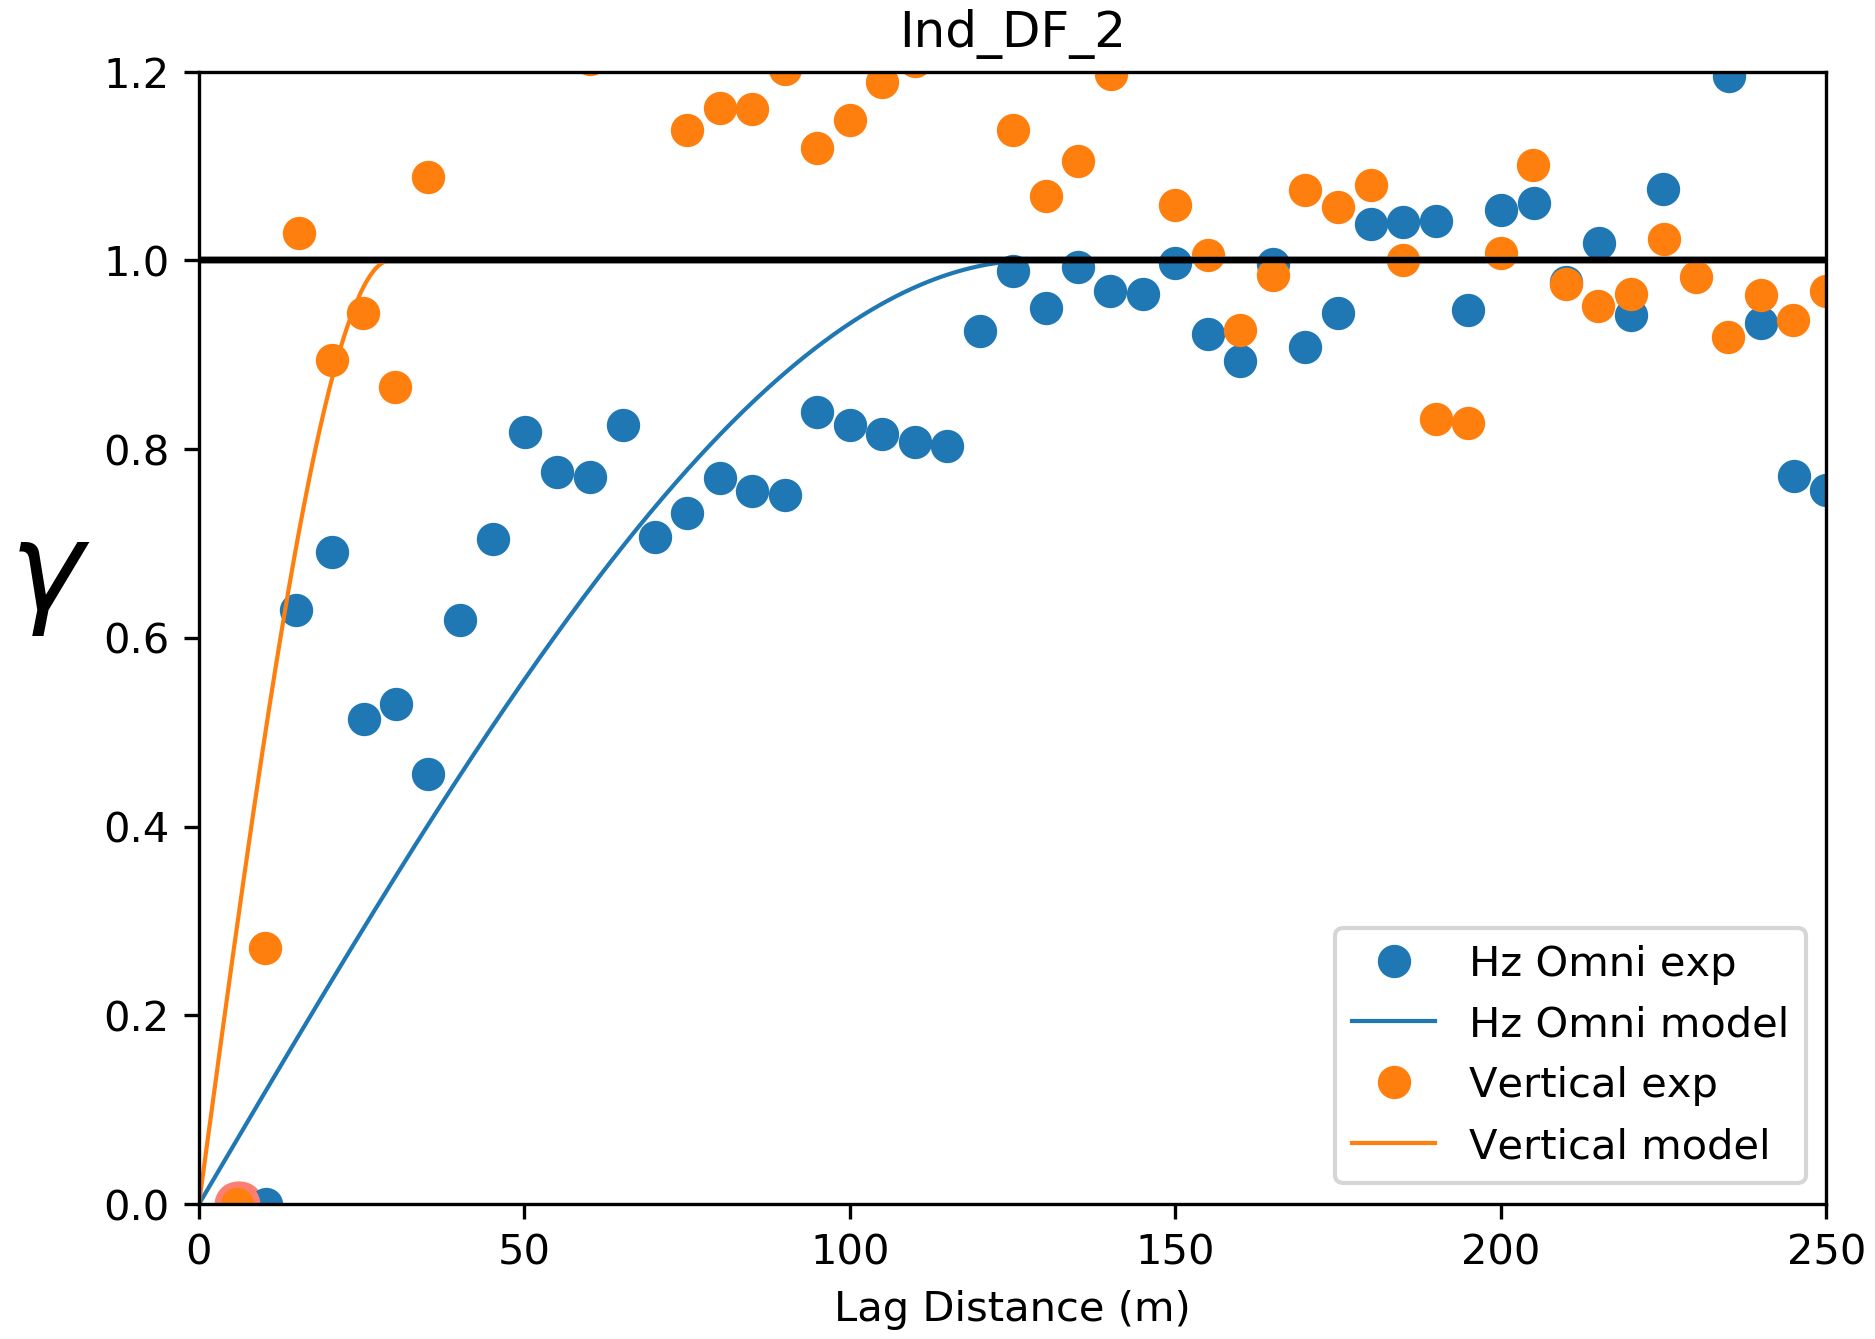
\includegraphics[width=.3\textwidth]{capitulo_2/var_Ind_DF_2.png}\label{<figure2>}}
		\subfloat[][Categoria 3]{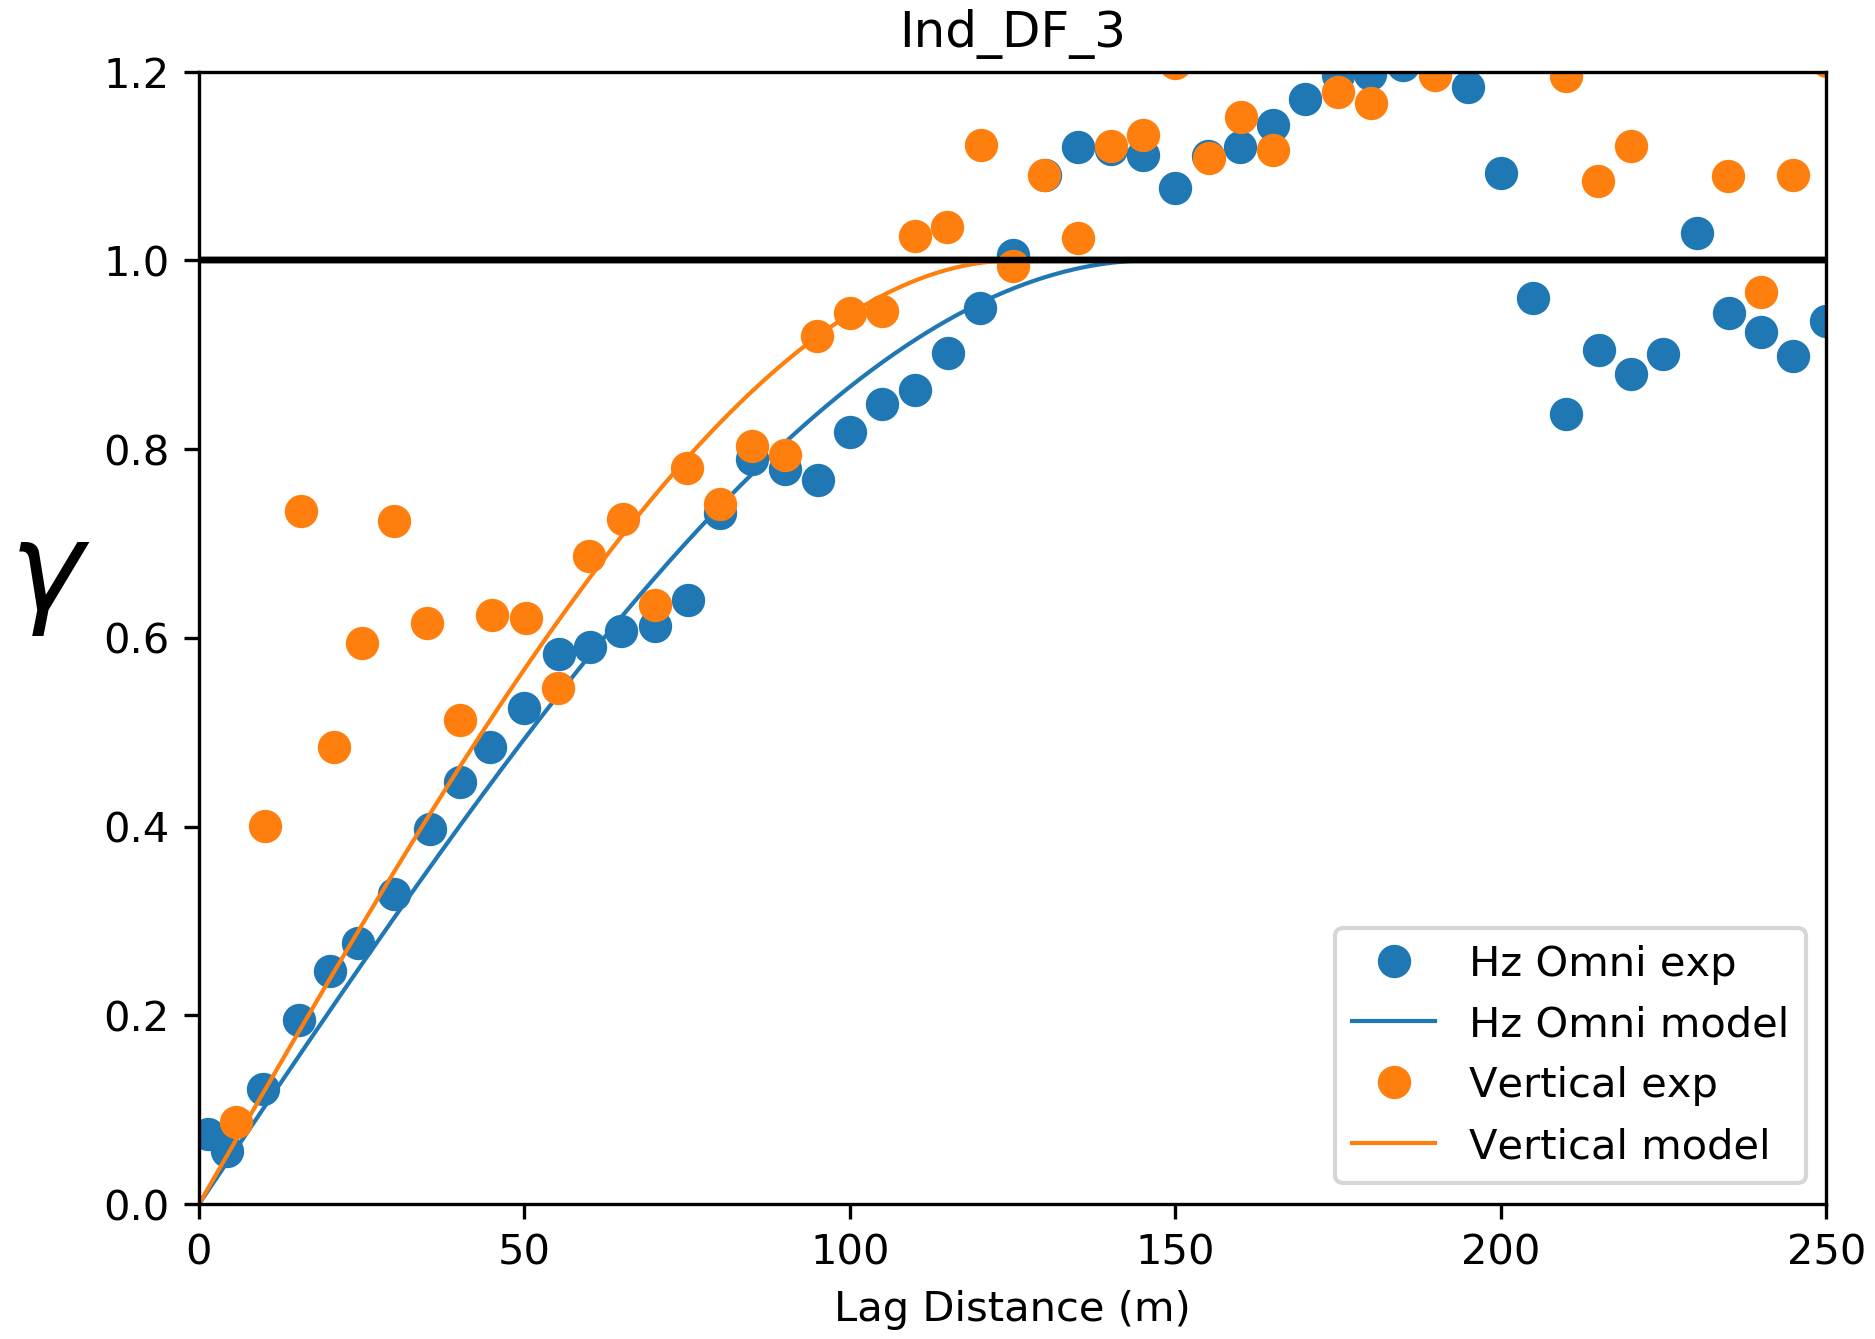
\includegraphics[width=.3\textwidth]{capitulo_2/var_Ind_DF_3.png}\label{<figure2>}}
	\end{figure}
\note{Já esse slide mostra os variograma calculados e modelados a partir do modelo esférico para os indicadores de cada categoria. Em tese, os variogramas dos indicadores são mais fáceis de modelar e são estacionários. Mas na prática, muitas vezes os variogramas dos indicadores são mais ruidosos e menos estruturados do 	que o das das distâncias assinaladas.
}
\end{frame}

\begin{frame}{Alternativa ao cálculo e modelagem dos variogramas}
	\begin{figure}[H]
		\caption{\label{cov_table}Fluxograma da modelagem geológica implícita usando tabelas de covariância.}
		\begin{center}
			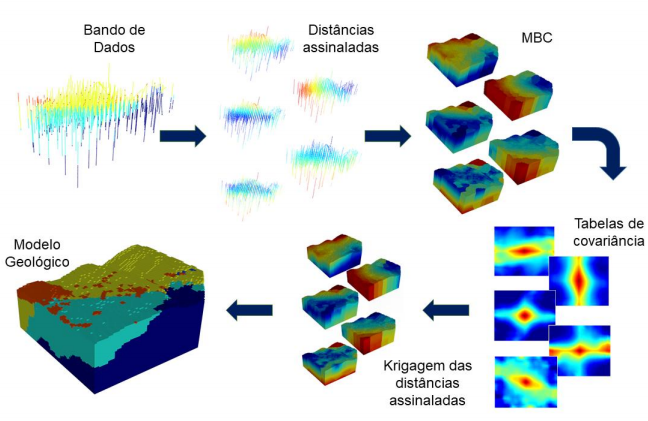
\includegraphics[width=0.7\textwidth]{capitulo_2/cov_table.png}
		\end{center}
		%\legend{\citeonline{kloechner_cov_table}}
	\end{figure}
\note{Além das alternativas sugeridas pela literatura para modelagem do variograma, aqui no laboratório a gente testou as tabelas de covariância: nesse método a partir dos dados eu crio um modelo base de covariância de onde é possível derivar, usando transformada de fourrier, a tabela de covariâcia que pode ser usada no processo de estimativa ou simulação. 
	
	Os resultados são promissores, torna o método completamente automático, sem nenhuma interferência do usuário. Porém, ainda existem alguns problemas operacionais com as tableas de covariância que não permitem uma aplicação geral pra qualquer tipo de depósito.}
\end{frame}

\subsection{Interpolação das distâncias assinaladas}

\begin{frame}{Resolução do grid}

\begin{figure}[H]
	\caption{\label{grid_res}Efeito da resolução do \textit{grid} na reprodução de estruturas geológicas.}
	\begin{center}
		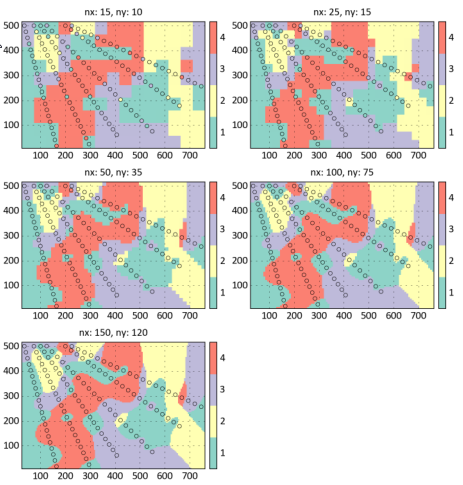
\includegraphics[width=0.4\textwidth]{capitulo_2/grid_res.png}
	\end{center}
	%\legend{Fonte: \citeonline{martin2017implicitmodeling}}
	\note{Essas ditâncias calculadas e variografadas devem ser interpoladas para todos os nós de um grid. Embora os métodos implícitos sejam gridless, que dizer, eles não dependem de um grid, os algoritmos de extração de iso superfícice exigem que a propriedade exista em um grid regular.  
		
		Para um número constante de amostras o tempo necessário para interpolar a função volume aumenta linearmente com o número de nós. Os parâmetros do grid, muitas vezes são determinados por parâmetros técnicos do projeto. Porém, para a definição do modelo geológico é impotante que o grid possa reproduzir a menor estrutura geológica de interesse.
		
		Essa imagem mostra um modelo geológico multi categórico em grids de diferentes resoluões: para as dimensões 15 por 10 parecem muito grosseiros e as categorias dos pontos amostrais não são reproduzidas, já a dimensão 25 por 15 eu ganho um pouco de resolução, mas as estruturas  ainda não tem uma forma geológica. Pra 50 por 35 as formas o modelo se suavizam, mas ainda tem algum serrilhado, 100 por 75 as formas estão bastante suaves e as categorias das amostras são reproduzidas. Pra 150 por 120 não parece haver significativa melhora em relação ao modelo anterior. 
		
		Então é preciso encontrar um balanço entre resolução e tempo de interpolação, nesse caso algo entre 50 por 35 e 100 por 75, a resolução pode aumnetar a medida que o projeto avança e mais amostras são obtidas.}
\end{figure}

\end{frame}

\begin{frame}{Grids criados}
	\begin{table}[H]
		\centering
		\begin{tabular}{lrr}
			& \multicolumn{1}{l}{Grosso} & \multicolumn{1}{l}{Fino} \\ \hline
			nx & 49 & 97 \\
			ny & 49 & 98 \\
			nz & 51 & 102 \\
			sx & 10m & 5m \\
			sy & 10m & 5m \\
			sz & 4m & 2m \\
			num & 122451 & 969612 \\ \hline
		\end{tabular}
		%\caption{Parâmetros dos \textit{grids} de definição dos modelos geológicos implícitos.} \label{grid_def}
	\end{table}
\note{Par aesse estudo de caso, dois grid foram criados, um grosso com aproximadamente 100 mil nós e um fino com aproximadamente 1 milhão de nós.
}
\end{frame}

\begin{frame}{Métodos de interpolação}
	\begin{itemize}
		\item \cite{hosseini_deutsch_iqd} utilizaram inverso da distância;
		\item \cite{silvaenhancedgeomodeling} utilizou krigagem ordinária global;
		\item \cite{rolo_dissertacao} utilizou krigagem ordinária;
		\item \cite{silva_dual} aplicaram \textit{dual kriging};
		\item \cite{boisvert_geomodeling} gerou modelos implícitos através de distâncias assinaladas com anisotropia variável local (\textit{Locally varying anisotropy kriging - LVA});
		\item \cite{manchuck_MLS} propuseram a utilização de mínimos quadrados móveis para incorporar interpretação manual e avaliar incerteza.
	\end{itemize}
\note{Qualquer método de interpolação pode ser usado para as distâncias assinaladas, até mesmo métodos do inverso da distância produzem resultados realistas. A krigagem e as funções de bases radiais permitem incorporar informaçõ adicional através dos modelos de covariância, porém a literatura recomenda o uso de métodos globais, ouseja, que usa, todas as amostras em todas as estimativas.
	
	Diferentes métodos de interpolação podem ser encontrados na literatura:
	
	* housseini e deutcsh usaram iqd;
	
	* SIlva usou krigagem ordinária global;
	
	* Eu usei krigagem ordinária na minha dissertação;
	
	* O Boisvert usa LVA kriging pra interpolar com anistropia local;
	
	* e o jonh manchuck e o clayton propusera um novo método de interpolação que integra seções digitalizadas e amostras.}
\end{frame}

\begin{frame}{Métodos de interpolação}
	\begin{figure}[H] 
		\caption{Interpolação das distâncias calculadas por diferentes métodos.} \label{interpo}
		\centering
		\subfloat[][OK com 40 amostras]{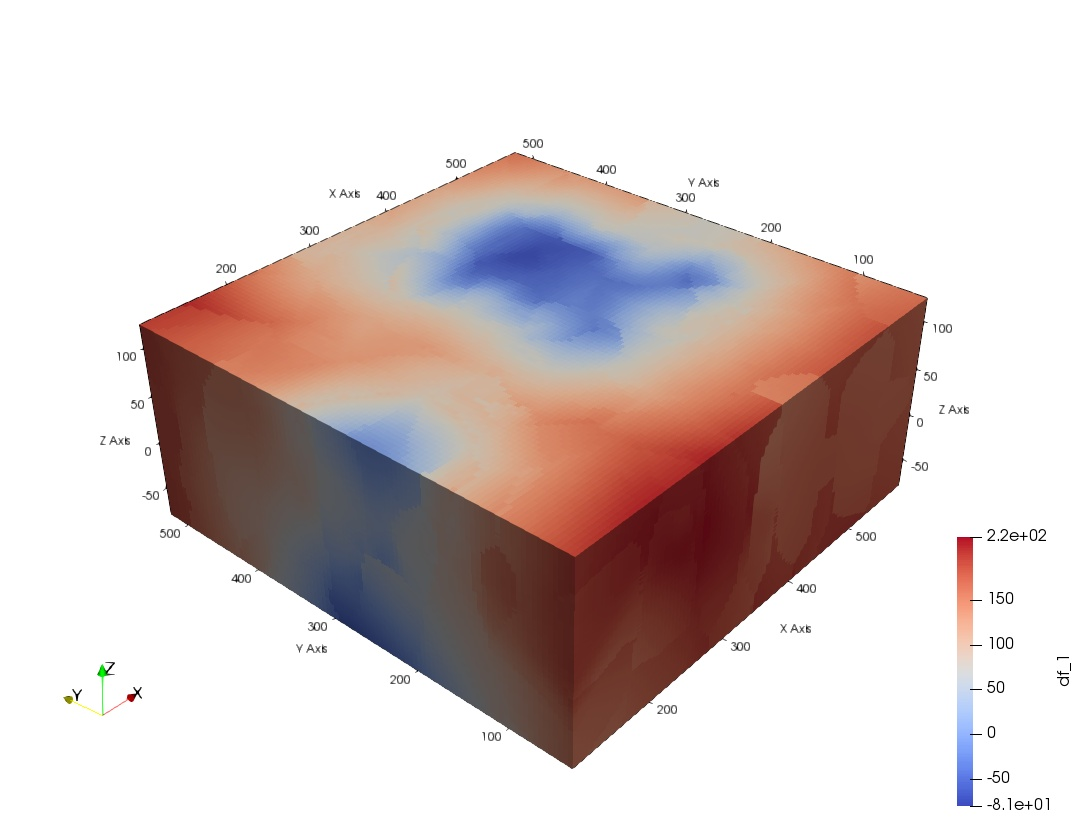
\includegraphics[width=.3\textwidth]{capitulo_2/kt3d40.jpeg}\label{<figure1>}}
		\subfloat[][OK com 100 amostras]{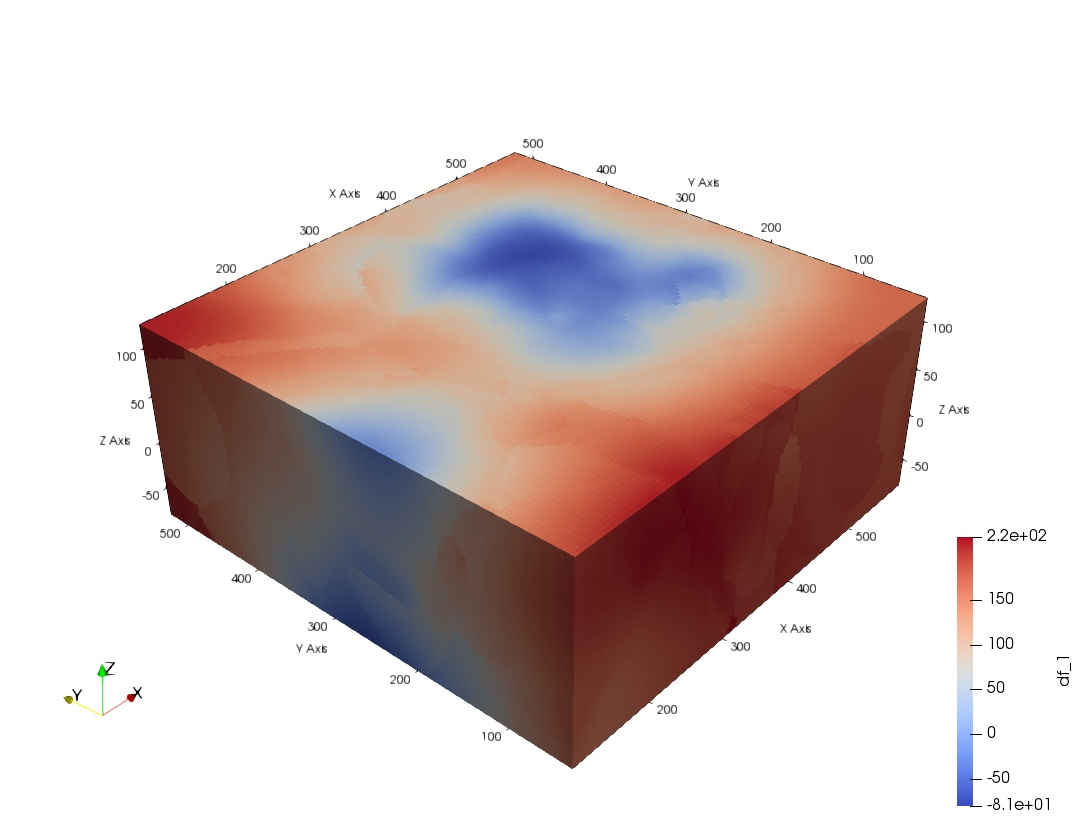
\includegraphics[width=.3\textwidth]{capitulo_2/kt3d100.jpeg}\label{<figure2>}}
		\subfloat[][RBF global]{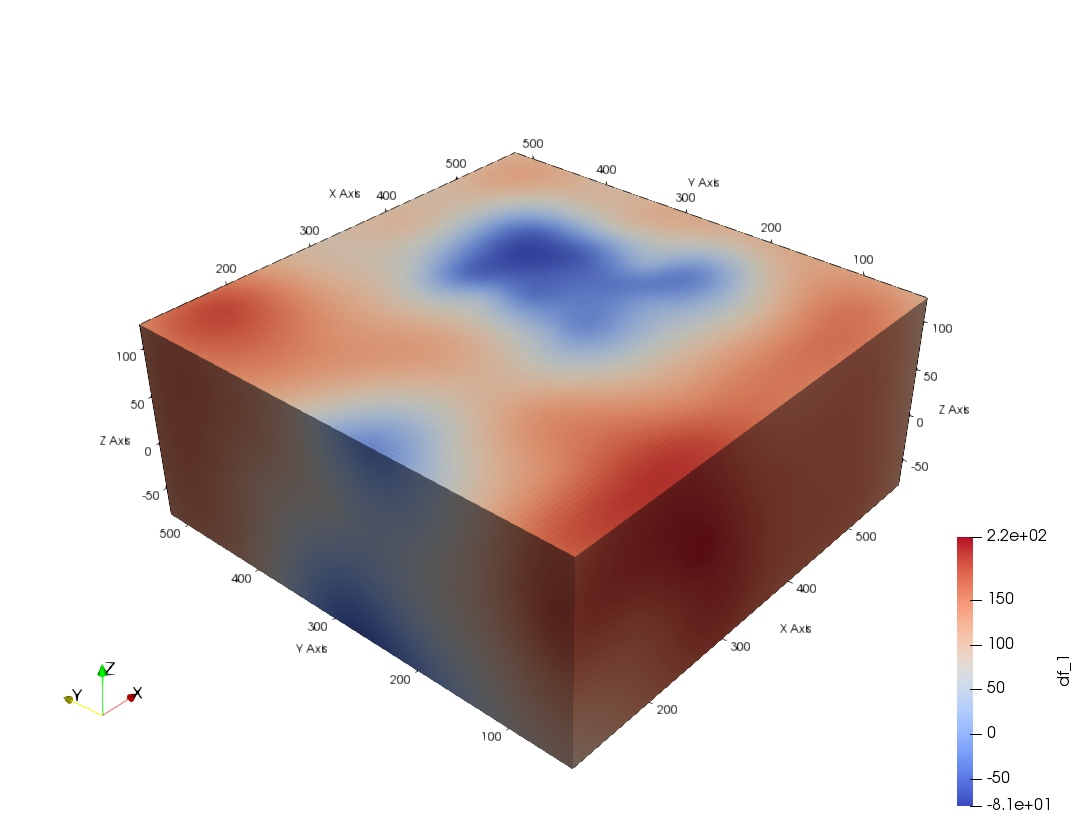
\includegraphics[width=.3\textwidth]{capitulo_2/rbf.jpeg}\label{<figure2>}}
	\end{figure}
\note{Esse slide mostra o porquê  de usar métodos globais. O primeiro modelo foi interpolado por krigagem ordinária usando 40 amostras por estimaitva, e fica bem evidente o surgimento de artefatos, causados pela estratégia de busca. O segundo modelo foi interpolado com 100 amostras por estimativa e mesmo assim ainda é possível observar artefatos no modelo. O último modelo foi interpolado por RBF, que é um método global e gera modelos suaves e livres de artefatos.}
\end{frame}

\begin{frame}{Decomposição do domínio}

Transforma um problema volumoso e que demanda muito esforço computacional em diversos problemas menores e eficientes que são, ao final, unidos.

\begin{figure}[H]
	\caption{\label{pou}Esquema mostrando o particionamento.}
	\begin{center}
		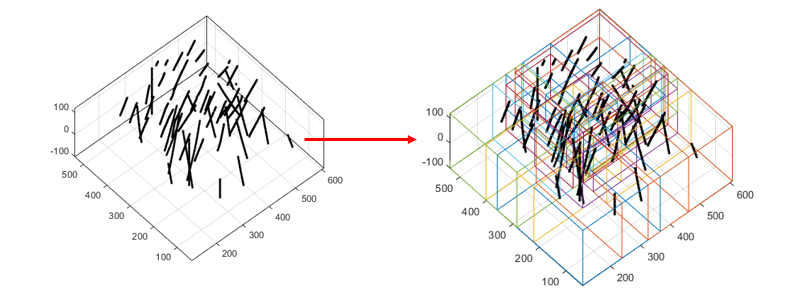
\includegraphics[width=0.9\textwidth]{capitulo_2/pou.jpg}
	\end{center}
	%\legend{Fonte: \citeonline{martin_boisvert_review_rbf}}
\end{figure}
\note{Apesar de que nos métodos globais a matriz de covariâcias das amostras com elas mesmo só precise ser invertida uma vez, para bancos de dados volumosos isso ainda é uma tarefa que demanda um grande esformço computacional, então, é possível particionar o problema em problemas menores, sobrepostos, que são mais eficientes, e unir todas as partes.}
\end{frame}

\begin{frame}{Benchmark}

Todos os algoritmos utilizados são da biblioteca GSLib e foram executados em um core i7 7700HQ @ 2.8 GHz com 16 Gb de RAM.

\begin{table}[H]
	\centering
	\resizebox{\textwidth}{!}{%
		\begin{tabular}{lllll}
			Método & Tempo grid grosso & Tempo grid fino & Classificação errônea grosso & Classificação errônea fino \\ \hline
			krigagem global isotrópica & 28min &  & 121 &  \\
			krigagem global anisotrópica & 30min 34s &  & 282 &  \\
			krigagem ordinária anisotrópica (40) & 1min 3s & 38min & 137 & 135 \\
			krigagem ordinária anisotrópica (100) &  & 45min 51s &  & 181 \\
			RBF isotrópico & 21.5s &  & 57 &  \\
			RBF anisotrópico &  & 1min 22s &  & 38 \\
			Particionado RBF anisotrópico &  & 1min 2s &  & 39 \\
			Particionado RBF artefatos & 16.5s &  &  & 29 \\
			LVA OK &  &  & 8 &  \\
			LVA RBF &  &  &  & 8 \\
			Krigagem dos indicadores &  & 33min 27s &  & 2 \\ \hline
		\end{tabular}%
	}
	%\caption{\textit{Benchmark} dos diferentes métodos de interpolação.} \label{bench}
\end{table}
\note{Essa tabela mostra um benchmark dos métodos de interpolação para o banco de dados apresentado, as distâncias foram interpoladas por diferentes métodos no grid grosso que tem 100 mil nós e no grid fino com 1 milhão.
	
	Todos os algoritmos são da biblioteca GSLib e foram rodados em um notebook comercial high end, para as três categorias.
	
	Eu queria destacar algus pontos: não é possível interpolar as distância no grid fino por krigagem global, mesmo com 16gb de ram. A krigagem ordinária no grid fino, isso para as três categorias, leva 45 minutos, enquanto o RBF leva apenas pouco mais de um minuto, ainda é possível reduzir esse tempo particionando o grid.
	
	Não é difícil perceber porque o RBF é o método preferido para interpolação de distâncias assinaladas, além de produzir modelos suaves, desejáveis nesse contexto de modelagem geológica, é 10 vezes mais rápido que a krigagem.
	
	A Leapgfrog tem um algoritmo de rbf patenteado, chamado fast rbf, que é ainda mais rápido.}
\end{frame}

\subsection{Visualização do modelo geológico}

\begin{frame}{Visualização do modelo geológico}

Um bom palpite inicial para a interface que separa os domínios no espaço, seria a linha (em duas dimensões) ou superfície (em três dimensões) que corresponda ao valor zero da função distância assinalada

\begin{figure}[H]
	\caption{Iso superfícies para a categoria 1 extraída dos diferentes modelos implícitos.} \label{isosup}
	\centering
	\subfloat[][OK com 40 amostras]{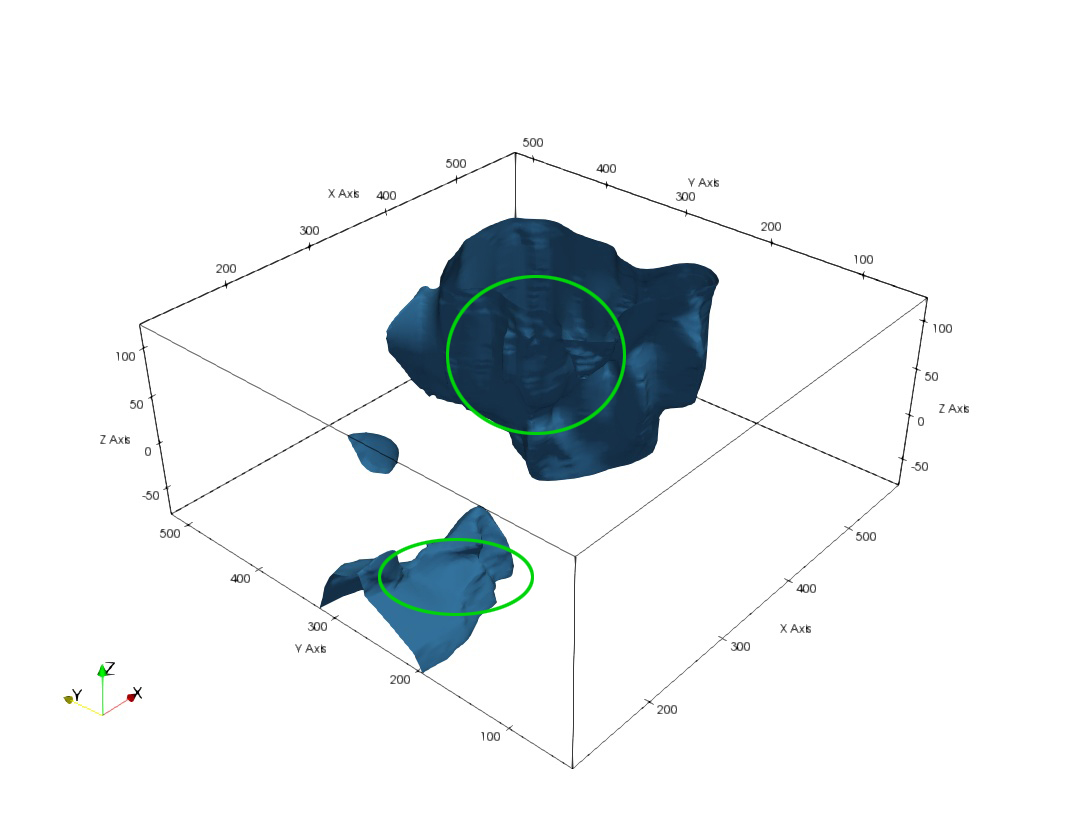
\includegraphics[width=.3\textwidth]{capitulo_2/isokt3d40.jpeg}\label{<figure1>}}
	\subfloat[][OK com 100 amostras]{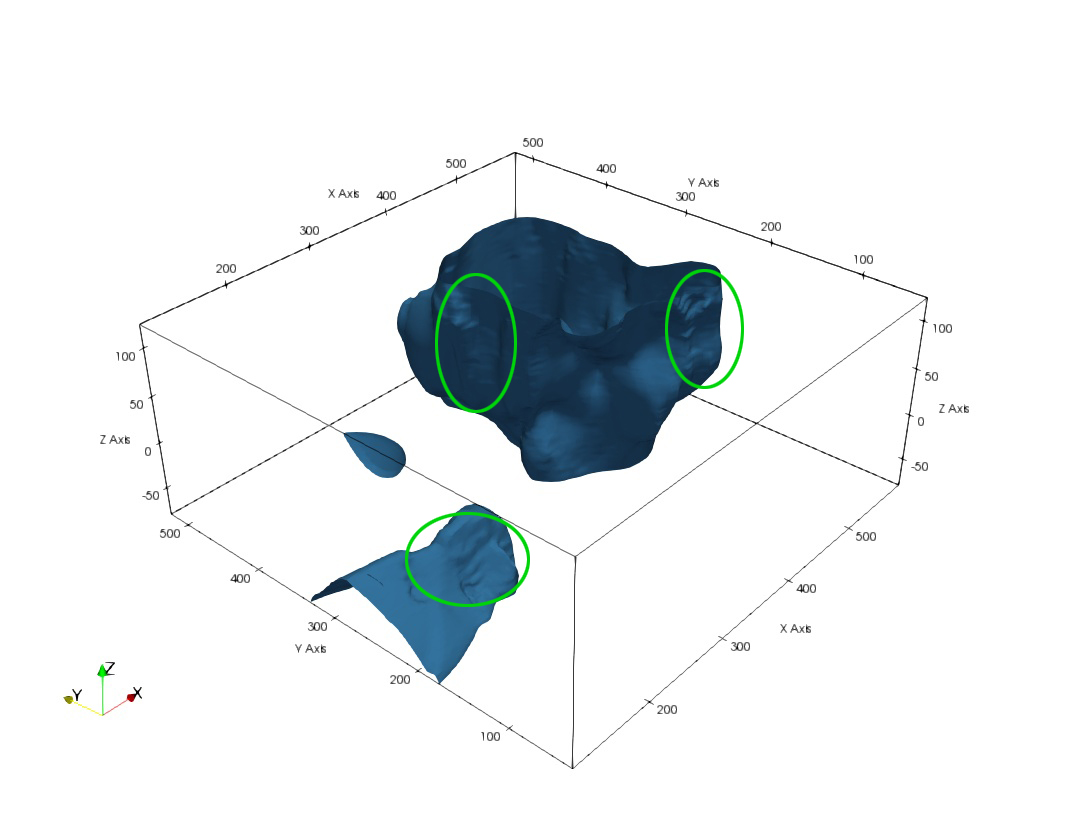
\includegraphics[width=.3\textwidth]{capitulo_2/isokt3dn100.jpeg}\label{<figure2>}}
	\subfloat[][RBF global]{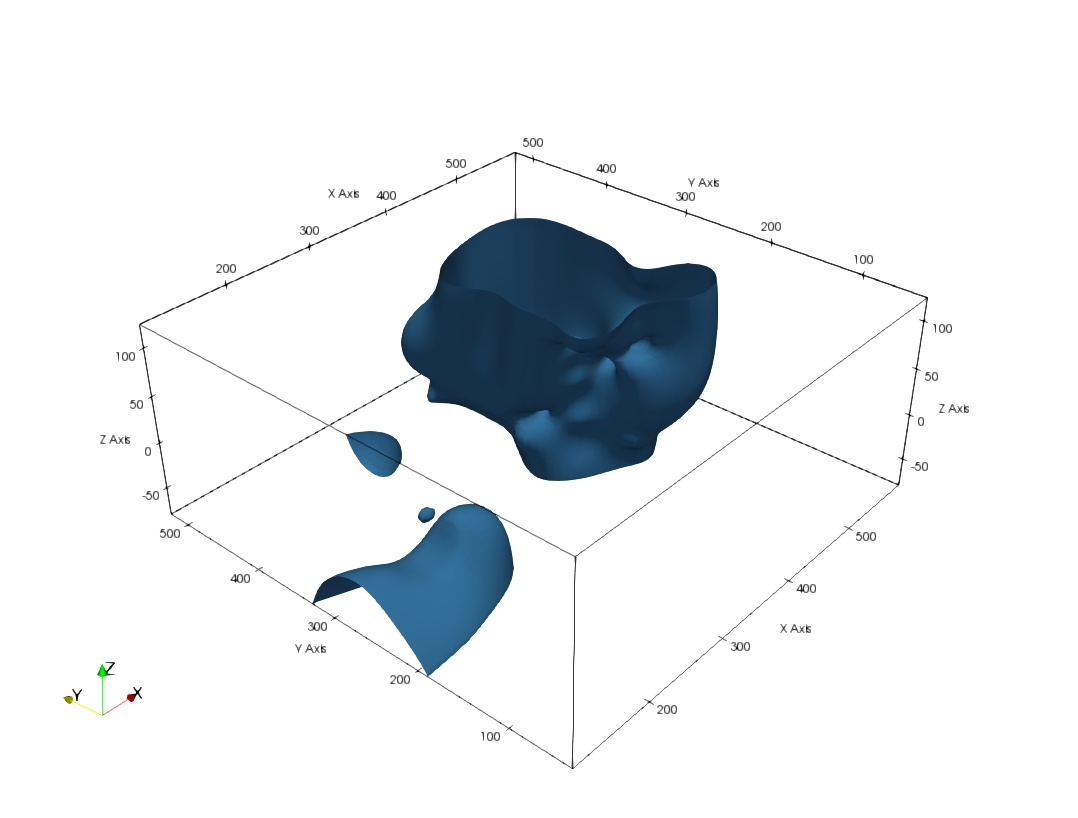
\includegraphics[width=.3\textwidth]{capitulo_2/isorbf.jpeg}\label{<figure2>}}
\end{figure}
\note{O modelo implícito, que é a função distância interpolada, tem infinitas iso usperfícies, pra visualizar o modelo geológico eu preciso extrair uma dessas superfície, e o melhor palpite pra onde se localiza a interface é a iso superfície zero. esse slide mostra a isosuperfície zero extraída, usando o algoritmo de cubos marchantes no software paraview, para a categoria 1. A partir dos modelos implícitos apresentados anteriormente. krigagem ordinária com 40 amostras, 100 amostras e rbf.
	
	É possível observar que os artefatos dos modelos implícitos são transferidos para as isosuperfícies, e que métodos globais que geram modelos suaves, naturalemtne geram iso superfícies suaves, que apresentam realismo geológico.}
\end{frame}

\begin{frame}{Visualização do modelo geológico}
	\begin{figure}[H]
		\caption{Iso superfície extraída do modelo implícito interpolado por RBF para a categoria 1.} \label{iso_cat1}
		\centering
		\subfloat[][Vista 1]{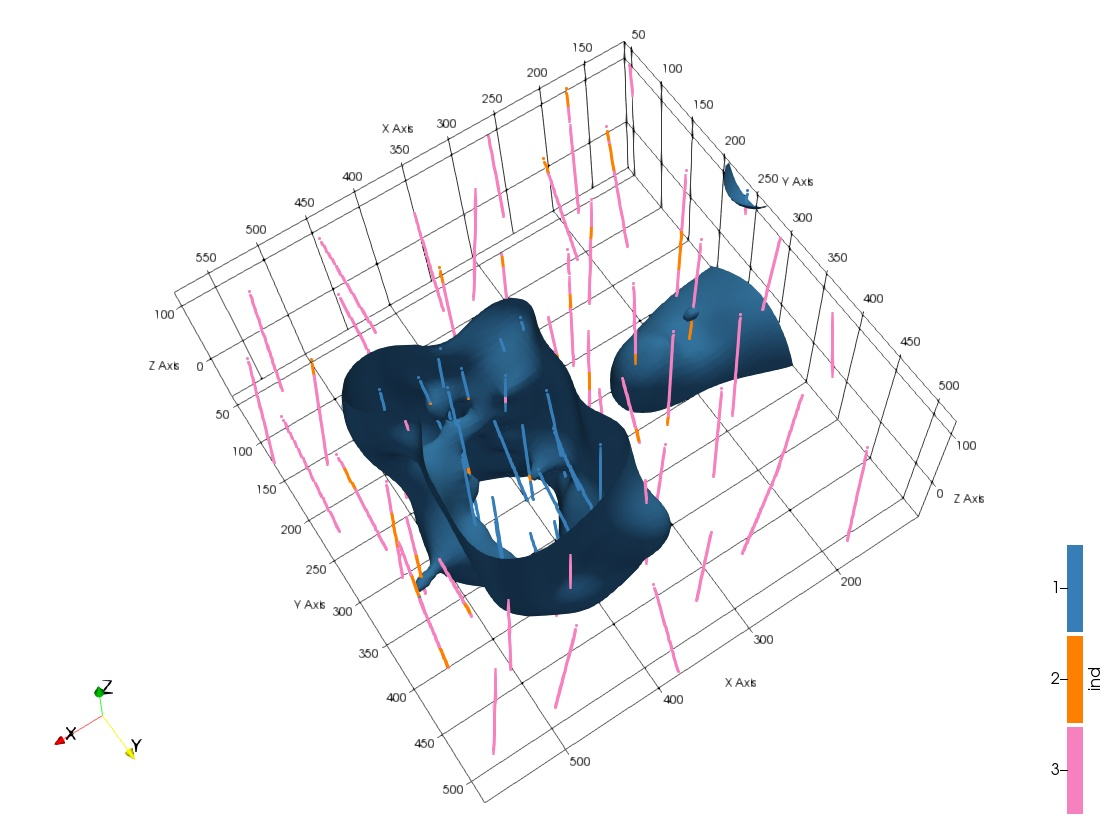
\includegraphics[width=.5\textwidth]{capitulo_2/iso_cat1_rbf.jpeg}\label{<figure1>}}
		\subfloat[][Vista 2]{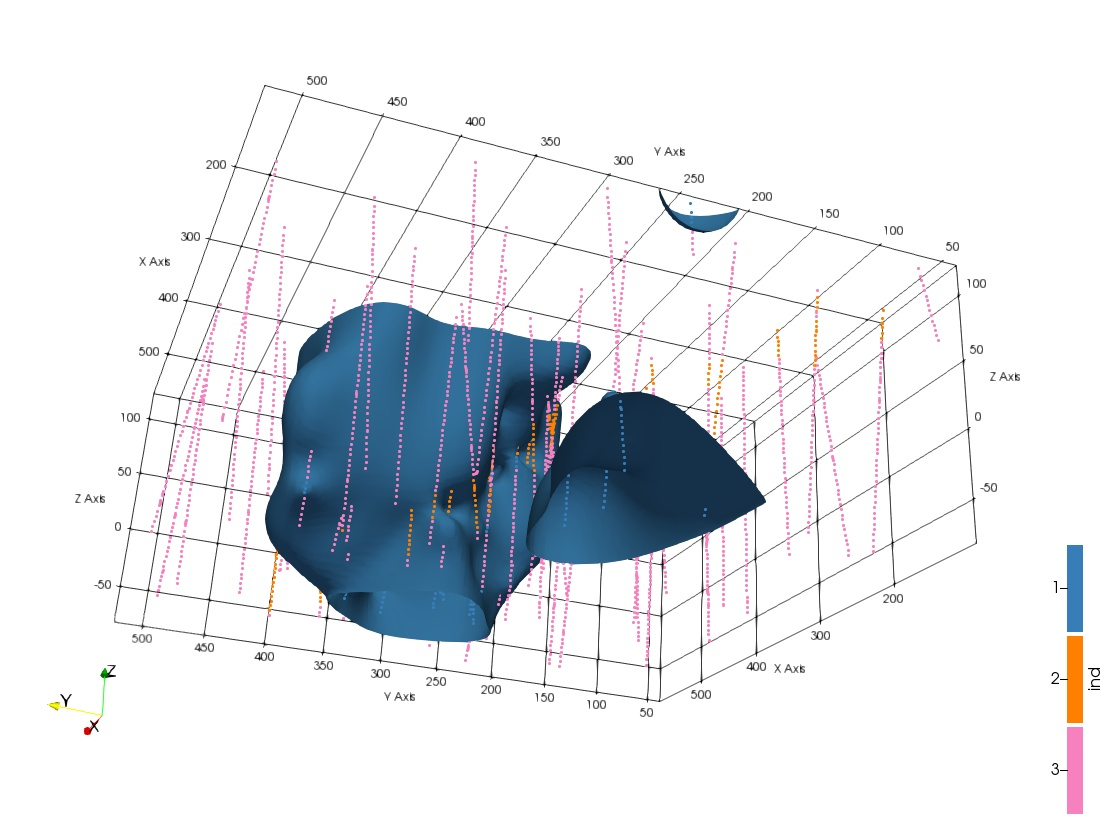
\includegraphics[width=.5\textwidth]{capitulo_2/iso_cat1_rbf2.jpeg}\label{<figure2>}}
	\end{figure}
\note{Esse slide mostra duas vistas diferentes da iso superficie zera extraida do modelo implicita interpolado por rbf para a categoria 1, junto com as amostras. Além de criar modelos realistas o rbf honra as amotras.}
\end{frame}

\begin{frame}{Visualização do modelo geológico}
\begin{figure}[H] 
	\caption{Iso superfície extraída do modelo implícito interpolado por RBF para a categoria 2.} \label{iso_cat2}
	\centering
	\subfloat[][Vista 1]{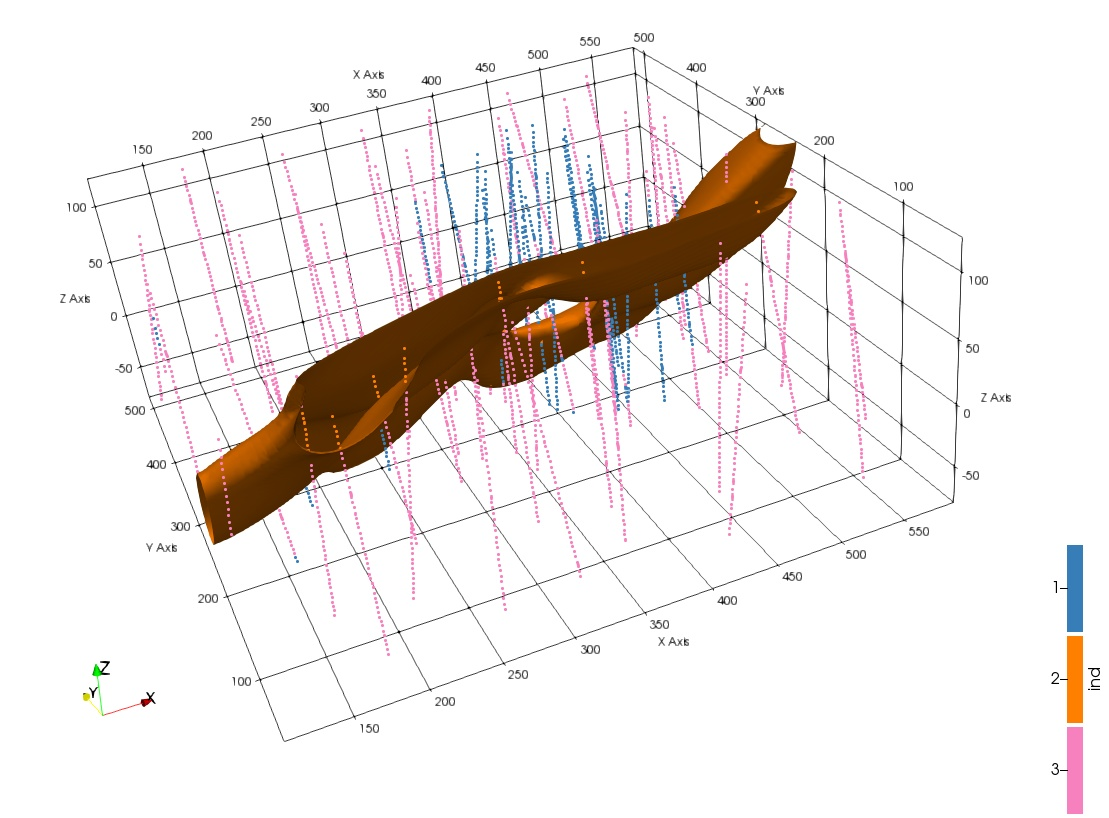
\includegraphics[width=.5\textwidth]{capitulo_2/iso_cat2_rbf.jpeg}\label{<figure1>}}
	\subfloat[][Vista 2]{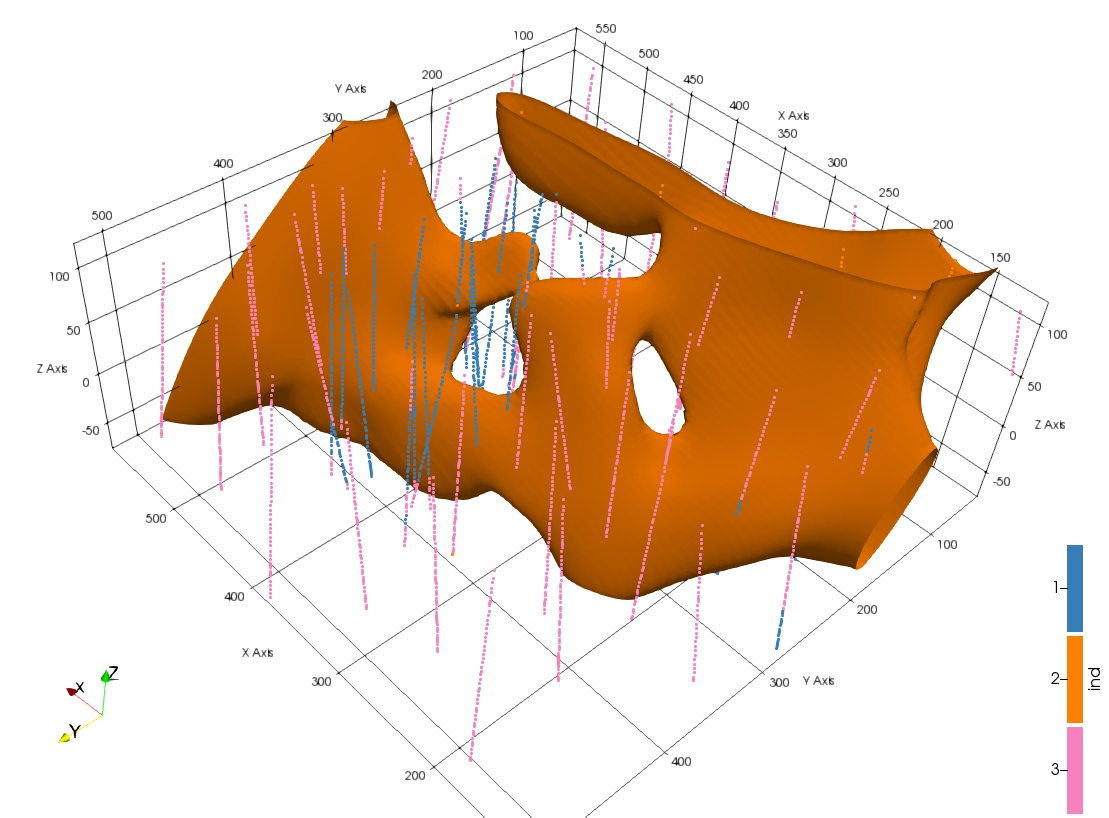
\includegraphics[width=.5\textwidth]{capitulo_2/iso_cat2_rbr2.jpeg}\label{<figure2>}}
\end{figure}
\note{E o mesmo para a categoria 2.
}
\end{frame}

\subsection{Adaptação para múltiplas categorias simultaneamente}

\begin{frame}{Adaptação para múltiplas categorias simultaneamente}

\begin{equation}
i_k(u_\alpha)=\begin{cases}
1,\:\textrm{se}\:z(u_\alpha)=k\\
0,\:\textrm{se}\:z(u_\alpha)\:\textrm{caso contrário}\end{cases} k=1,...,K
\label{eq_mult_ind}
\end{equation}

\begin{equation}
d_k(u_\alpha)=\begin{cases}
-\parallel u_\alpha-u_\beta\parallel,\:\textrm{se}\:i_k(u_\alpha)=1\\
+\parallel u_\alpha-u_\beta\parallel,\:\textrm{se}\:i_k(u_\alpha)=0\end{cases} k=1,...,K
\label{eq_mult_sg}
\end{equation}

\begin{equation}
d_k^*(u)=\sum\limits_{\alpha=1}^n \lambda_\alpha(u)d_k(u_\alpha)\quad k=1,...,K
\label{eq_mult_ok}
\end{equation}

\begin{equation}
i^*(u)=k'\;\text{de modo que}\;d_{k'}^*=min\{d_k^*(u)\}_{k=1}^K
\label{eq_mult_rt}
\end{equation}

\note{Silva e Deutsch propuseram uma adaptação para o método para modelar múltiplas categorias simultânemanete. Se existirem K multiplos dominios no depósito mineral as amostras devem ser codificadas em indicadores K vezes, as distâncias assinaladas devem ser calculadas para as K categorias, As K propriedades distâncias asssinaladas devem ser interpoladas para um mesmo grid, e a categoria responsável pela menor distância assinalada, a mais negativa, deve ser retida no local não amostrado.}

\end{frame}

\begin{frame}{Adaptação para múltiplas categorias simultaneamente}
\begin{figure}[H]
	\caption{\label{mult_cat}Esquema para criação de um modelo implícito multi categórico.}
	\begin{center}
		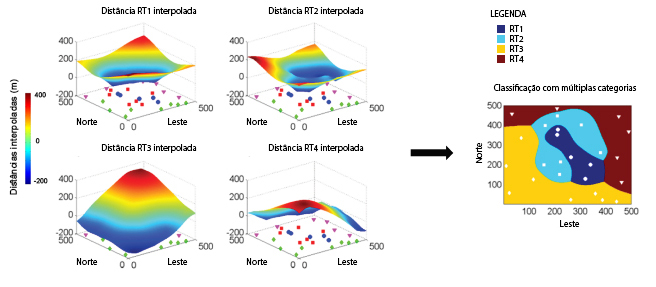
\includegraphics[width=\textwidth]{capitulo_2/mult_cat_legenda.jpg}
	\end{center}
	%\legend{Fonte: Modificado de \citeonline{silvageostatlessons}}
\end{figure}
\note{Esse slide mostra um esquema da modelagem geológica implícita para múltiplos domínios simultâneos: nas bases dos gráficos estão as amostras, no nivel superior a projeção das distâncias assinaladas interpoladas, para categoria 1 as distancias são negativas onde tem amostra da categoria 1, que é na parte central da área. mesma coisa para as categorias 2, 3 e 4. Pra cirar o modelo geológico é só reter a categoria responsável pela menor distância. na região central é a categoria 1, na parte noroeste a 3 nordeste a 4 e em volta do centro a categoria 2.}
\end{frame}

\begin{frame}{Adaptação para múltiplas categorias simultaneamente}
\begin{figure}[H]
	\caption{Modelo geológico multi categórico.} 
	\label{multi_cat_rbf}
	\centering
\subfloat[][Seções em XZ do modelo implícito gerado por RBF no \textit{grid} fino.]{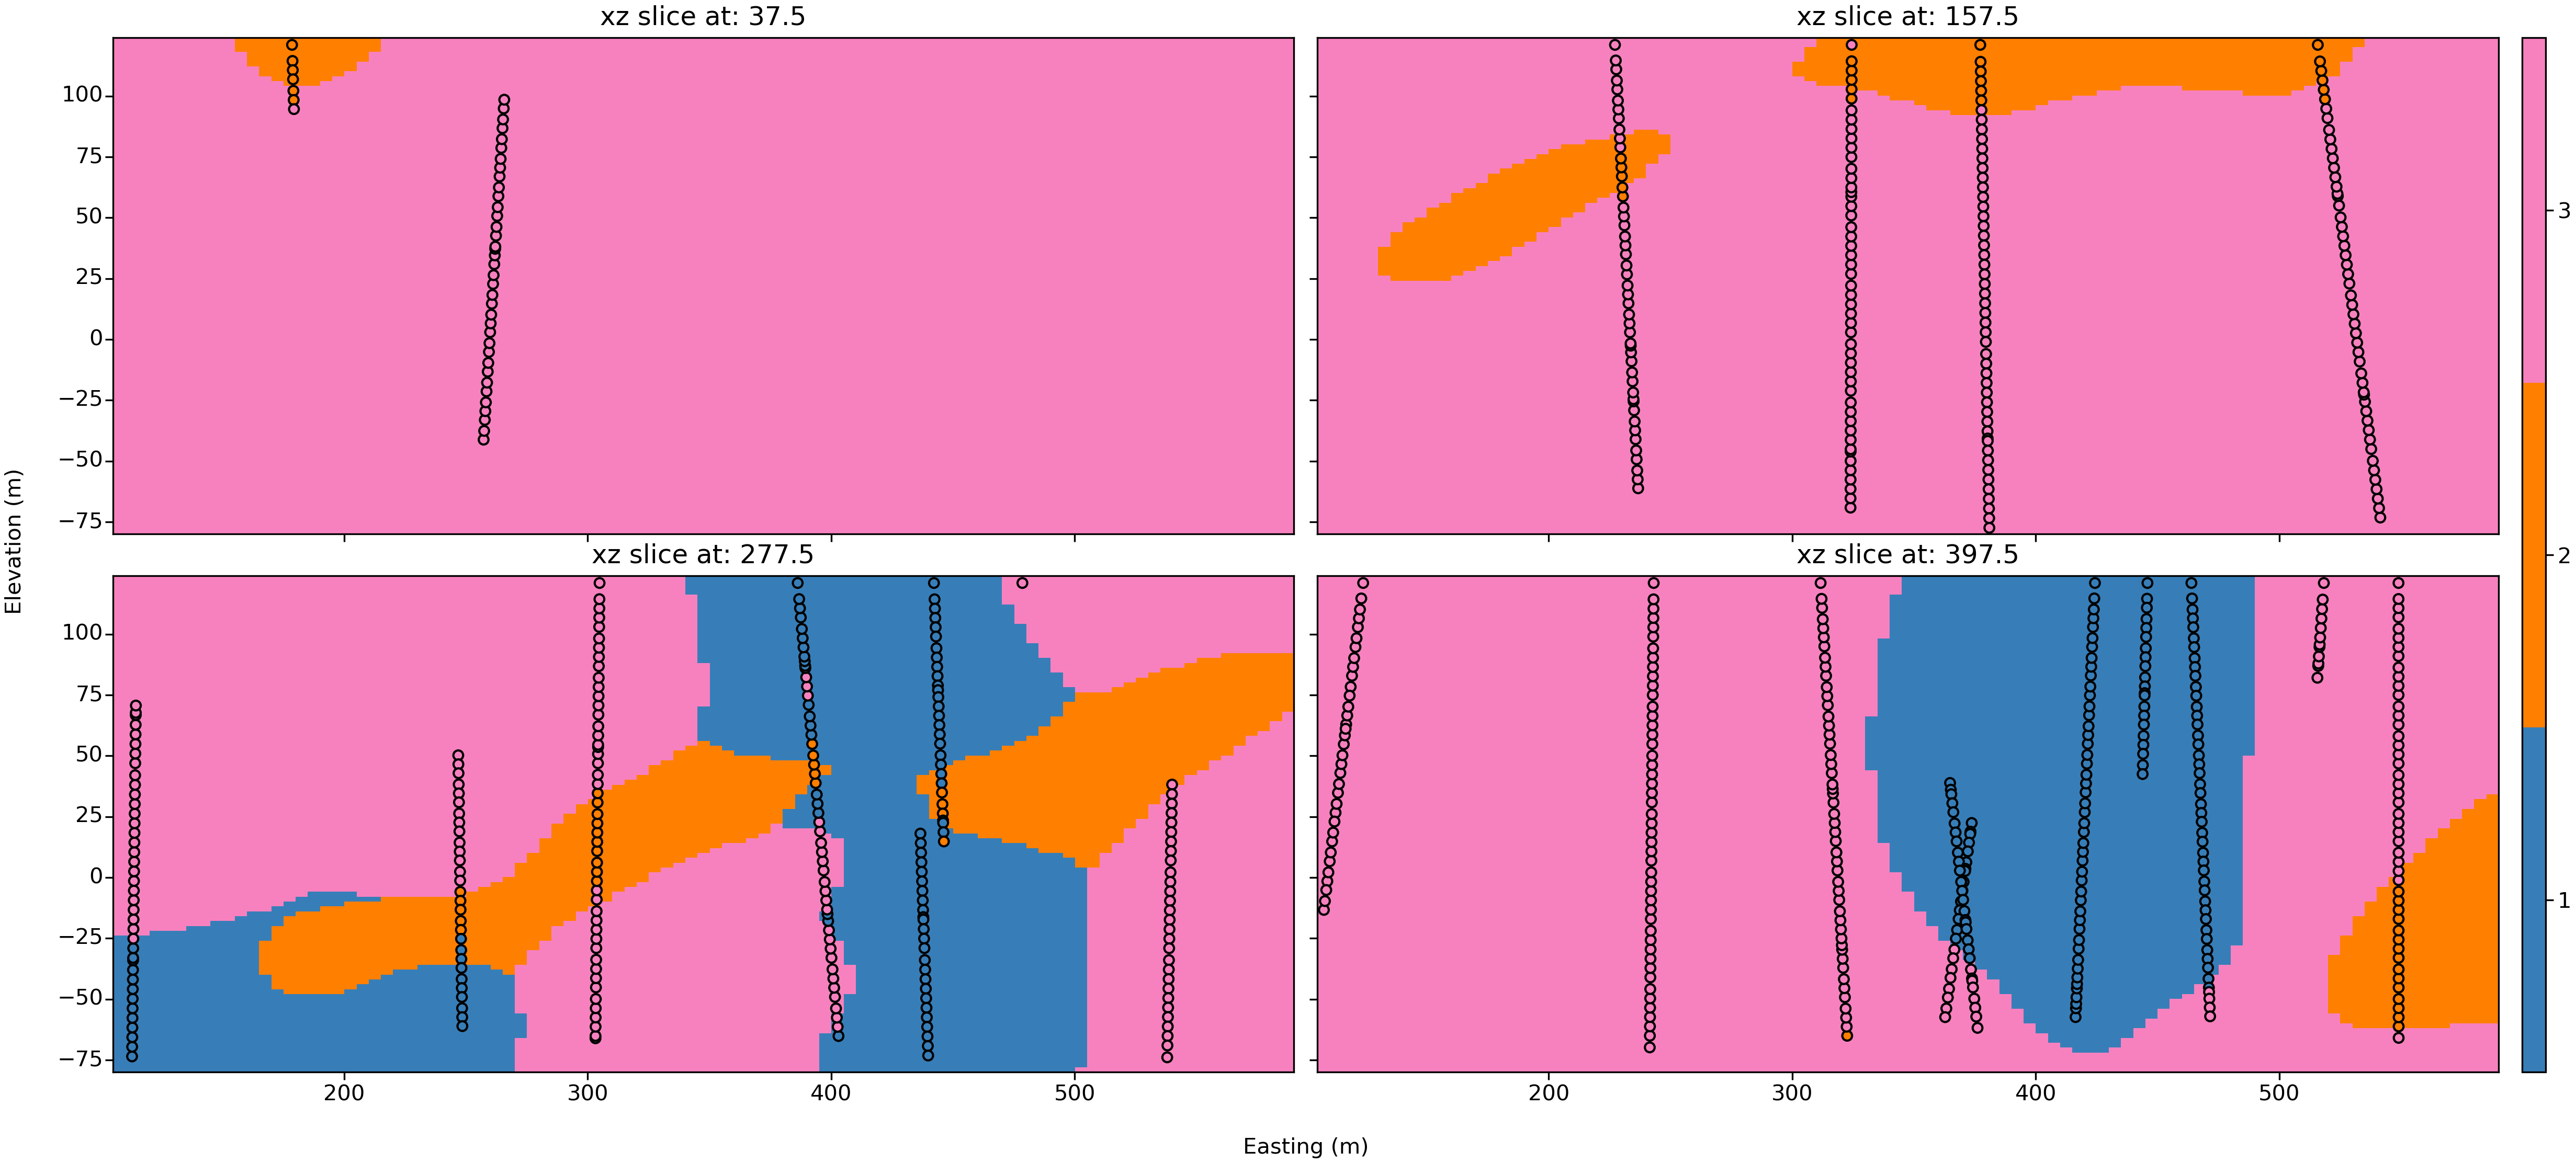
\includegraphics[width=.5\textwidth]{capitulo_2/anisofinexz.png}\label{<figure1>}}
\subfloat[][Seções em YZ do modelo implícito gerado por RBF no \textit{grid} fino.]{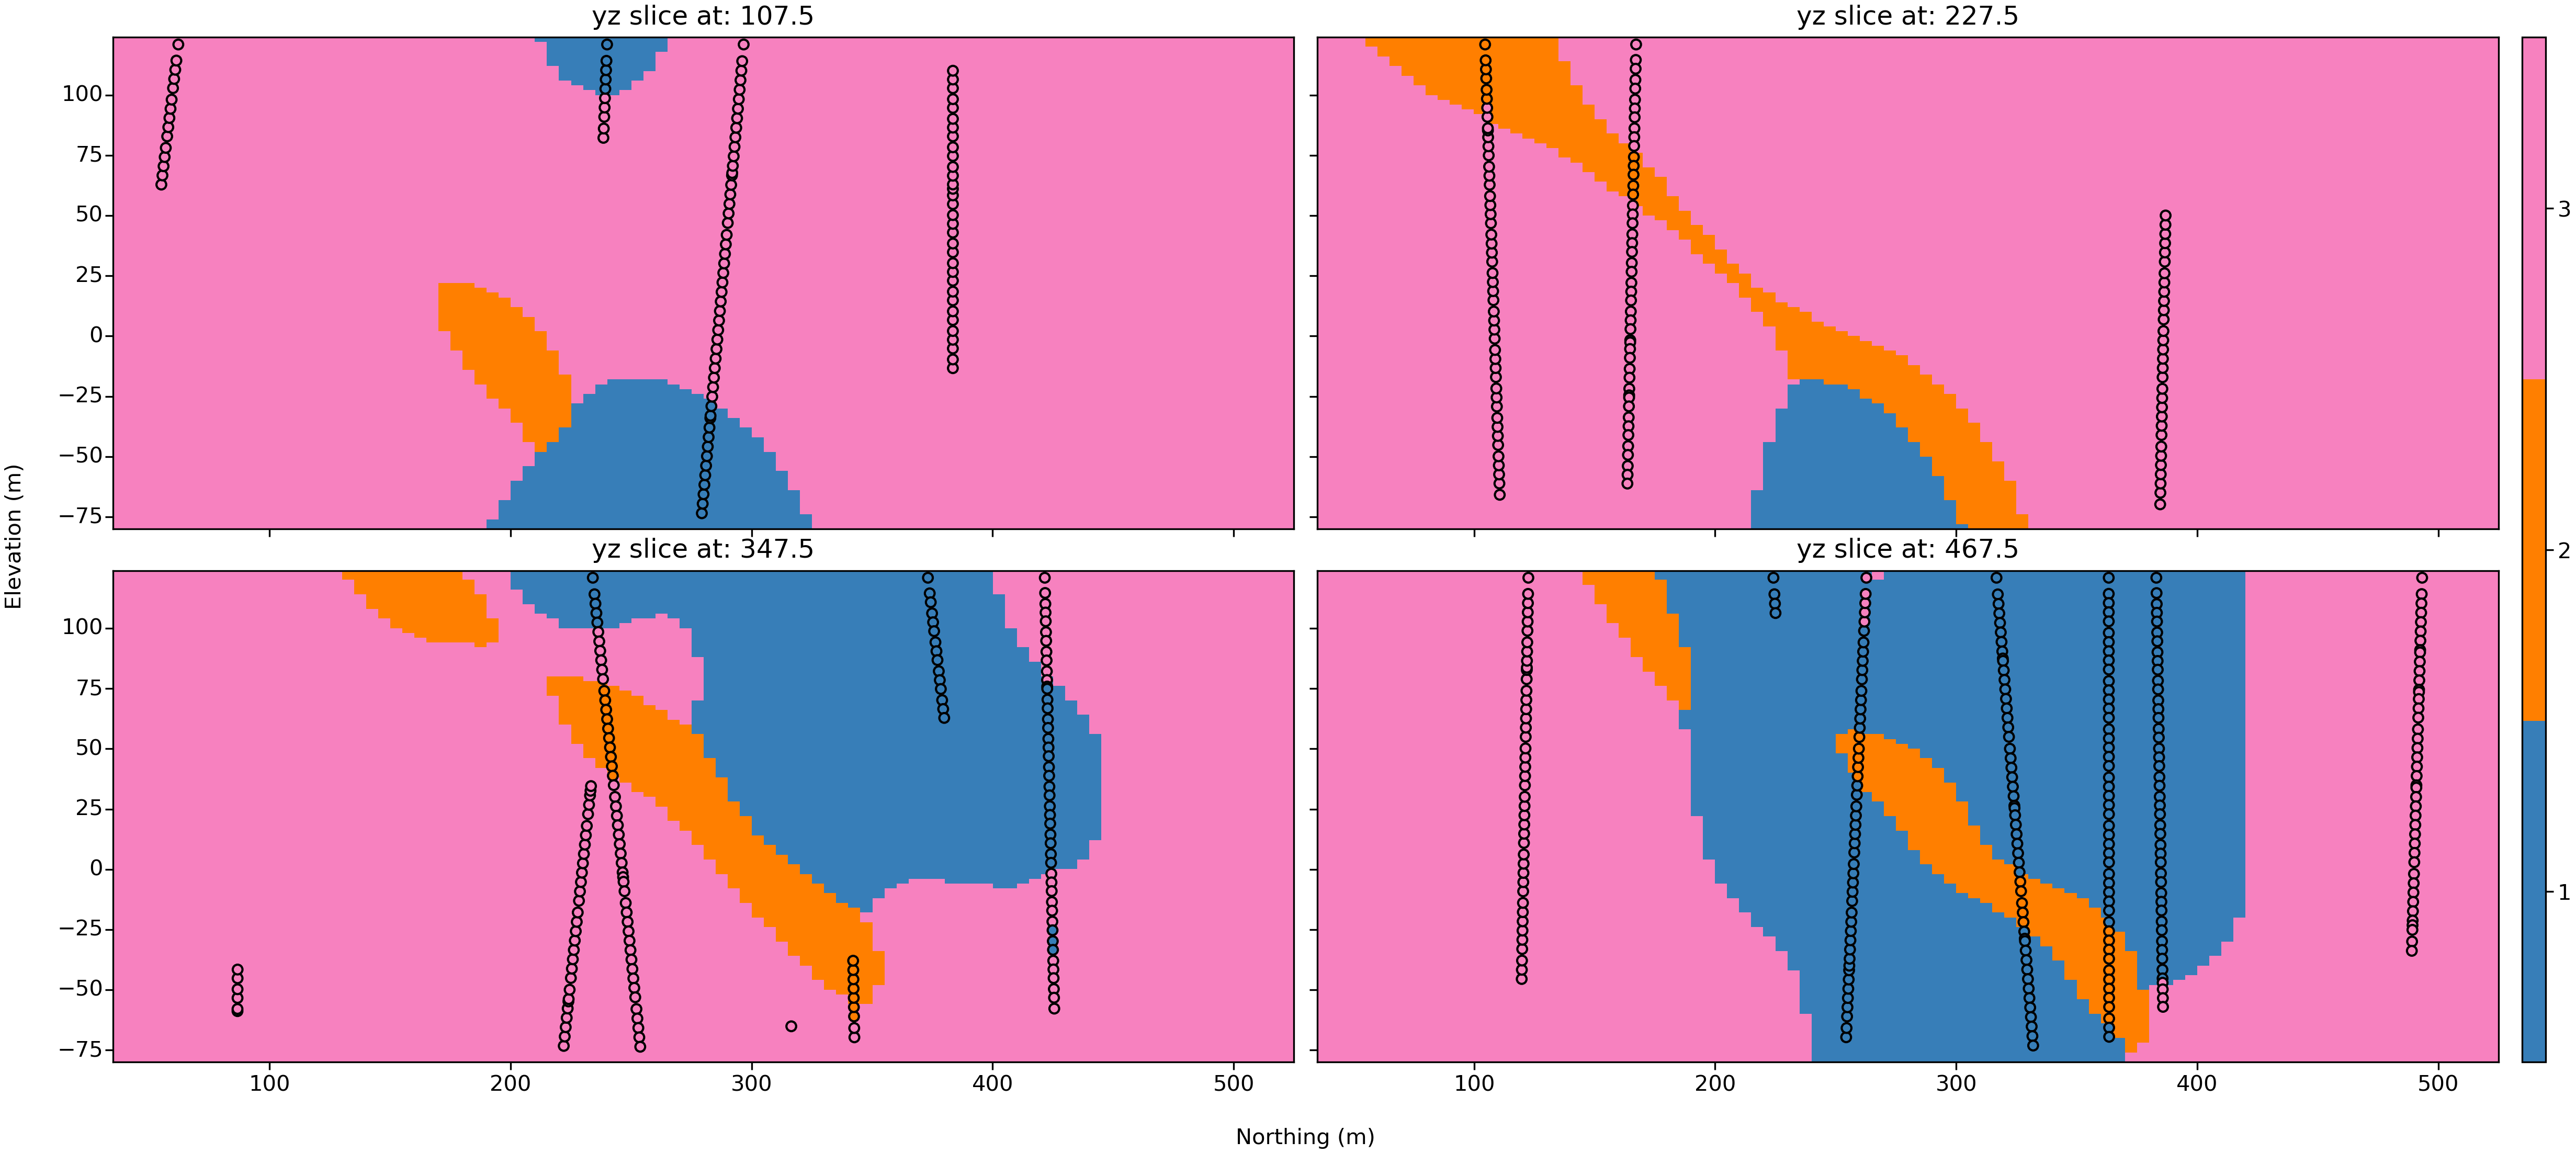
\includegraphics[width=.5\textwidth]{capitulo_2/anisofineryz.png}\label{<figure2>}}
\end{figure}
\note{Esse slide mostra 4 seções em xy e 4 seções em yz do modelo implicito multi categórico para o banco de dados do estudo de caso.
}
\end{frame}

\subsection{Incorporação da não estacionariedade de segunda ordem}

\begin{frame}{krigagem com anisotropia local variável}

\begin{figure}[H]
	\caption{\label{lva_krig_cartoon}Esquema mostrando os vetores de anisotropia local para cada nó do \textit{grid}.}
	\begin{center}
		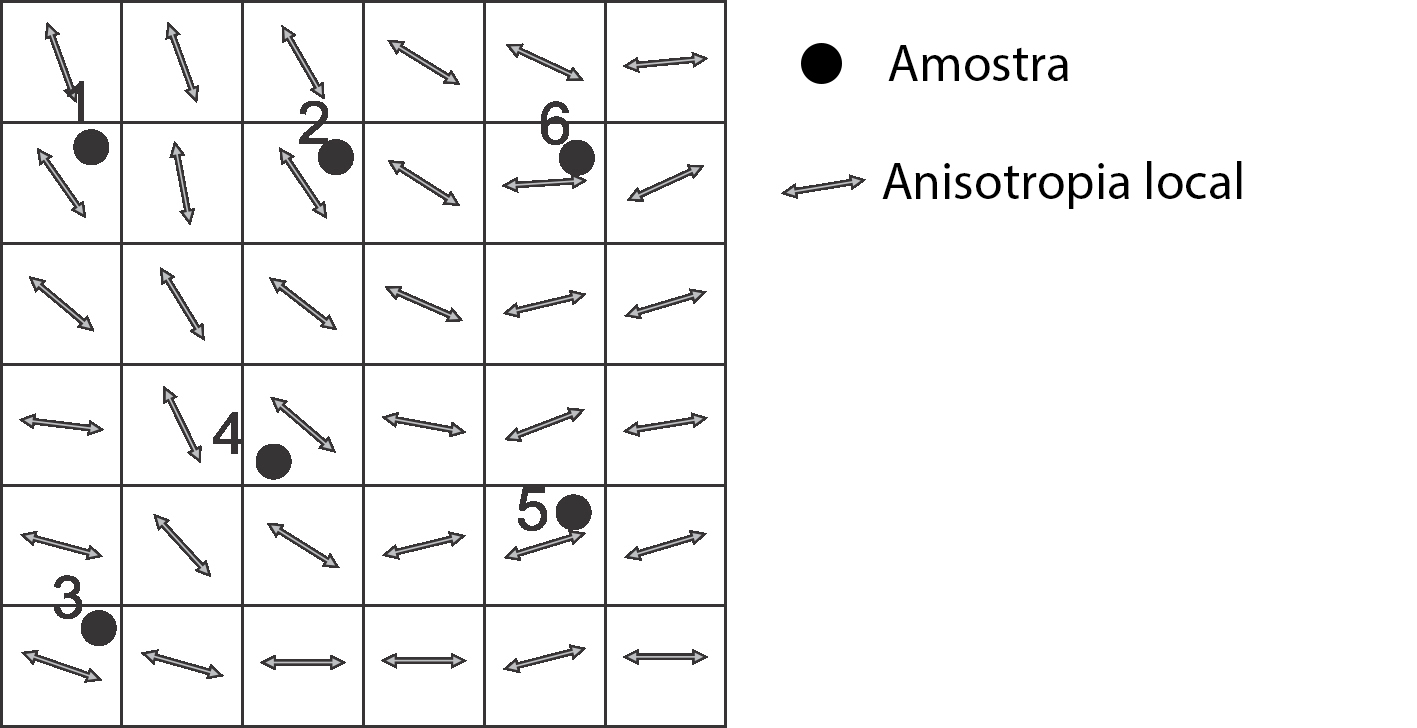
\includegraphics[width=0.8\textwidth]{capitulo_2/lvakrig1.jpg}
	\end{center}
	%\legend{Fonte: \citeonline{martin2017implicitmodeling}}
\end{figure}
	\note{Corpos geológicos podem ser bastante complexos E modelá-los considerando estacionariedade de segunda ordem, quer dizer, a função de covariância é estaciária, então a mesma anisotropia vale para toda região, pode ser muito restritivo.
		
		Uma alternativa é interpolar as distâncias por krigagem com anisotropia local variável, nesse método, para cada bloco a anisotropia local é derivada, então as distâncias são interpoladas por krigagem ordinária. Esse método pode demandar bastante esforço computacional já que em cada bloco a anistropia local deve ser calculada. }
\end{frame}

\begin{frame}
	\begin{figure}[H] 
		\caption{Iso superfície para a categoria 1 extraída de um modelo implícita gerado por krigagem com anisotropia local variável mostrando os vetores.} \label{lva_krig}
		\centering
		\subfloat[][Todos os vetores de anisotropia local]{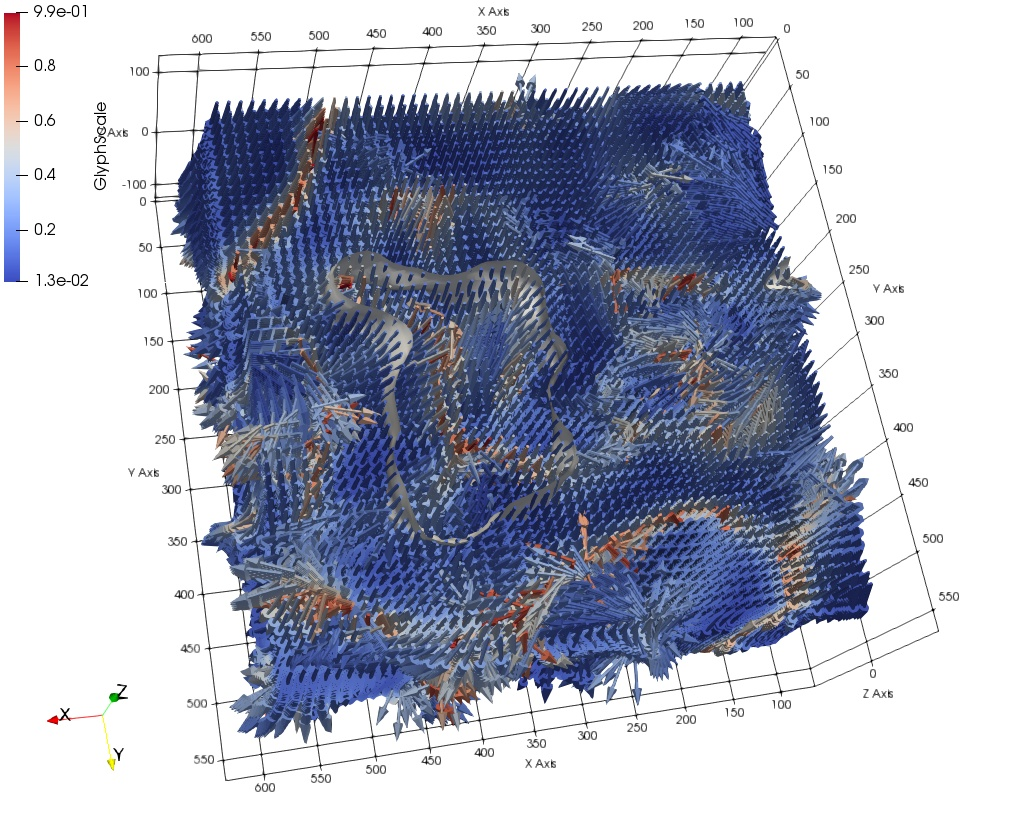
\includegraphics[width=.5\textwidth]{capitulo_2/lva_krig.jpeg}\label{<figure1>}}
		\subfloat[][Um vetor a cada 100.000 blocos]{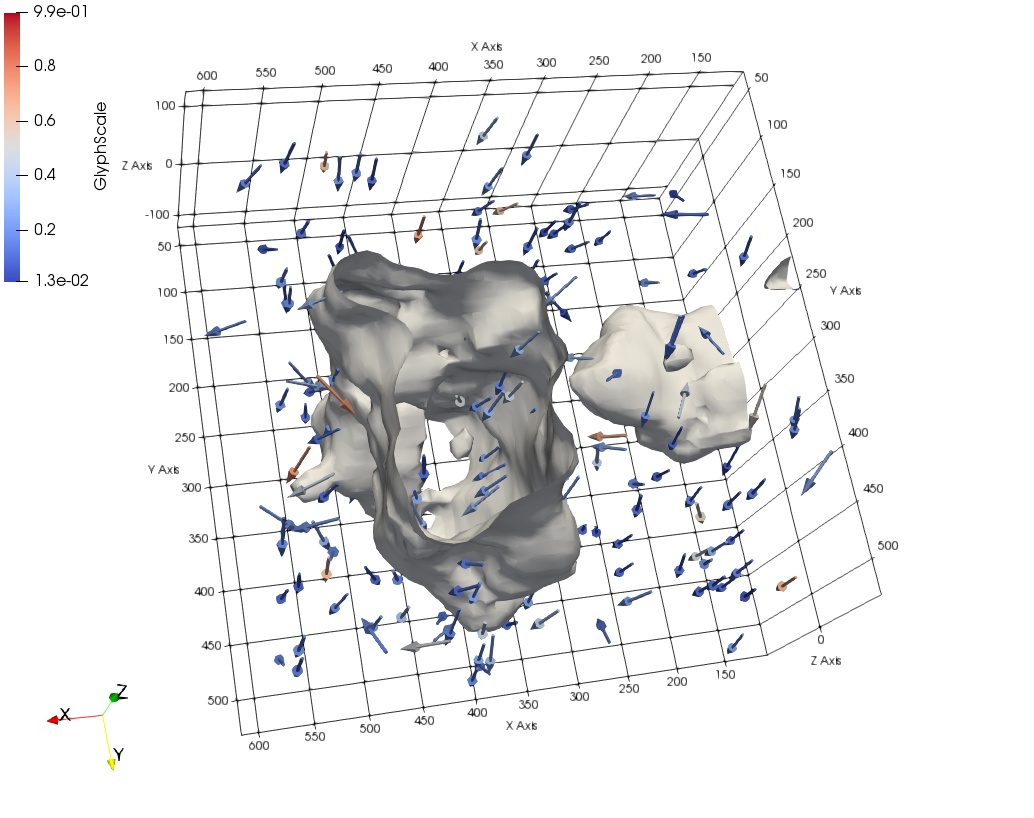
\includegraphics[width=.5\textwidth]{capitulo_2/lva_krig_100000.jpeg}\label{<figure2>}}
	\end{figure}
\note{Esse slide mostra os vetores de anostropia local em todos os um milhão de blocos do grid fino e a iso superfície extraída para a categoria 1, e ao lado mostrando um vetor a cada 10.000 blocos.}
\end{frame}

\begin{frame}{Funções de bases radiais com anisotropia local variável}
	\begin{figure}[H]
		\caption{\label{lva_rbf+cartoon} Esquema mostrando os vetores de anisotropia local para cada centro de partição.}
		\begin{center}
			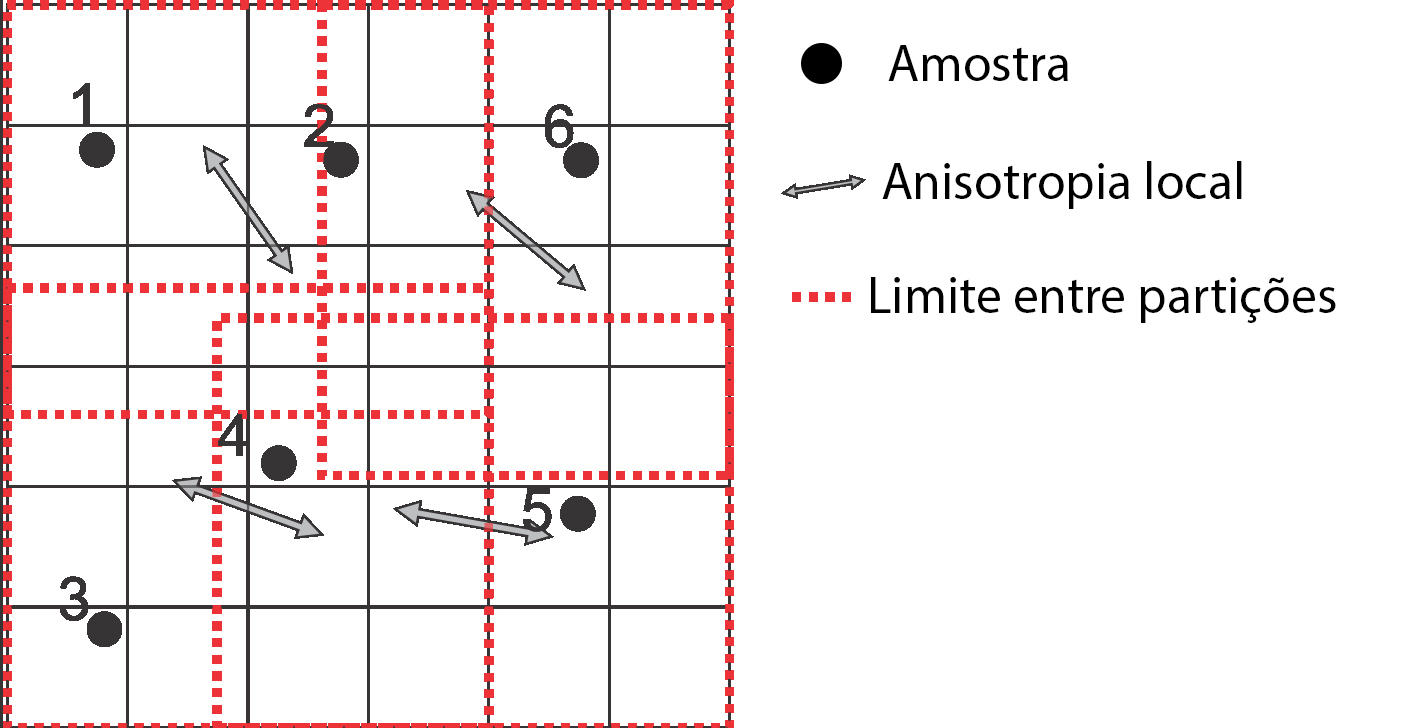
\includegraphics[width=0.8\textwidth]{capitulo_2/lvarbf1.jpg}
		\end{center}
		%\legend{Fonte: \citeonline{martin2017implicitmodeling}}
	\end{figure}
\note{Pra o fluxo de trabalho usando RBF também é possível implementar não estacionariedade de segunda ordem, baseado no particionamento do domínio que eu mostrei alguns slides pra trás. Dessa forma, pra cada partição a anistropia local é derivada. Esse método demanda menos esforço computacional, já que os vetores de anisotropia não precisam ser calculados para cada bloco.}
\end{frame}

\begin{frame}{Funções de bases radiais com anisotropia local variável}
	\begin{figure}[H]
		\caption{\label{rbf_iterref}Iso superfície para a categoria 1 extraída de um modelo implícita gerado por krigagem com anisotropia local variável mostrando os vetores.}
		\begin{center}
			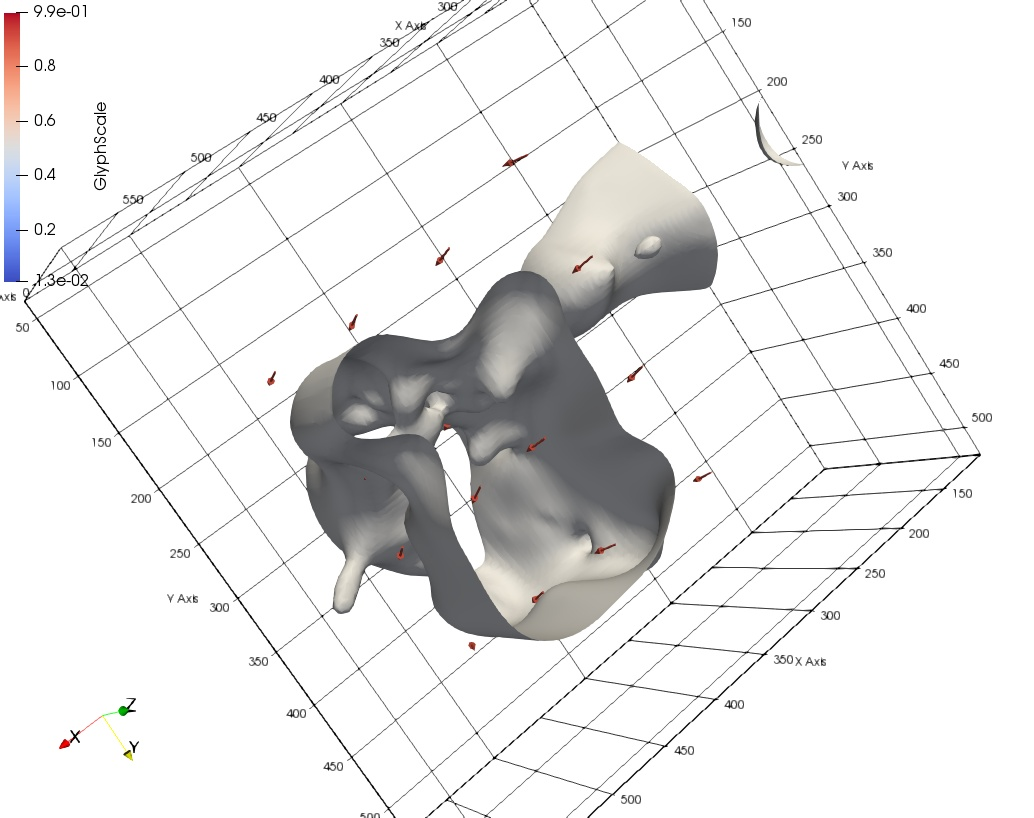
\includegraphics[width=0.5\textwidth]{capitulo_2/rbf_iterref.jpeg}
		\end{center}
		%\legend{Fonte: Modificado de \citeonline{silvageostatlessons}}
	\end{figure}
\note{Esse slide mostra os vetores de anostropia local para cada partição e a iso superfície extraída para a categoria 1.
}
\end{frame}

\subsubsection{Refinamento iterativo}

\begin{frame}{Refinamento iterativo}

Extrair orientações locais de um modelo criado com anisotropia global e utilizar essas orientações em uma nova interpolação não estacionária resulta em um modelo geológico mais refinado.

	\begin{figure}[H]
		\caption{\label{iterref} Esquema mostrando etapas usando o refinamento iterativo para funções de bases radiais.}
		\begin{center}
			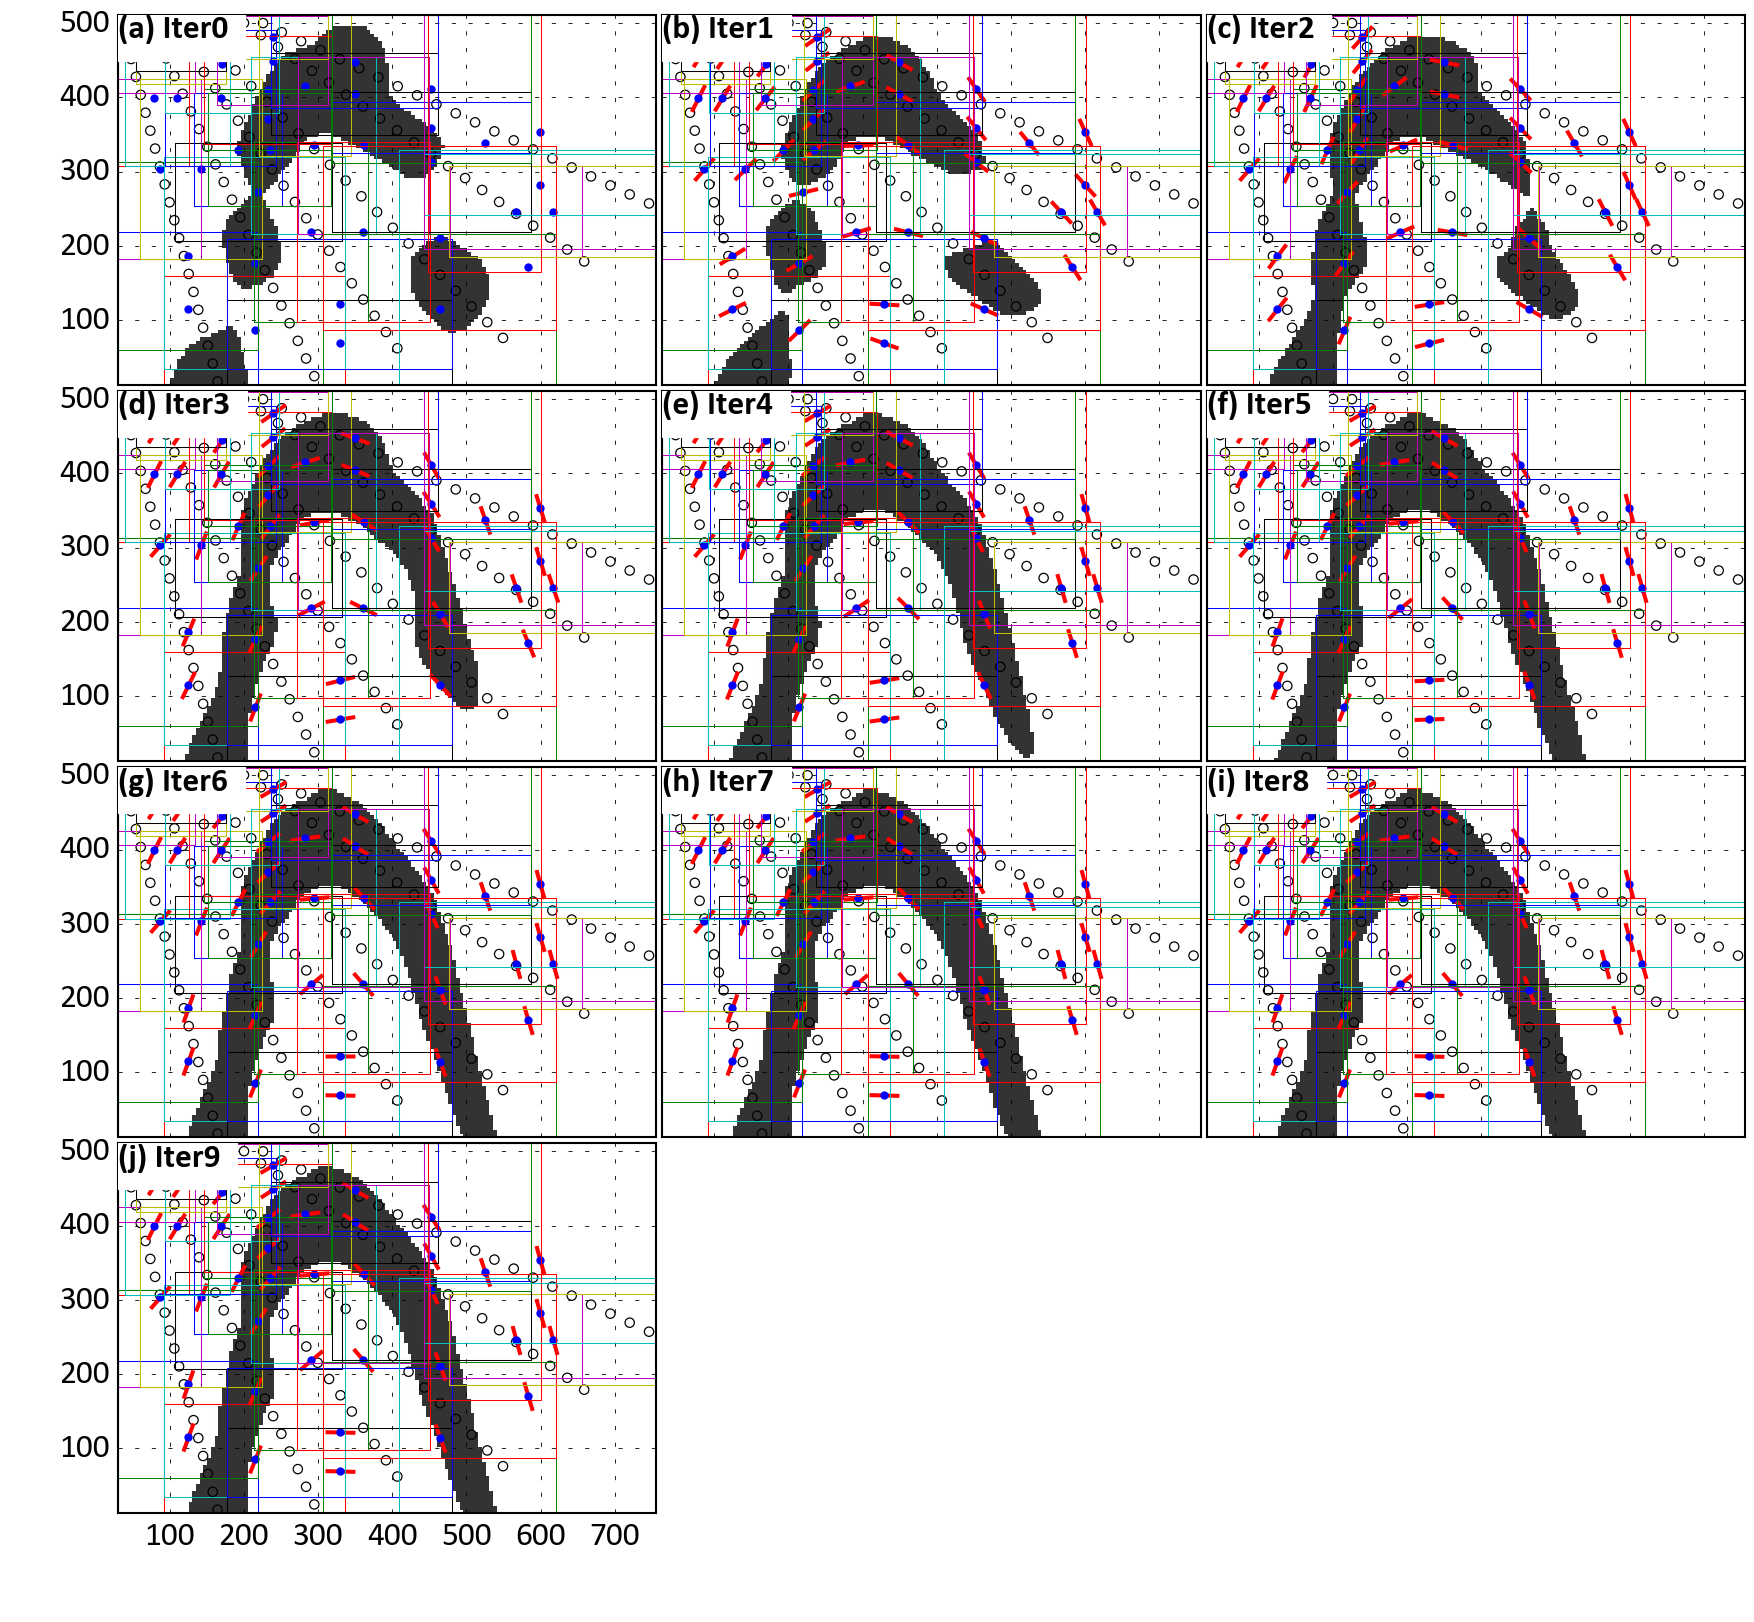
\includegraphics[width=0.37\textwidth]{capitulo_2/iterref.jpg}
		\end{center}
		%\legend{Fonte: \citeonline{martin2017implicitmodeling}}
	\end{figure}
\note{Pra obter resultados melhores é possível derivar os vetores de anisotropia local, interpolar as distâncias usando essa anisotropia local, então a partir das distâncias interpoladas, derivar novamente a anisotropia local e interpolar novamente, esse processo iterativo continua até que um cirtétio de parada pré estabelecido seja atingido.
	
	a imagem mostra uma dobra em que os flancos vão se definindo com as iterações. Apesar de ser um método iterativo, ele é bastante eficiente porque o critério de parada pode ser atingido em diferentes iterações em cada partição.}
\end{frame}

\subsection{Incorporação de informação secundária}

\begin{frame}{Incorporação de informação secundária}

\cite{manchuck_MLS} propõe o uso de uma regressão linear local para integrar modelagem geológica implícita e explicita.

	\begin{figure}[H]
		\caption{Modelo geológico híbrido criado a partir de furos de sondagem e seções interpretadas.}\label{mls_model}
			\subfloat[][Seção mostrando furos e seções interpretadas.]{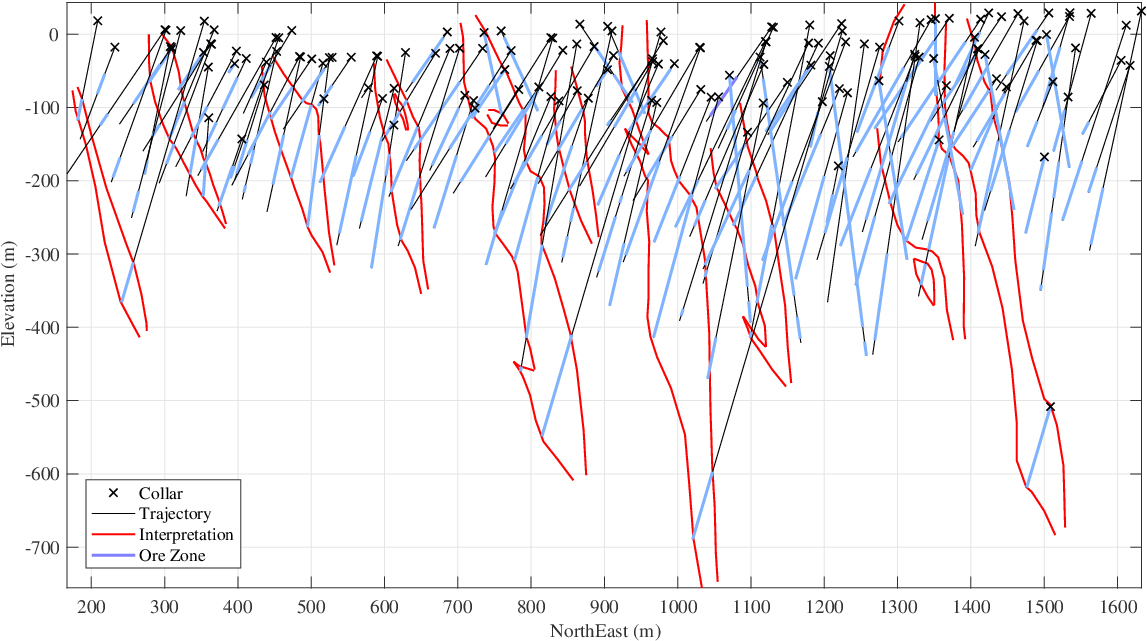
\includegraphics[width=0.5\textwidth]{capitulo_2/secoes.jpg}\label{a}}
			\subfloat[][Modelo implícito.]{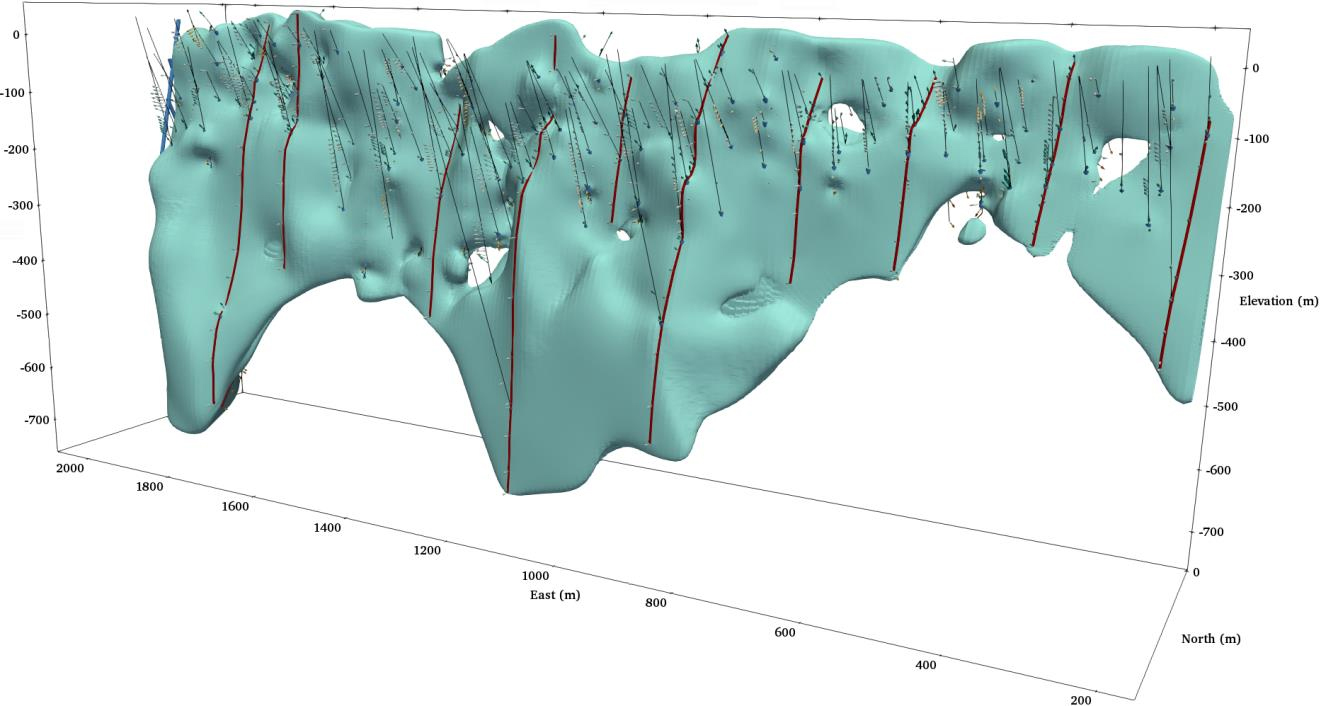
\includegraphics[width=0.5\textwidth]{capitulo_2/modelo_mls.jpg}\label{b}}
			%\legend{Fonte: \citeonline{manchuck_MLS}}
	\end{figure}
\note{Ainda no assunto interpolação, o jonh manchuck e o proferssor clayton desenvolveram uma metodologia para incorporar seções digitalizadas na modelagem implícita. Para isso as distancias mais seções digitalizadas devem ser interpoladas por mínimos quadrados móveis. Porém, o método ainda é recente e segundo os autores ainda apresenta alguns problemas operacionais.}
\end{frame}

\section{Avaliação da incerteza}

\subsection{Avaliação heurística da incerteza}

\begin{frame}{Avaliação heurística da incerteza}

Transformação das distâncias em probabilidades.
	\begin{equation}
	P(i(u)=k)=\frac{e^\frac{-d^*_k(u)}{\gamma}}{\sum_{k'=1}^{K}e^\frac{-d^*_k(u)}{\gamma}}
	\label{eq_softmax}
	\end{equation}
	
	\begin{figure}[H]
		\caption{\label{softmax_grafico}Distâncias estimadas em (a) e transformadas em probabilidades em (b) para um mesmo bloco, com cinco categorias.}
		\begin{center}
			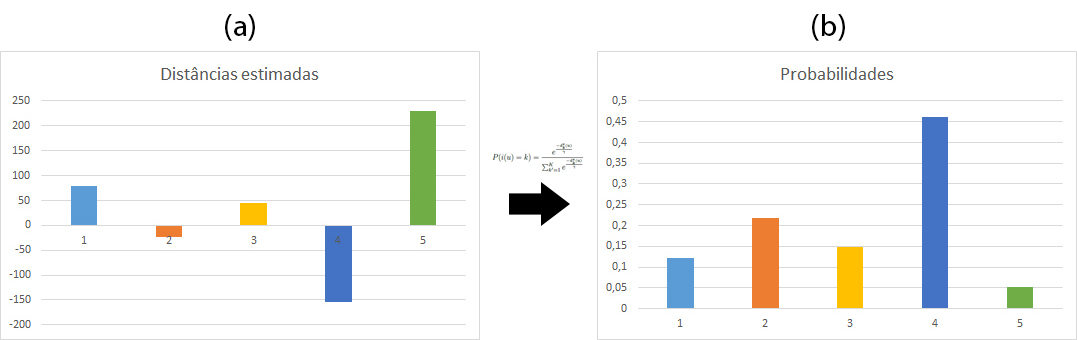
\includegraphics[width=0.7\textwidth]{capitulo_2/softmax_bars_final.jpg}
		\end{center}
		%\legend{Fonte: \citeonline{rolo_dissertacao}}
	\end{figure}
\note{Os próximos slides vão apresentar os métodos de avaliação de incerteza disponíveis na literatura e comentar um pouco sobre as características de cada um deles. 
	
	O método mais simples, é uma avaliação heirística da incerteza, porque não é baseado em múltiplas realizações. Consiste em transformar as distâncias em probabilidades. na equação para calcular a probabilidade da categoria k no local não amostrado i, o d* é a ditância estimada para a categoria k e gamma é um parametro que controla a incerteza. Quanto maior gamma maior a diferença entre as probabilidades calculadas. 
	
	o grafico de barras mostra as ditâncias assinaladas interpaladas para um bloco em particular, e ao lado as distâncias transformadas em probabilidades, quanto menor a distância, quanto mais negativa, maior a probabilidade. 
	
	Esse é um método bem simples, rápido e direto e funciona pra multiplas categorias simultâneas. Em contrapartida, a escolha do parâmetro gamma é subjetiva, alguns autores indicam que seja a maior distância estimada entre todas as categorias, e dependendo do gamma escolhido nem blocos co locados com amostras recebem prbabilidade 100 por cento.}
\end{frame}

\subsection{BOUNDSIM}

\begin{frame}{BOUNDSIM}

Krigagem simples com médias tomadas do histograma da média.

\begin{columns}
	\begin{column}{0.5\textwidth}
	\begin{figure}[H]
		\caption{\label{bs_df_1}Histograma do bootstrap espacial da média das distâncias assinaladas para a categoria 1.}
		\begin{center}
			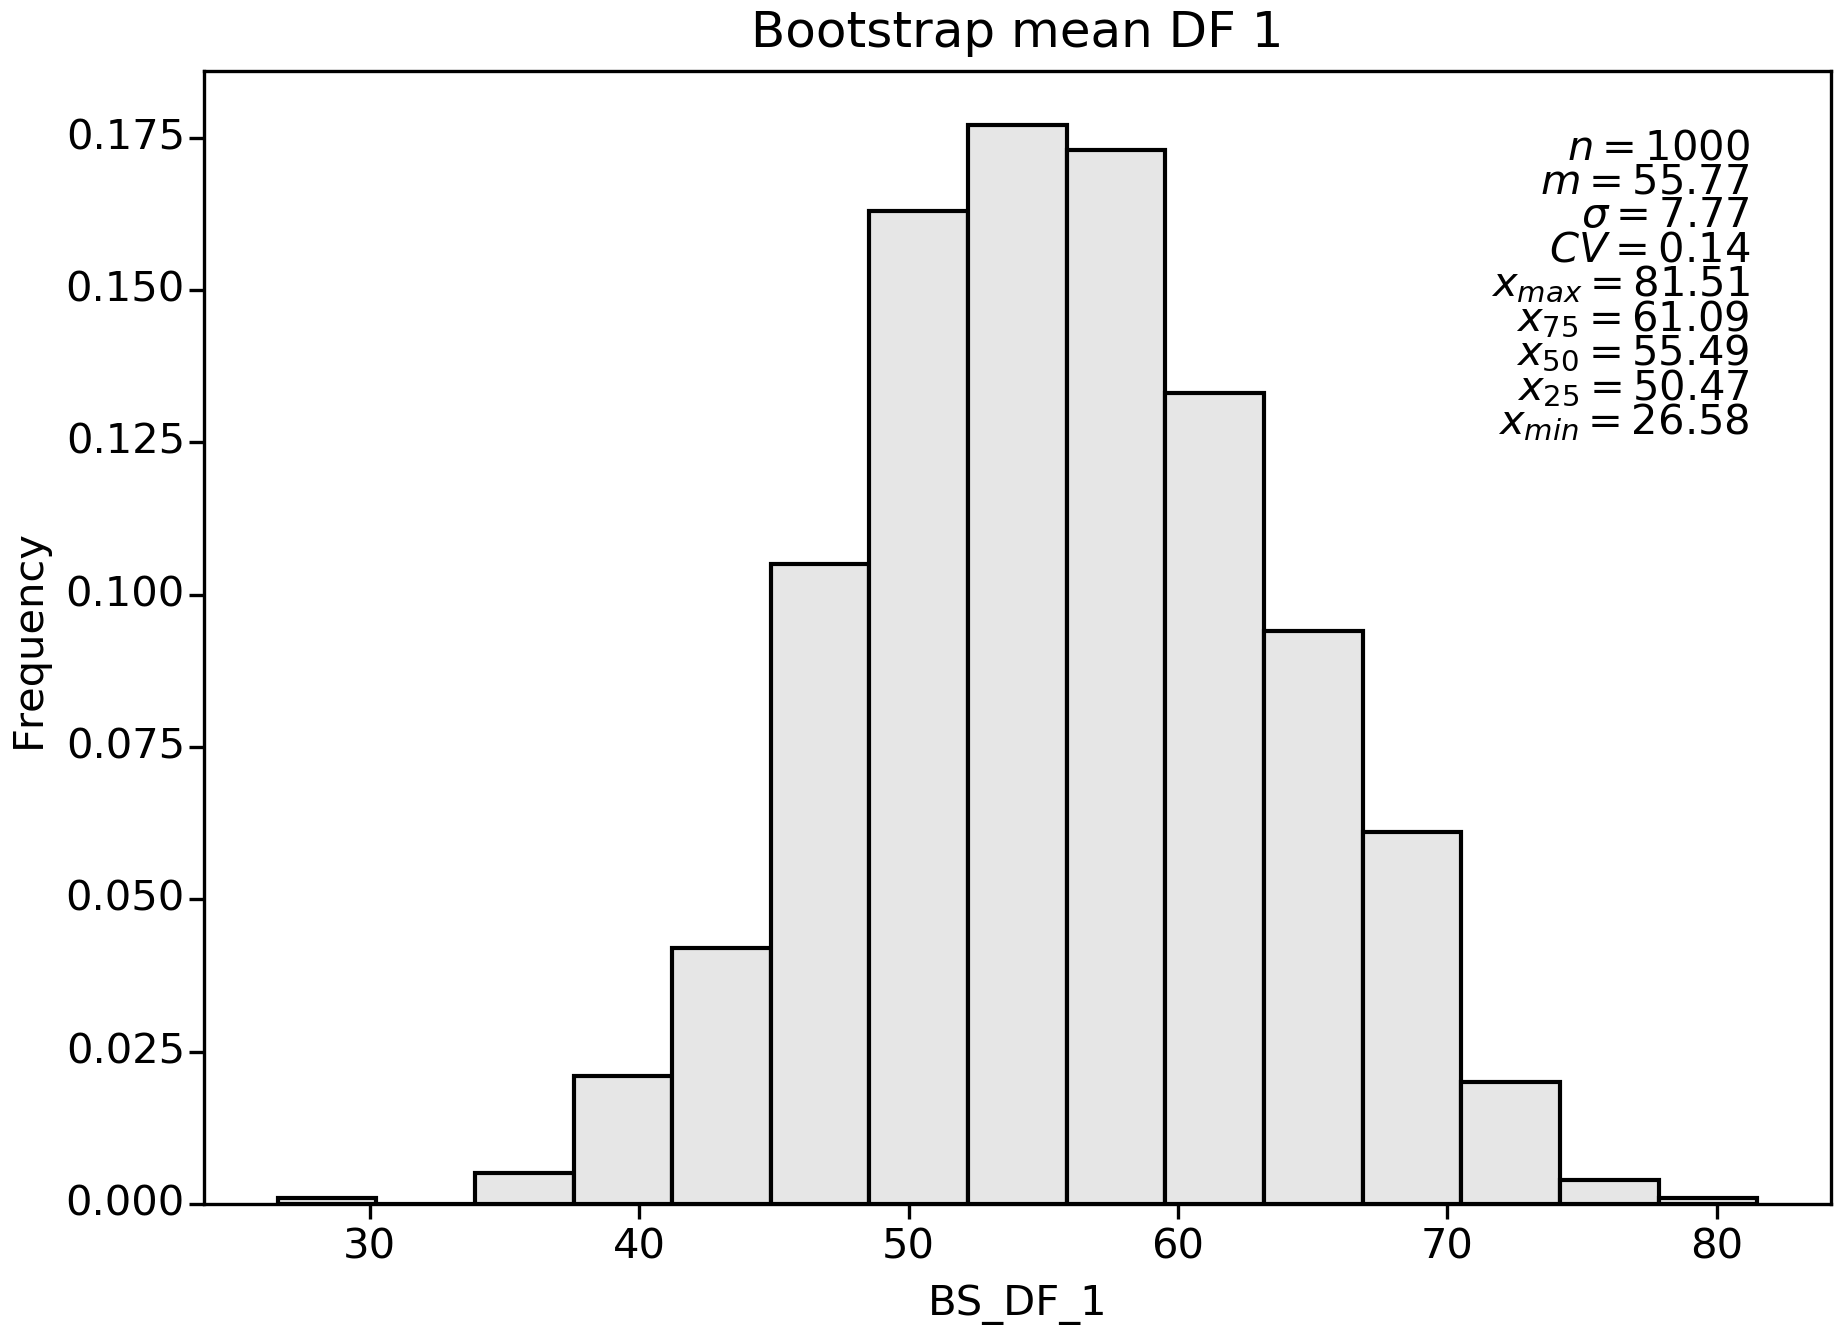
\includegraphics[width=\textwidth]{capitulo_2/BS_DF_1.png}
		\end{center}
		%\legend{Fonte: \citeonline{rolo_dissertacao}}
	\end{figure}
	\end{column}
	\begin{column}{0.5\textwidth}  %%<--- here
	\begin{table}[H]
			\begin{center}
					\begin{tabular}{lr}
					Percentil & \multicolumn{1}{l}{Blocos dentro} \\ \hline
					10 & 109886 \\
					50 & 110446 \\
					90 & 111069 \\ \hline
				\end{tabular}

			\end{center}
						%\caption{Blocos classificados como pertencentes à categoria 1.}\label{boundsim_table}
	\end{table}
	\end{column}
\end{columns}
\note{O próximo método, aumentando um pouco a complexidade, consiste, primeiramente em realizar um bootstrap espacial da média da distância assinalada, o bootstrap espacial só leva em consideração amostras não correlacionadas. Assim eu tenho um histograma da média, que é mostrado no slide, a partir desse histograma eu posso tomar valores, como o p10, p50 e p90 por exemplo, e intepolar as ditâncias assinaladas por krigagem simples, usando esses valores tomados como média. Em tese, eu poderia extrair diferentes iso superfícies zero dos modelos interpolados com diferentes médias. 

Porém na prática, dependendo da configuração espacial das amostras a krigagem simples não é sensível à media, para a categoria do banco de dados do estudo de caso, a diferença de volume entre as isosuperficies extraidas do modelo p10 e p90 é menor que 1por cento. O método não avalia adequadamente a incerteza, além disso, trabalha com uma categoria por vez, na presença de múltiplos domínios é necessário uma abordagem heirárquica.}
\end{frame}

\subsection{Simulação direta das distâncias assinaladas}

\begin{frame}{Simulação direta das distâncias assinaladas}

Simulação direta e classificação dos blocos baseada na menor distância simulada.

O primeiro passo é o cálculo do coeficiente U:

\begin{equation}\label{u_eq}
U(u)=\frac{max\{D_{min}\}-min\{d^*_k(u)\}^K_{k=1}}{max\{D_{min}\}-min\{D_{min}\}}
\end{equation}

Onde:

\begin{equation}
D_{min}=\{min\{d^*_k(u_1)\},...,\{min\{d^*_k(u_n)\}^K_{k=1}\}
\end{equation}

E $d^*_k(u)$ é a distância estimada no local u para a categoria k.

\note{O próximo método é a primeira ideia que surge em mente em relação à avaliação de incerteza de modelos geológicos implícitos: a simulação direta das distâncias. 
	
	O primeiro passo é calcular um coeficiente U de incerteza. Antes de qualquer coisa eu preciso criar uma lista com as menors distâncias interpoaldas em cada bloco. Então pra cada bloco eu eu subtraio do valor maximo dessa lista a menor distância estimada naquele bloco. O denominador é pra estandardizar entre 0 e 1.}
\end{frame}

\begin{frame}{Simulação direta das distâncias assinaladas}
	\begin{figure}[H]
		\caption{\label{u_fig}Coeficiente U calculado para todos os nós do \textit{grid}.}
		\begin{center}
			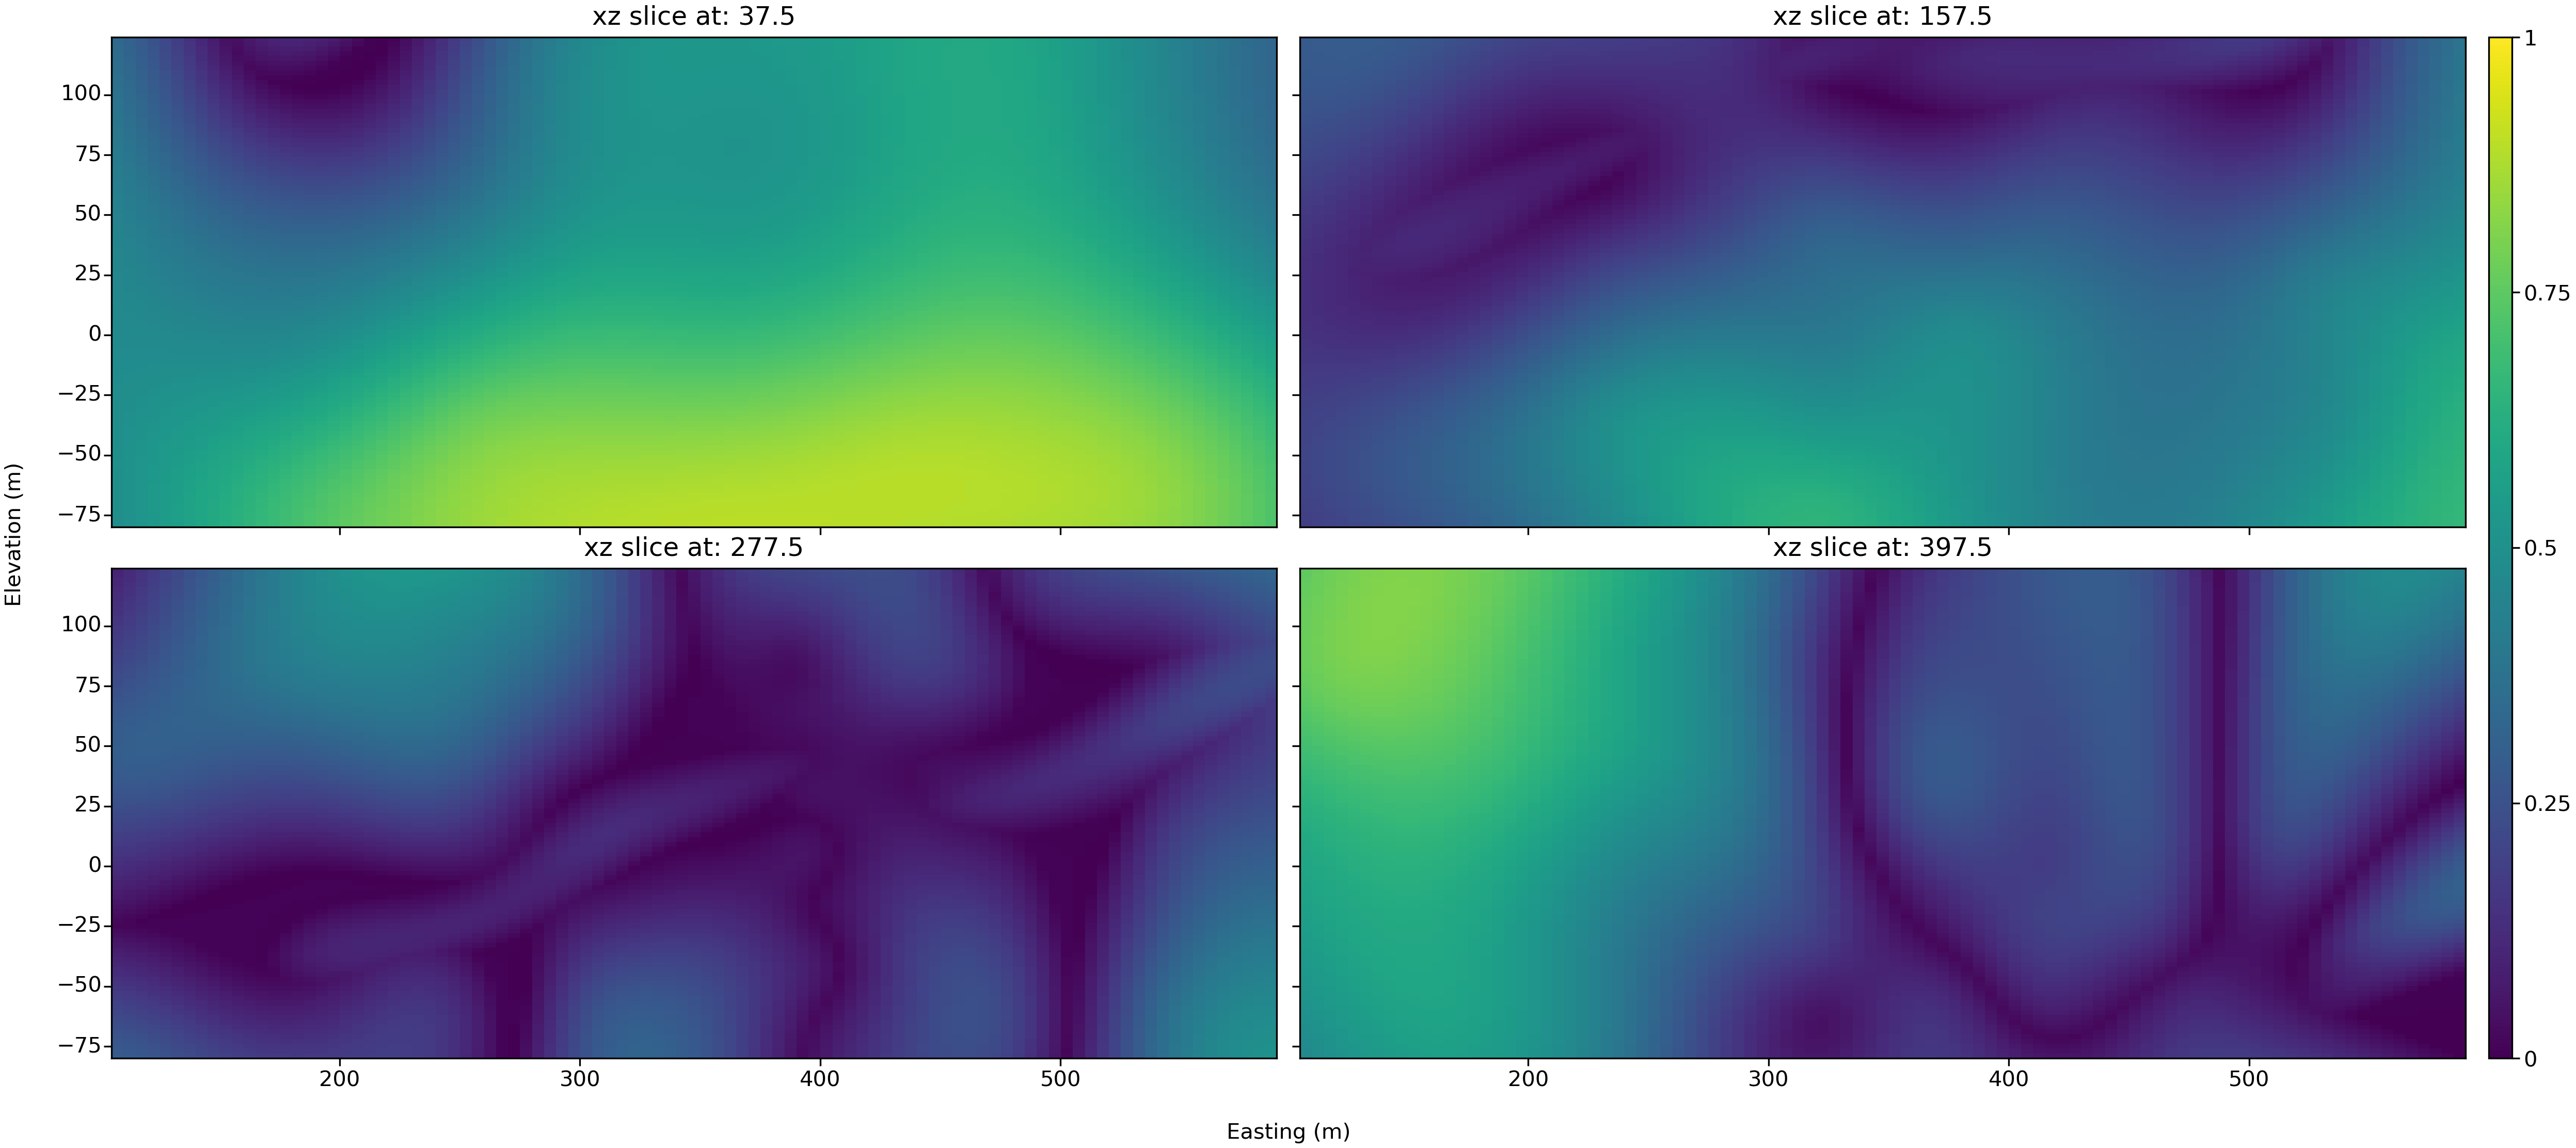
\includegraphics[width=0.8\textwidth]{capitulo_2/u_coef.png}
		\end{center}
		%\legend{Fonte: \citeonline{rolo_dissertacao}}
	\end{figure}
\note{Esse slide mostra 4 seções verticais do coeficiente U, esse coeficiente basicamente delinea os contatos, ele é mais próximo de 1 onde há mais incerteza e mais próximo de zero onde não há.
	
	Agora é necessário fazer uma truncagem entre 0 e 1 no coeficiente U pra delimitar uma zona e incerteza, quanto mais perto de 1 mais estreita é a zona de incerteza. As distâncias não precisam ser simuladas em todos os nós do grid, porque no interior dos domínios não há incerteza.}
\end{frame}

\begin{frame}{Simulação direta das distâncias assinaladas}

Simulação das distâncias na zona de incerteza:

	\begin{figure}[H] 
		\caption{Distâncias simuladas na zona de incerteza para as categorias do banco de dados.} \label{dist_sim_u}
		\centering
		\subfloat[][Categoria 1]{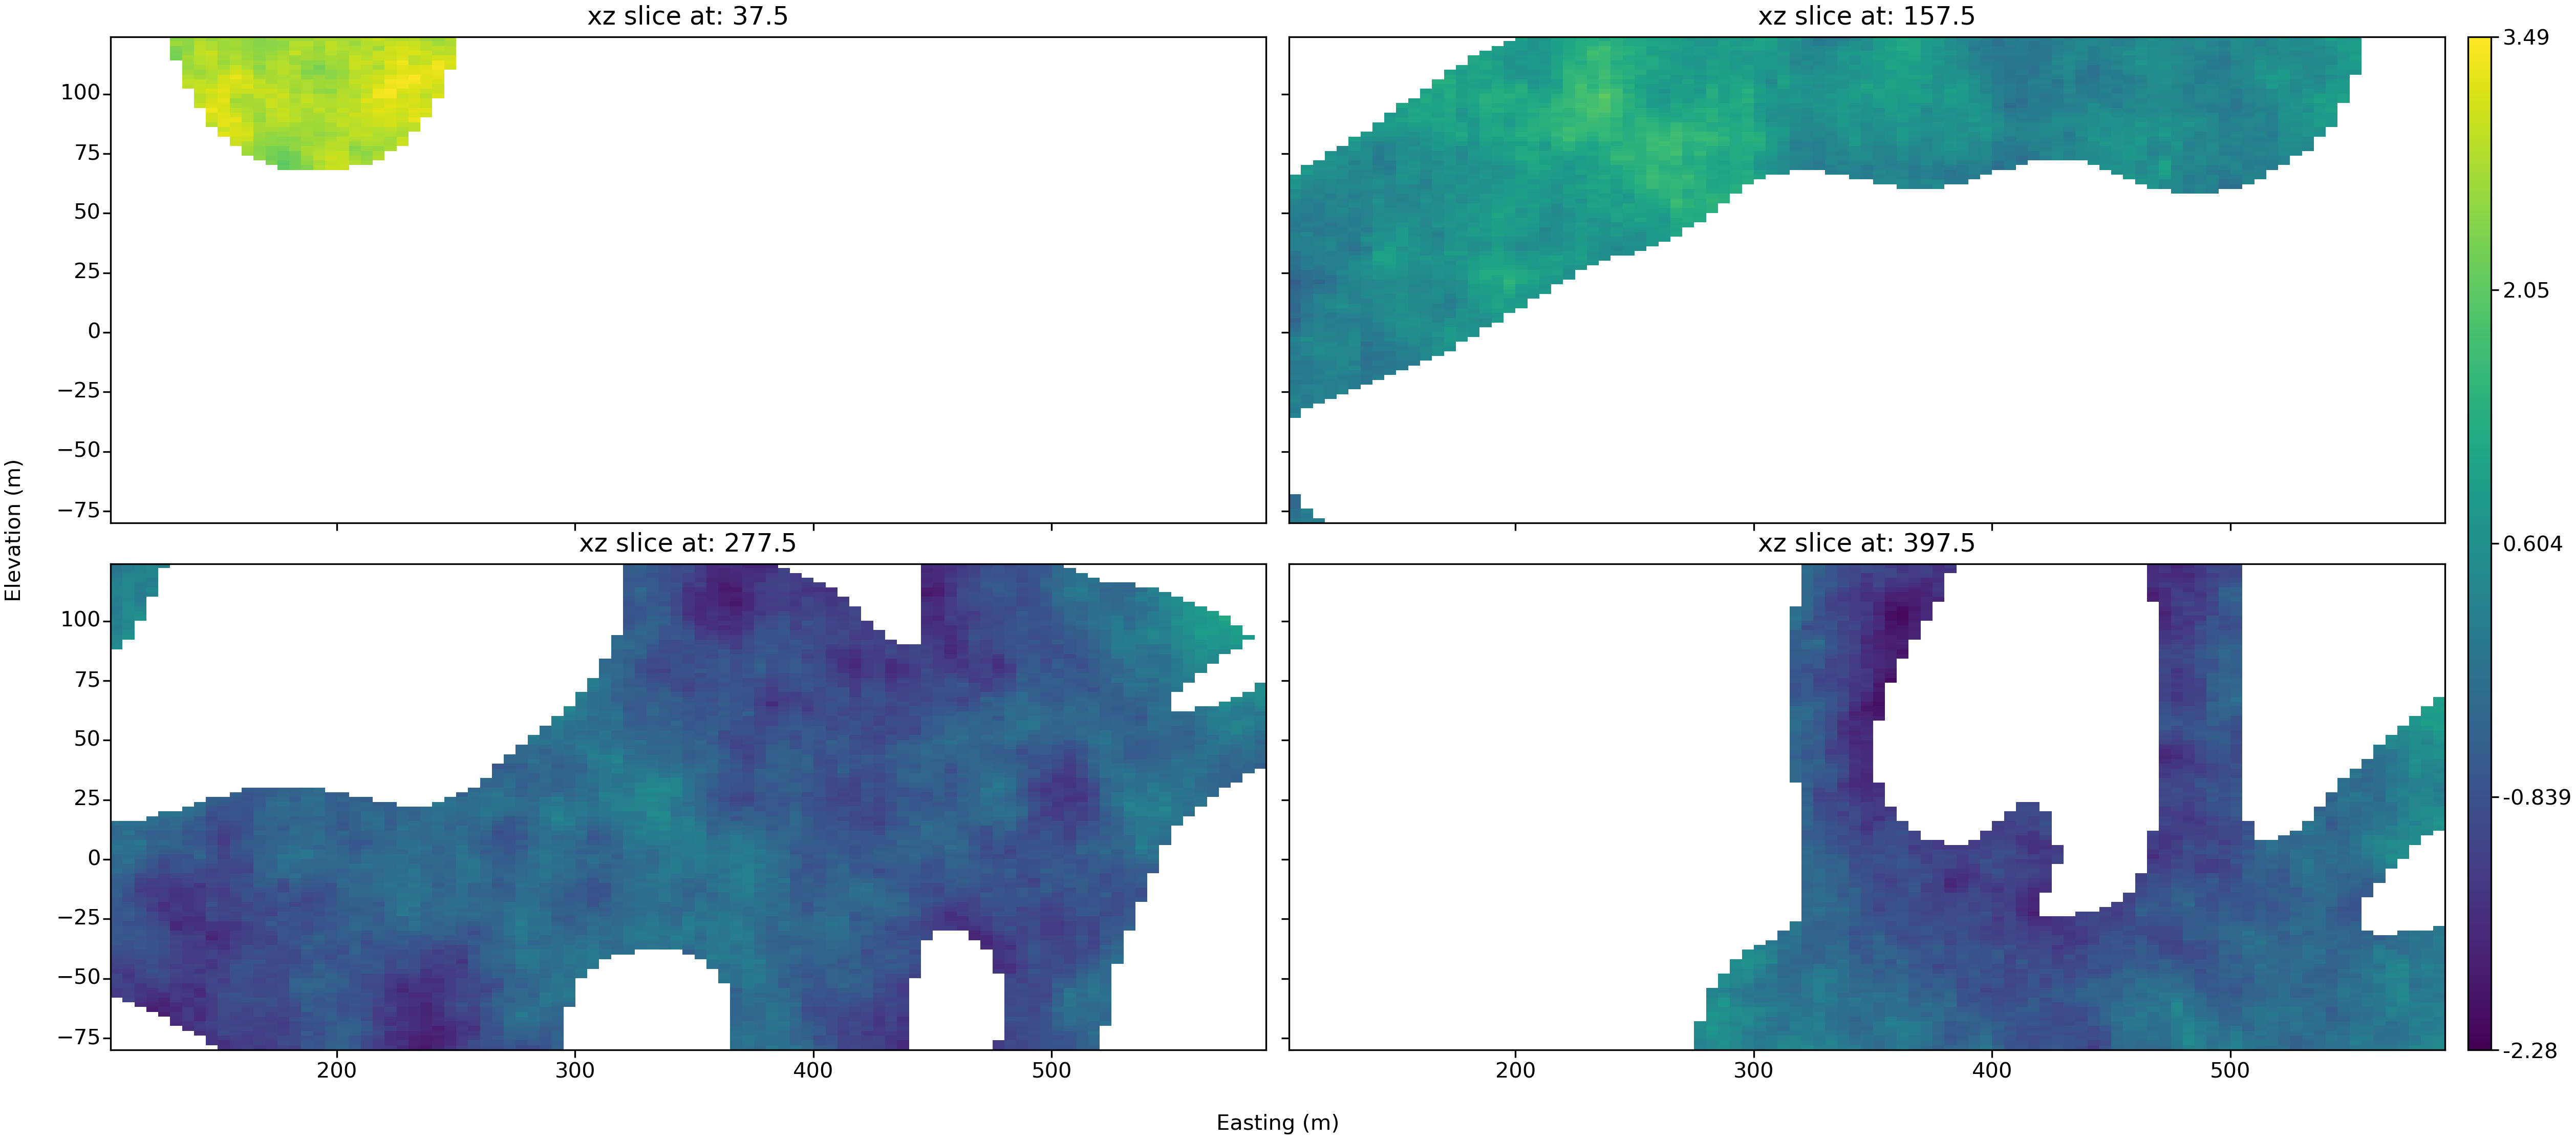
\includegraphics[width=.35\textwidth]{capitulo_2/Ucutoff1.png}\label{<figure1>}}
		\subfloat[][Categoria 2]{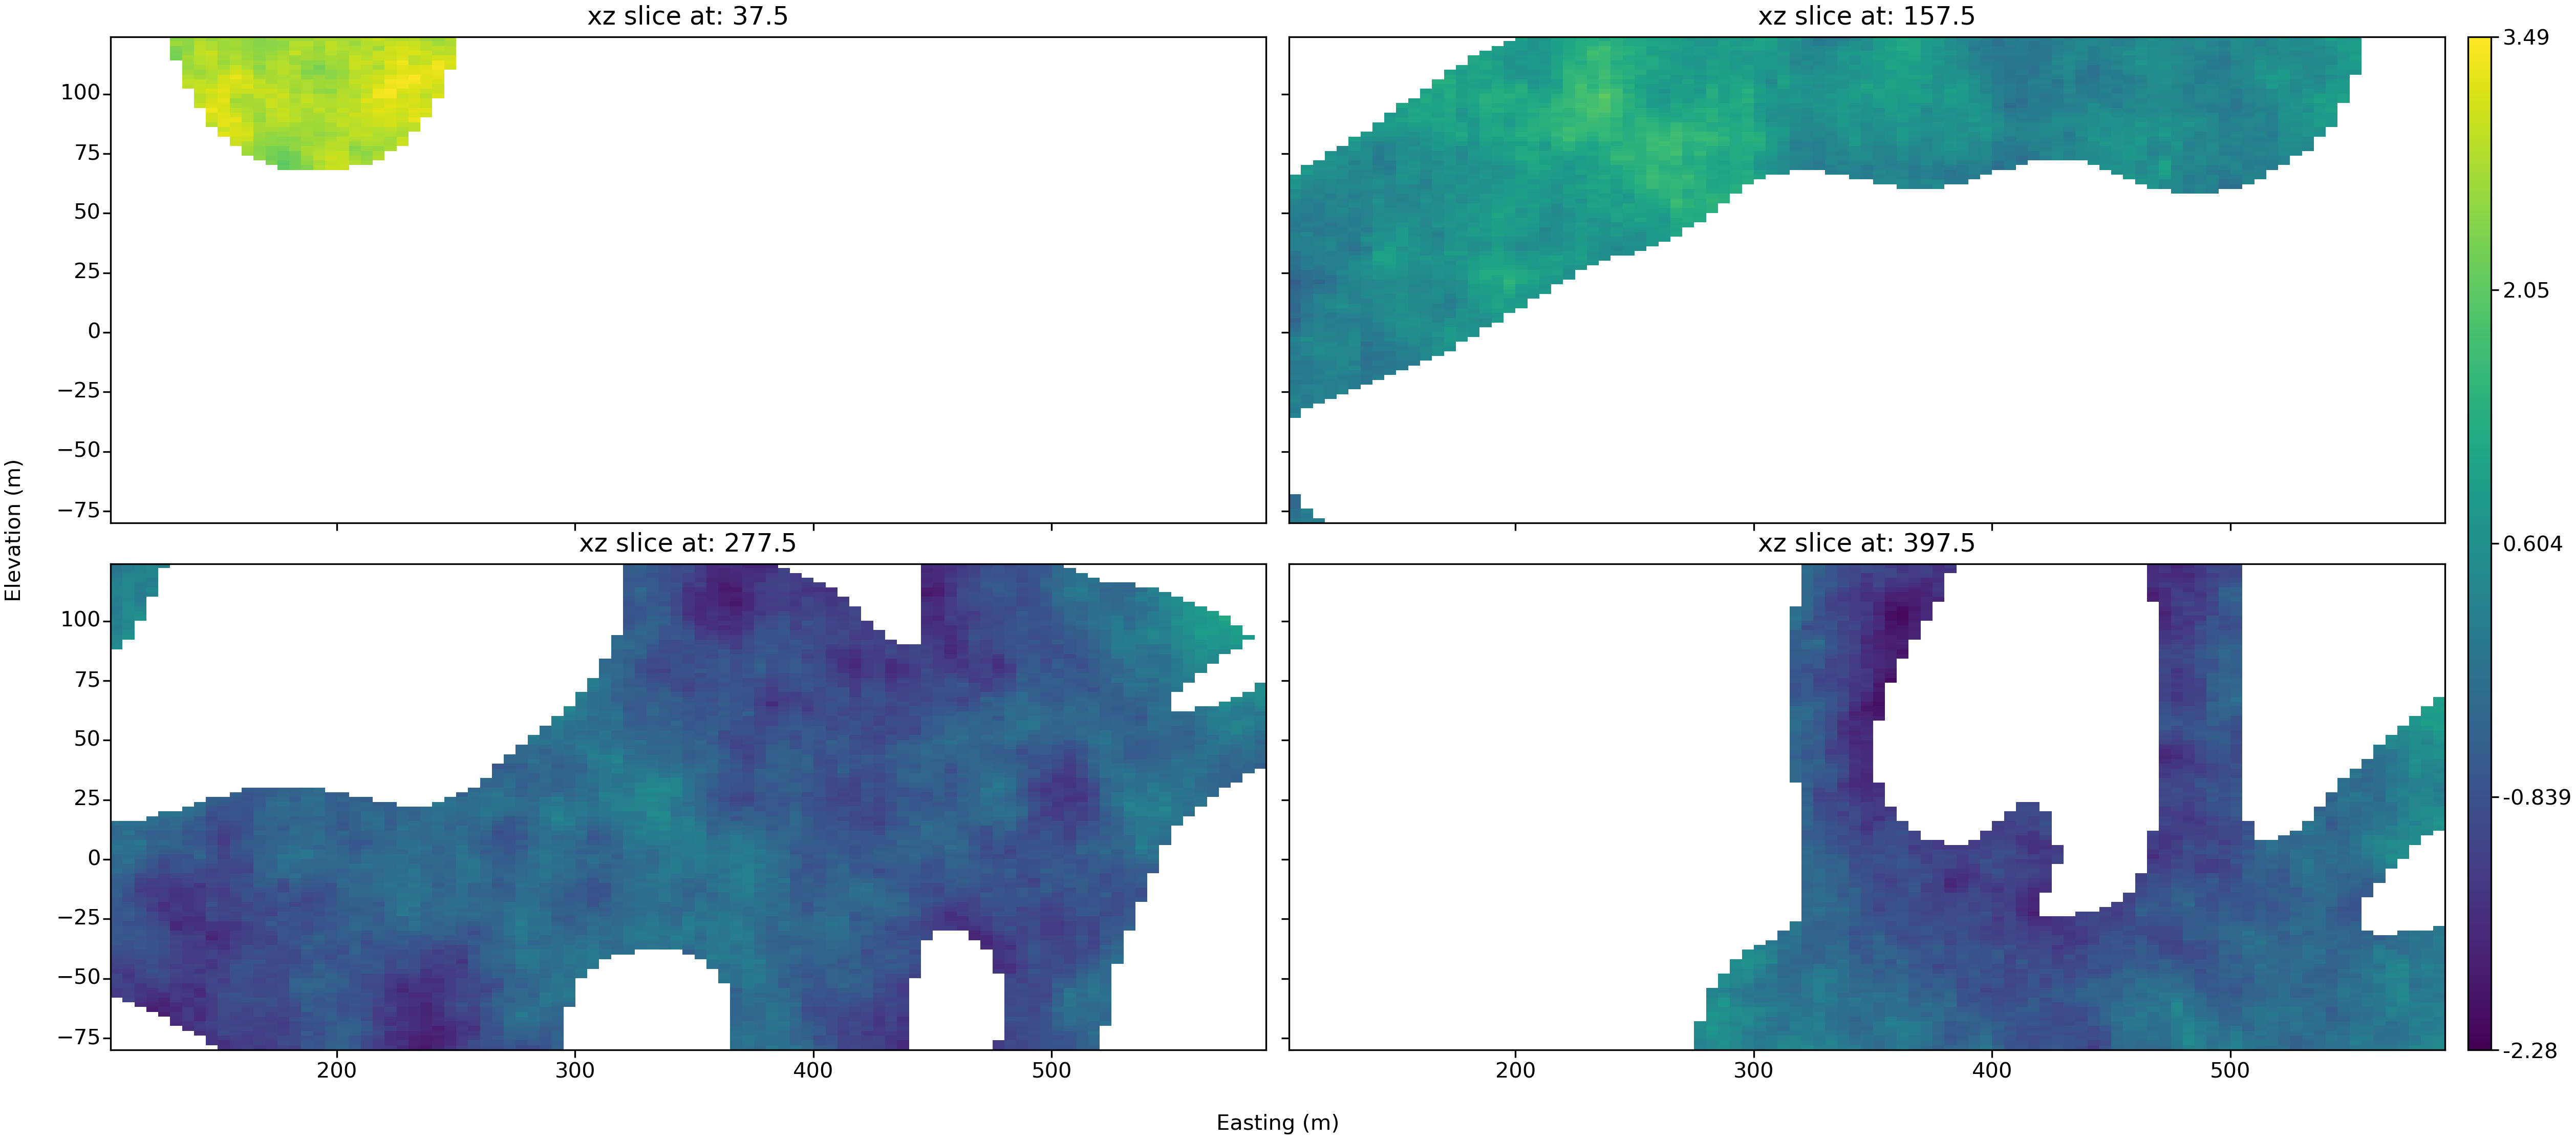
\includegraphics[width=.35\textwidth]{capitulo_2/Ucutoff2.png}\label{<figure2>}}
		\subfloat[][Categoria 3]{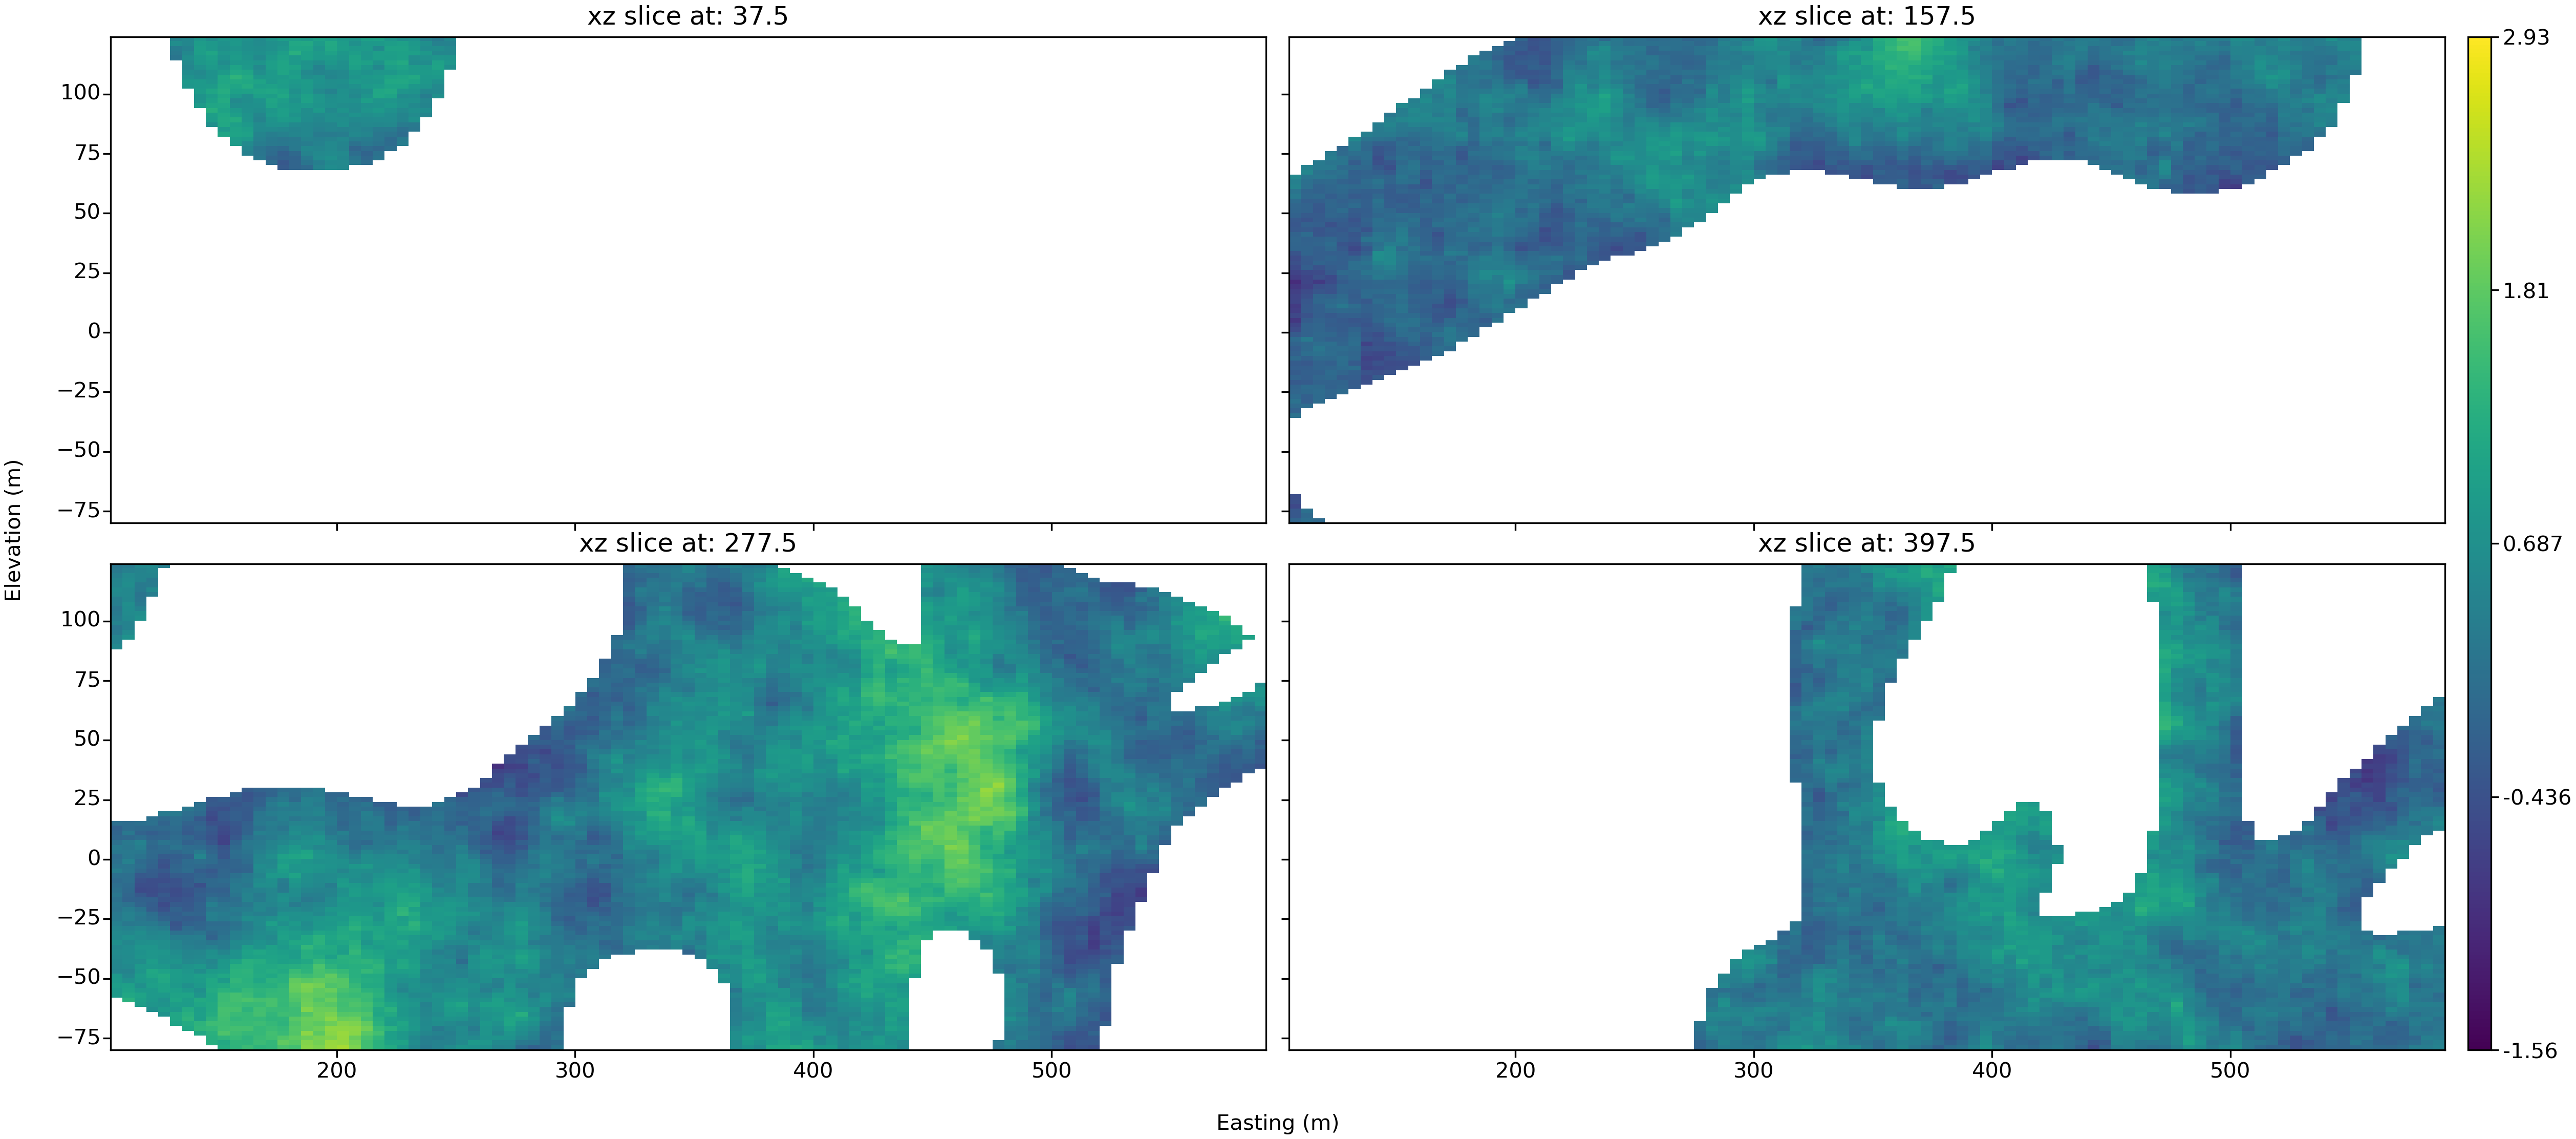
\includegraphics[width=.35\textwidth]{capitulo_2/ucutoff3.png}\label{<figure2>}}
	\end{figure}
\note{Esse slide mostra uma realização das distâncias simuladas na zona de incerteza pra cada uma das litologias do banco de dados.
	
	Os blocos fora da zona de incerteza ficam congelados, e recebem a a categoria respons;avel pela menor ditânca estimada, enquanto os blocos na zona de incerteza recebem a categoria responsável pela menor distância simulada, em cada realização.}
\end{frame}

\begin{frame}{Simulação direta das distâncias assinaladas}

Classificação dos blocos.

	\begin{figure}[H]
		\caption{Diferentes realizações do modelo geológico.} 
		\label{dif_real}
			\subfloat[][Realização 1]{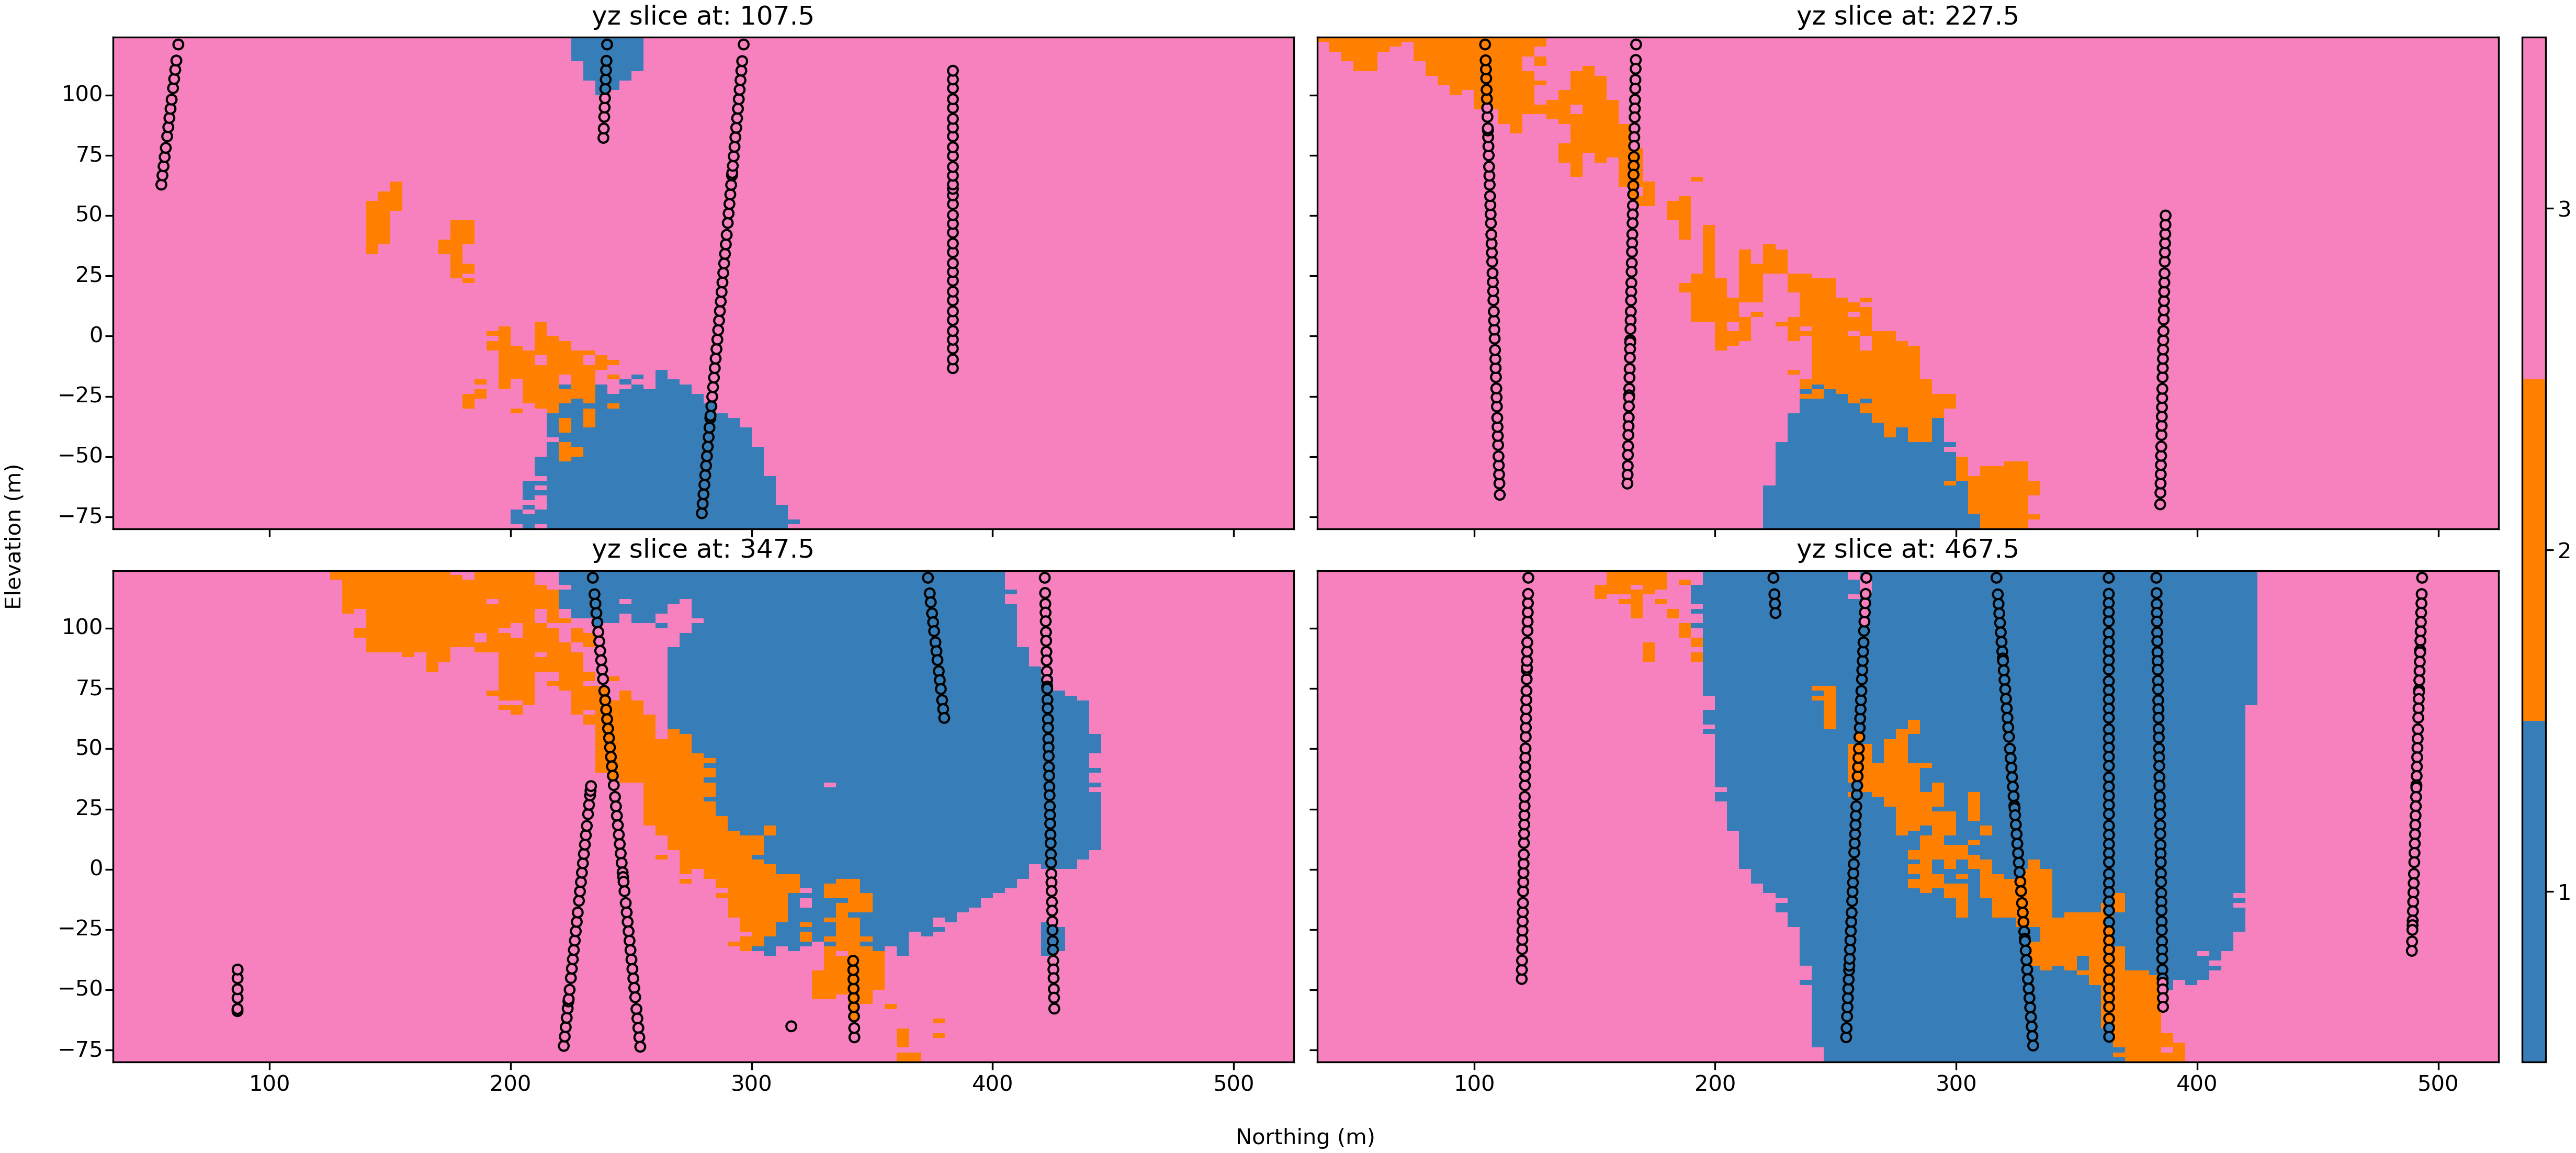
\includegraphics[width=0.5\textwidth]{capitulo_2/directsimreal1.png}\label{a}}
			\subfloat[][Realização 2]{\includegraphics[width=0.5\textwidth]{capitulo_2/directsimreal2.png}\label{b}}
	\end{figure}
\note{Esse slide mostra seções verticais de duas realizações do modelo. É possível observar nas regiões destacas bastante ruído, que gera formas não realistas. Além disso, em muitos casos, não existe um bom encaixe entre os blocos congelados e os blocos simulados. A simulação é muito sensível aos parâmetros e a zona de incerteza definida só serve pra dimuir o numero de blocos simulados, os limites dos modelos dependem somente dos parâmetros do algoritmo de simulação. 
	
	Porém o método trabalha com múltiplas categorias e é baseado em múltiplas realizações, o priduto final pode ser usado nas proximas etapas da avaliação de recursos e planejamento mineiro.}
\end{frame}

\begin{frame}{Simulação direta das distâncias assinaladas}
	\begin{enumerate}
		\item Cálculo das distâncias assinaladas para todas as amostras e categorias;
		\item Variografia das distâncias no espaço original para todas as categorias;
		\item Interpolação das distâncias; 
		\item criação do modelo com base na menor distância interpolada;
		\item Criação da zona de incerteza;
		\item Transformação Gaussiana das distâncias;
		\item Variografia das distâncias no espaço gaussiano para todas as categorias;
		\item Geração de múltiplos modelos baseados na menor distância simulada;
		\item Validação e pós processamento das realizações.
	\end{enumerate}
\note{Além das desvantagens apresentadas o método possui um número execivo de passos:
	
	As distancias devem ser calculadas pra cada litogia, variogradas e interpoaldas. Um modelo deterministico baseado na menor distancia deve ser criado, com base nas distancias interpoladas posso calcular o parametro u e definir a zona de incerteza, entao as distancias devem ser transfomradas para o espaco gaussiano, variografadas no espaco gaussiano, simuladas na zona de incerteza, retro transformadas e validadas. Aí sim posso gerar as realizações do modelo geológico baseadas na menor ditância simulada.
	
	É difícil justificar a escolha desse método.}
\end{frame}

\subsection{Simulação multi ponto}

\begin{frame}{Simulação multi ponto}

MPS em uma TI gerada pela interpolação das distâncias assinaladas.
	\begin{figure}[H]
		\caption{Diferentes realizações do modelo geológico.} 
		\label{snesim_real}
			\subfloat[][Realização 1]{\includegraphics[width=0.5\textwidth]{capitulo_2/snesim_real1.png}\label{a}}
			\subfloat[][Realização 2]{\includegraphics[width=0.5\textwidth]{capitulo_2/snesim_real2.png}\label{b}}
	\end{figure}
\note{Em sua tese de doutorado silva propôs integrar modelagem geológica implícita com simulação multi ponto. No seu trabalho ele propõe integrar múltiplas imagens de treinamento, uma metodologia pra calibrar a contribuição de cada TI e uma medida de entropia multi ponto ao longo dos furos. O esqueleto do método é criar uma TI a partir dos dados, que ele chama de data driven training image, usando funções distância assinaladas e aplicar MPS nessa TI.
	
	O slide mostra seções verticais de uma das realizações de um modelo criado usando essa metodologia no banco de dados do estudo de caso. As formas são geológicas, os modelos não apresentam ruído excessivo, além disso, o método não depende de muitos parâmetros. Em contra partida, não é possível definir uma zona de incerteza para que os contatos variem em seu interior, tampouco controlar a natureza dos contatos.}
\end{frame}

\subsection{Boundary simulation}

\begin{frame}{Boundary simulation}

Calibração do parâmetro C:

\begin{figure}[H]
	\caption{\label{c_param_1}Calibração do parâmetro C para a categoria 1.}
	\begin{center}
		\includegraphics[width=0.6\textwidth]{capitulo_2/uncert_1.png}
	\end{center}
	%\legend{Fonte: \citeonline{rolo_dissertacao}}
\end{figure}
\note{O próximo e último método, é o que produz os melhores resultados e o que tem sido mais usado pra avaliação de incerteza de modelos geológicos implíocitos. O primeiro passo é calibrar um parâmetro de incerteza de C. A calibração é feita por um método similar ao jacknife. 
	
	O parametro C é uma constante que vai ser somada às distâncias positivas e subtraído das distâncias negativas, isso faz com a diferença entre os valores das distâncias seja maior, é como se eu tivesse abrindo o histograma das distancias.
	
	Eu começo a calibração com c =0, então as distancias não estão modificadas ainda. Eu defino uma proporção de furos do banco de dados pra ser removida, pra categoria 1 do banco de dados do estudo de caso eu escolhi 25\%. Então eu removi do banco de dados, aleatoriamente, 25\% dos furos, 50 vezes, gerando 50 bancos de dados diferentes. Que são os pontos verticais no x=0. Então eu vou estimar a distância assinaladas onde eu removi as amostras, e checar se eu acerto se pertence ou não ao domínio, quer dizer se eu acerto o sinal da amostra, não estou interessado no valor da distância assinalada. Aí eu marco no eixo y, o índice de amostras classificadas de forma errada, pra cada um dos 50 banco de dados. 
	
	Então eu inceremento C, nesse exemplo o c variou de 0 ate 250, e repito o processo. quanto maior for C, menor vai ser o indice de classificação errônea.
	A partir dos resultados da calibração eu preciso escolher um valor de C. Alguns autores dizem que deve ser o valor reponsavel por 2,5\% de classificação errônea, outros autores dizem que deve ser o valor de C onde a curva se estabiliza. Aqui eu tomei o valor 130, que corresponde a 2\% de classificação errônea.}
\end{frame}

\begin{frame}{Boundary simulation}

	\begin{equation}
	d_k(u_\alpha)=\begin{cases}
	-\parallel u_\alpha-u_\beta\parallel - C,\:\textrm{se $u_\alpha$ pertence ao domínio}\\
	+\parallel u_\alpha-u_\beta\parallel + C,\:\textrm{se $u_\alpha$ não pertence ao domínio}\end{cases}
	\label{C_dist}
	\end{equation}
	
	Para que a simulação seja realizada de forma uniforme entre –C e +C, o desvio padrão $y`(u)$, deve ser simulado e transformado pela relação:
	
	
	\begin{equation}
	df'(u)=2*C*G^-1(y'(u))-C
	\end{equation}
	
	onde: $df'(u)$ é o valor da função distância simulada, $y'(u)$ o valor normal padrão da simulação não condicional, e $G^-1$ representa a determinação do valor da distribuição acumulada padrão normal correspondente a $y'(u)$. Para garantir que os valores pertençam a região estabelecida, os valores são multiplicados por 2C e subtraídos de C.
\note{A partir do valor escolhido para C, eu modifico as distâncias calculadas, somando C às distâncias positivas e subtraindo C das distâncias negativas.
	
	Então essas distâncias modificadas são interpoladas para todos os nós do grid, uma truncagem no modelo interpolado deve ser feita entra -c e +c pra definir a zona de incerteza.
	
	Na zona de incerteza eu realizao uma simulação gaussiana não condicional, o variograma pode ser o mesmo usado para interpolar as distâncias assinaladas. Para tornar a simulação gaussiana entre +c e -c deve ser tomado seu valor acumulado, multiplicado por 2c e subtraído de C.}
\end{frame}

\begin{frame}{Boundary simulation}

	Classificação dos blocos.

	\begin{figure}[H]
	\caption{\label{class}Classificação dos locais comparando valores estimados e simulados.}
	\begin{center}
		\includegraphics[width=0.7\textwidth]{capitulo_2/classificacao.png}
	\end{center}
	%\legend{Fonte: Modificado de \citeonline{wilde_sim_bound_reals}}
\end{figure}
\note{Agora finalmente eu posso classificar os blocos comparando as distâncias assinaladas modificadas com a simulação não condicional, blocos onde a simulação é menor que a interpolação não pertencem ao domínio enquanto blocos em que a simulação é maior que a interpolação, pertencem ao domínio.}
\end{frame}

\begin{frame}{Boundary simulation}
	\begin{figure}[H] 
		\caption{Interpolação, simulação e classificação na zona de incerteza.} \label{cat1_bound_sim}
		\centering
		\subfloat[][Distâncias interpoladas]{\includegraphics[width=.3\textwidth]{capitulo_2/interpolated.jpeg}\label{<figure1>}}
		\subfloat[][Distâncias simuladas]{\includegraphics[width=.3\textwidth]{capitulo_2/simulated.jpeg}\label{<figure2>}}
		\subfloat[][Classificação]{\includegraphics[width=.3\textwidth]{capitulo_2/classification.jpeg}\label{<figure2>}}
	\end{figure}
\note{Esse slide mostra as distâncias interpoladas na zona de incerteza para a categoria 1, as distancias simuladas na zona de incerteza, e os blocos classificados comparando ditancias intepoladas e simuladas.}
\end{frame}

\begin{frame}{Boundary simulation}

Blocos classificados.

	\begin{figure}[H]
		\caption{Seções verticais de uma realização para a categoria 1.} 
		\label{cpar_real}
			\subfloat[][Seção em XY]{\includegraphics[width=0.5\textwidth]{capitulo_2/cpar1.png}\label{a}}
			\subfloat[][Seção em YZ]{\includegraphics[width=0.5\textwidth]{capitulo_2/cparyz.png}\label{b}}
	\end{figure}
\note{O próximo slide mostra seções verticas em xy e xz de uma das realizações para a categoria 1. É possível observar que não há presença de ruído, as formas são suaves e realistas, além disso, ao contrário da simulação direta das distâncias, aqui o contato varia dentro da zona de incerteza, se a zona for larga a posição do contato e consequente o volume do solido vai ter grabnde variação, se for estrito terá pouca variação, o variograma controla a natureza do contato, um range maior produz contatos suaves enquanto ranges menores e efeito pepita produzem contatos rugosos. Apesar dessas vantagens a escolha do C pode ser subjetiva, e o método trabalha de forma binária, uma litologia por vez.}
\end{frame}

\subsubsection{Abordagem hierárquica}

\begin{frame}{Abordagem hierárquica}
	\begin{figure}[H]
		\caption{\label{hier_ex}Esquema do método mostrando os passos necessários.}
		\begin{center}
			\includegraphics[width=\textwidth]{capitulo_2/hier_example.png}
		\end{center}
		%\legend{Fonte: Modificado de \citeonline{amarante_incerteza_associada}}
	\end{figure}
\note{Aqui no laboratório nós desenvolvelmos uma metodologia pra trabalhar com múltiplas categorias simultânes de forma hierárquica, porém a escolha dos gruipos é subjetiva e depende de conhecimento a respeito da gênese do depósito.}
\end{frame}

\subsection{Sumário dos métodos de avaliação de incerteza}

\begin{frame}{Sumário dos métodos de avaliação de incerteza}
	

	\begin{table}[H]
		\centering
		\resizebox{\textwidth}{!}{
			\begin{tabular}{lcccccc}
				Método & \multicolumn{1}{l}{Simplicidade} & \multicolumn{1}{l}{Velocidade} & \multicolumn{1}{l}{Multi categórico} & \multicolumn{1}{l}{Realismo geológico} & \multicolumn{1}{l}{Controle da incerteza} & \multicolumn{1}{l}{Controle do tipo de contato} \\
				\midrule
				Heurístico & simples & rápido & sim   & não   & sim   & não \\
				Boundsim & simples & rápido & não   & sim   & não   & não \\
				Simulação direta & complexo & demorado & sim   & não   & sim   & não \\
				MPS   & simples & rápido & sim   & sim   & não   & não \\
				Boundary simulation & simples  & rápido & não   & sim   & sim   & sim \\
				\bottomrule
			\end{tabular}
		}
		%\caption{Sumário dos métodos de avaliação de incerteza de modelos geológicos.}\label{sumario}%
	\end{table}
\note{Essa tabela mostra um sumário dos métodos de avaliação de incerteza apresentados, o método heuristico é simple's, rápido, multi categorico, porem nao produz modelo com realismo geologico, mas controla a incerteza por meio do parametro gamma mas nao o tipo de contato.
	
	o metodo boundsim é simples, rapido, não trabalha com diferentes categorias, não apresenta realismo geologico, em tese seria possivel controlar a incerteza tomando diferentes valores para a media, mas isso nao acontece na pratica, também nao é possivel controlar o tipo de contato.
	
	A simulacao direta das distancias é um metodo complexo e demorado que trabalha com multiplas categorias simultaneamente porem nao apresenta realismo geologico nem permite o controle do tipo de contato, mas permite controlar a incerteza por meio dos parametros da simulacao.
	
	O metodo que mescla mps com modelagem implicita é simples rapido, multicategorico apresenta realismo geologico mas nao permite controlar a incerteza nem o tipo do contato.
	
	Finalmente o ultimo método, boundary simulation, é simples, rapido ja que a simulacao nao é condicional, nao é multi categorico mas apresenta realismo geologico, permite controle da incerteza e do tipo de contato. é o método que marca mais checkboxes disponivel na literatura.
	
	Isso encerra o estado da arte e os próximos slides tratam da minha proposta de tese}
\end{frame}

\section{Proposta de tese}

\subsection{Problemas}

\begin{frame}[allowframebreaks]{Problemas}

	\begin{itemize}
		\item Não estacionariedade da função distância assinalada torna a modelagem dos variogramas arbitrária e questionável;
		\item É preciso encontrar um balanço entre número de nós e resolução necessária. A resolução do \textit{grid} influencia diretamente a avaliação de incertezas;
		\item A escolha do interpolador muitas vezes é subjetiva e confusa;
		\item Na presença de múltiplos domínios, principalmente em ambientes geológicos complexos, é necessário a aplicação de uma lógica de precedência de estruturas ao invés de simplesmente tomar a menor distância assinalada para a criação de modelos realistas;
		\item Em alguns métodos a definição da zona de incerteza é subjetiva e não segue nenhuma regra matemática ou geológica, em outros a definição da zona de incerteza é extremamente laboriosa e complicada;
		\item Estruturas geológicas específicas, como lentes ou diques, podem desaparecer, ou não serem bem reproduzidas nos modelos implícitos;
		\item É necessário checar se os modelos implícitos honram a geologia do depósito e serão úteis para o processo de avaliação de recursos/reservas.
	\end{itemize}
\note{Embora a modelagem geoógica implícita seja um método consagrado que vem sendo usado com sucesso há mais de uma década, a metodologia apresenta alguns problemas pontuais:
	
	* o ponto mais critico, que todos os revisores de artigo questionam e é uma dificuldade prática pra quem usa método também é a não estacionariedade das distâncias, que torna a modelgaem do variograma questionável;
	
	* além disso, a escolha dos parametros do grid pode ser subjetiva;
	
	* Assim como a escolha do interpolaor;
	
	* Na presença de multiplos dominios, para geologias complexas, simplesemnte tomar a menor distância não produz bons resultados, é necessário uma abordagem hierárquica baseada na gênese do depósito;
	
	* Nos métodos de avaliação de incerteza que usam algum tipo de zona de incerteza, muitas vezes, essa zona não é de fato incerta, existem amotras dentro das zona;
	
	* Estruturas geológicas específicas, como lentes, diques, falhas, dobras, podem não ser reproduzida ou desaparecerem dos modelos;
	
	* é necessário checar se os modelos implítos honram a geologia do depósito e serão úteis nas fases seguntes do processo de avaliação de recursos.}
\end{frame}

\subsection{Interpolador}

\begin{frame}{Interpolador}

Redes neurais trabalham em um sistema binário de zeros e uns e por isso podem se basear nas propriedades da função sigmóide.

\begin{figure}[H]
	\caption{\label{nn_ex}Rede neural.}
	\begin{center}
		\includegraphics[width=0.7\textwidth]{capitulo_3/NN_ex.png}
	\end{center}
	%\legend{Fonte: \citeonline{samson_intro_ml}}
\end{figure}
\note{O primeiro aprimoramento que essa tese propões é um novo interpolador para as distâncias assinaladas. 
	
	Redes neurais são baseadas em neurônios, e usadas tipicmente em problemas de identificação.
	
	Esse slide esquematiza uma rede neural. Os nós x na camada um da rede representam os inputs, os nós a na camada dois e três representam as camadas escondidas e a camada 4 é o nó de output e representa a hipótese.
	
	As redes neurais trabalham em um sistema binário de zeros e uns e por isso podem se basear nas propriedades da função sigmoide, que tem seu valor em y entre zero e um para qualquer valor de x. Em uma rede neural uma hipótese é gerada para cada nó e é determinado se seu valor será zero ou um, um valor binário é passado para a próxima camada.}
\end{frame}

\begin{frame}{Interpolador}
	
	\cite{samson_estimation_ml} desenvolveram um algoritmo, usando TensorFlow.

	\begin{figure}[H] 
		\caption{Comparação de modelos gerados por diferentes métodos de estimativas.} \label{comparation}
		 \centering
		 \subfloat[][Realidade]{\includegraphics[width=.3\textwidth]{capitulo_3/actual.png}\label{<figure1>}}
		 \subfloat[][Estimativas por SK]{\includegraphics[width=.3\textwidth]{capitulo_3/krig.png}\label{<figure2>}}
		 \subfloat[][Estimativas por ML]{\includegraphics[width=.3\textwidth]{capitulo_3/ml.png}\label{<figure2>}}
		 %\legend{Fonte: \citeonline{samson_estimation_ml}}
	\end{figure}
	\note{Samson e deutsh propuseram um algoritmo usando tensor flow, que é uma biblioteca da google de código aberto para aprendizado de máquina, para implementar a arquitetura da rede neural. O método é baseado em aprendizado não supervisionado, com o algorito k means e supervisionado com uma rede neural de bases radiais.
		
		Redes neurais de bases radiais apresentam uma arquitetura semelhante as redes neurais artificais, a principal diferença é que nas redes neurais de bases radiais só há uma camada escondida e a função de ativação é uma função de base radial ao invés de uma função sigmoide.
		
		Em seu trabalho os autores dividiram o banco de dados em 2/3 para treinamento e 1/3 para teste. Usaram o algoritmo k-means pra determinar o numero de unidades de bases radiais na rede neural. A função de ativação alimentou o algoritmo com coordenadas x, y e z e teores das 5 amostras mais próximas do local a ser estimado.
		
		As imagens mostram mostram a realidade estimativas por krigagem simples e estimativas pelo metodo proposto, que reprodu as caracteristicas visuais da imagem de referencia bem como o variograma e histograma.
		
		Esse algoritmo resolve o problema do interpolador e do variograma ja que essa tecnica nao exige calculo e modelagem da covariância. A pesqusa de samsom e deutsch ainda está em seus estágios iniciais, els nao treinaram o parametro beta da funcao de base radial por exemplo. 
		
		Essa técnica tem um potencial enorme de aplicação na modelagem geológica implicita, porque evita a modelagem do variograma e a escolha de um interpolador. Além disso a função radial gaussiana já é a mais indicada e utilizada com sucesso na interpolação das distâncias. O método ainda pode evoluir para um algoritmo de simulação pra avaliar incerteza dos modelos gelógicos.}
\end{frame}

\subsection{Zona de incerteza}

\begin{frame}{Zona de incerteza}

	Gerar múltiplas realizações com a finalidade de avaliar a incerteza de modelos geológicos em todos os nós do \textit{grid} é desperdício de tempo e poder computacional, já que no interior dos domínios não há incerteza. 
	
	\begin{figure}[H] 
		\caption{Zonas de incerteza e contatos.} \label{zonas}
		\centering
		\subfloat[][Zona de incerteza 1]{\includegraphics[width=.4\textwidth]{capitulo_3/zona1.jpg}\label{zona1}}\qquad
		\subfloat[][Zona de incerteza 2]{\includegraphics[width=.4\textwidth]{capitulo_3/zona2.jpg}\label{zona2 2}}
	\end{figure}
\note{Um outro objetivo dessa tese é desenvolver uma metodologia objetiva e direta para a definição da zona de incerteza. Ás metodologias disponíveis na literatura podem gerar zonas de incerteza em interseçao com amostras.
	
	É necessário definir essas zonas de incerteza porque eu não preciso simular o grid inteiro, reduzindo o tempo e o esforço computacional e além disso, o método de avaliação de incerteza proposto nessa tese depende de diretamente da largura da zona de incerteza, os contatos variam em seu interior, zonas de incerteza maiores gera maior variação de volume dos corpos geológicos.
	}
\end{frame}

\begin{frame}{Zona de incerteza}
	Em física, a entropia é uma media do grau de desordem em um sistema.
	
	\begin{equation}
	H(X)=H(p_1, ..., p_n)=-\sum^n_{i=1}p_ilog_{2}p_i
	\end{equation}
	
	\begin{figure}[H] 
		\caption{Probabilidades de cada categoria em dois diferentes blocos.} \label{entro_block}
		\centering
		\subfloat[][Bloco 1]{\includegraphics[width=.4\textwidth]{capitulo_3/bloco1.jpg}\label{bloco1}}
		\subfloat[][Bloco 2]{\includegraphics[width=.4\textwidth]{capitulo_3/bloco2.jpg}\label{bloco 2}}
	\end{figure}
\note{A ideia central da metodologia proposta é a entropia, que é calculada como: menos o somatório do produto da probabilidade de cada de cada litologia pelo logaritmo da probabilidade. Dessa forma, a entropia pode ser vista como uma medida da incerteza. 
	
	suponha dois blocos e as probabilidades deles pertecerem a cada uma de três litologias, as probabilidades podem ser facilmente calculadas transformando distâncias estimadas em probabilidades, como mostrado no método heurístico de avaliação de incerteza. A entropia do primeiro bloco é baixa, já que a a categoria 1 tem probabilidade 80\% enquanro a entropia do bloco 2 é alta, porque todas as categorias têm probabilidades similares.}
\end{frame}

\begin{frame}{Zona de incerteza}
\begin{figure}[H]
	\caption{Entropias calculadas para diferentes valores de $\gamma$.} 
	\label{entro_gamma}
		\subfloat[][$\gamma=20$]{\includegraphics[width=0.5\textwidth]{capitulo_3/entropy_20.png}\label{a}}
		\subfloat[][$\gamma=10$]{\includegraphics[width=0.5\textwidth]{capitulo_3/entropy_10.png}\label{b}}
\end{figure}
\note{A transformação das distâncias em probabilidades envolve um paâmetro gamma, que contrala a incerteza, esse slide mostra duas seções verticais da entropia calculada para o banco de dados do estudo de caso, com dois valores de gamma diferentes. 
	
	O desafio é desenvolver uma metodologia para calibrar o parametro gamma, de forma que onde existam amostras a entropia seja máxima.
	
	depois de calcular a entropia, uma truncagem deve ser realizada para definição da zona de incerteza. Essa truncagem pode ser baseada no tipo de depósito, depositos com menor entropia de formação, como de bauxita, por exemplo, terão uma zona de incerteza mais estreita. enquanto depositos com alta entropia de formação, como os de ouro, terão zonas de incertezas mais largas.}
\end{frame}

\subsection{Avaliação da incerteza}

\subsubsection{Boundary simulation multi categórico}

\begin{frame}{Boundary simulation multi categórico}
	\begin{figure}[H]
		\caption{\label{comp_multi}Comparação multi categórica.}
		\begin{center}
			\includegraphics[width=0.8\textwidth]{capitulo_3/classificacao_multi.jpg}
		\end{center}
		%\legend{Fonte: \citeonline{samson_intro_ml}}
	\end{figure}
\note{Essa tese também propões investigar diferentes ténicas para a avaliação da incerteza em modelos geológico multi categóricos. Para que os modelos gerados sejam livres de ruído, tenham contatos suaves e contínuos e para que o que método seja rápido e não exija muito esforço computacional é preciso que esses métodos sejam baseados em uma variável auxiliar contínua, gerada por simulação não condicional. 
	
	O primeiro método que eu quero investigar é baseado no boundary simulation, que mostrei alguns slides atrás. A diferença aqui é que pra múltiplas categorias preciso de múltiplas distâncias simuladas que serão comparadas às estimadas ou será necessário estandardizar as distâncias interpoladas para que possam ser coparadas com uma única variável simulada.}
\end{frame}

\subsubsection{P-field}

\begin{frame}{P-field}
	Uma alternativa à simulação não condicional das distâncias na zona de incerteza são os campos de probabilidade (\textit{P-field}). A ideia central desse método de simulação é dissociar a tarefa de estimar distribuições de probabilidades locais para geração de múltiplas realizações equiprováveis \cite{froidevaux1993probability}. Uma premissa é de que as distribuições locais são conhecidas, o que é uma premissa razoável, já que as distribuições locais podem ser calculadas transformando distâncias em probabilidades.
	\note{Uma outra avenida que eu acredito que vale a pena ser investigada é o o p-field ou campos de probabilidade. Um campo gaussiano é gerado na zona de incerteza, a partir dos dos valor acumulado, eu posso amostrar uma distribição local de probabilidades,  bloco a bloco, que foi criada a partir da transformação das distâncias em probabilidades.}
\end{frame}

\subsubsection{Simulação plurigaussiana truncada}

\begin{frame}{Simulação plurigaussiana truncada}
	\begin{figure}[H]
		\caption{\label{trunc_gauss}Esquema da SGT. Note que as litologias sandstone e shale não aparecerão juntas nas realizações.}
		\begin{center}
			\includegraphics[width=0.5\textwidth]{capitulo_3/gauss_trunc_sketch.png}
		\end{center}
		%\legend{Fonte: \citeonline{deutsch2014multidimensional}}
	\end{figure}
\note{Ainda outra abordagem para a avaliação de incerteza que eu pretendo investigar é baseada em simulação plurigaussiana truncada. 
	
	Na simulação gaussiana truncada, uma variável continua gaussiana é simulada, e o histograma de cada realização é truncado em limites pré definidos para gerar uma variável categórica. 
	
	A imagem mostra a representação de um histograma de uma variável gaussiana, entao toda vez que o valor simulado para um bloco cair nessa regiao da esquerda ela é classificada como arenito, arenito-xisto na regiao central e xisto na região à direita.
	
	O uso de apenas uma variável gaussina pra derivar a variável categórica, em muitos casos é restritivo demais, porque limita a técnica ambientes estratificados, onde algumas das litogias não se tocam.}
\end{frame}

\begin{frame}{Simulação plurigaussiana truncada}
\begin{figure}[H]
	\caption{\label{trunc_pluri}Esquema da SPT. Note que as litologias 1 e 3 não aparecerão juntas nas realizações.}
	\begin{center}
		\includegraphics[width=0.5\textwidth]{capitulo_3/pluri_sketch.png}
	\end{center}
	%\legend{Fonte: \citeonline{deutsch2014multidimensional}}
\end{figure}
\note{Uma evolução natural da simulação gaussiana truncada, é a simulação pluri gaussiana truncda, que usa mais de uma variável gaussiana para derivar a variável categórica, permitindo a reprodução de estruturas mais complexas. Embora seja possível usar quantas variáveis gaussianas se desejar, o uso geralemtne é limitado à apenas duas, pela dificuldade em se criar regras de truncagem em mais de duas dimensões.
	
	Regra de truncagem é uma parte importante da metodologia, ja que ela controla os contatos entre as categorias, suas trabsições e proporções. A regra de truncagem, tradicionalemnte, é baseada nas probabilidades de transição calculadas a partir dos dados.
	
	Essa figura mostra duas variaveis gaussianas x e y, e uma regra de truncagem definida para quatro categorias, diferentemente da simulacao gaussiana truncada, eu preciso observar o valor das duas gaussianas simultaneamente, e a partir da regra de truncagem, classificar o bloco simulado. Entao se na gaussiana y o valor simulado caiu nessa regiao, e na gaussiana x, caiu nessa, por exemplo, o bloco é classificado como litologia 3.}
\end{frame}

\begin{frame}{Simulação plurigaussiana truncada}
	\begin{figure}[H]
		\caption{\label{trunc_rules}Diferentes templates, para o caso de duas variáveis latentes e quatro categorias.}
		\begin{center}
			\includegraphics[width=0.5\textwidth]{capitulo_3/trunc_rules.png}
		\end{center}
		%\legend{Fonte: Modificado de \citeonline{armstrong2011plurigaussian}}
	\end{figure}
\note{Diferentes regras de truncagem pode ser definidas, geralmente o espaço gaussiano multivariado é particionado em paralelepípedos, como os mostrados no slide, mas diferentes tecnicas para a regra de truncagem foram propostas:}
\end{frame}

\begin{frame}[allowframebreaks]{Regras de truncagem}
	\begin{itemize}
		\item \cite{allard2012non} introduziram o \textit{assignation diagram}, que automaticamente constrói a regra de truncagem para o caso bivariado usando regressão baseada em kernel em variáveis auxiliares;
		\item \cite{sadeghi_optimizing} usaram \textit{simulated annealing} para otimizar a regra de truncagem. A função objetivo é a minimização da classificação errônea entre as probabilidades de transição calculadas de realizações e das probabilidades de transição calculadas a partir dos dados.
		\item \cite{deutsch2014multidimensional} usaram \textit{multidimensional scaling} (MDS) para definir regras de truncagem complexas com o foco em reproduzir as probabilidades de transição. Essa metodologia pode ser aplicada para qualquer número de variáveis gaussianas.		 
		\item \cite{astrakova2015truncation} propuseram uma metodologia semelhante a de \cite{deutsch2014multidimensional} usando entropia bayesiana máxima em conjunto com \textit{simulated annealing} para otimizar a regra de truncagem bigaussiana;
		\item \cite{madani2015simulation} e \cite{hier_plurigauss} propuseram uma abordagem hierárquica para definir a regra de truncagem em espaços multi dimensionais.
\end{itemize}
\note{
	* Allard constroi automaticamente a regra de truncagem usando regressao baseada em kernel
	
	* sadeghi e boisvert usaram sikulated anealing para otimizar a regra de truncagem
	
	* deutch pai e dutsh filho usaram MDS pra definir regras de truncage complexas
	
	* astrakiva propos uma metodoloia semelhante a do deutsh
	
	* e finalmente o emery e o silva propuseram uma abordagem hierárquica pra definir a regra de truncagem}
\end{frame}

\begin{frame}{Regra dinâmica de truncagem}
\begin{figure}[H]
	\caption{\label{trunc_rules_prop}Diferentes regras de truncagem definidas para cada bloco a partir das probabilidades calibradas e calculadas.}
	\begin{center}
		\includegraphics[width=0.6\textwidth]{capitulo_3/trunc_rules_prop.jpg}
	\end{center}
	%\legend{Fonte: Modificado de \citeonline{armstrong2011plurigaussian}}
\end{figure}	
\note{Geralmente essas regras de truncagem são definidas globalemtne e usadas para todo o deposito, mas em muitos casos as proporções não são estacionárias matheron propos em 1987 curvas de proporções verticas, nesse caso, a regra de truncagem variava com a profundidade.
	
	Essa tese propõe a definição dinâmica da regra de truncagem, bivariada, pra cada bloco mas somente dentro da zona de incerteza. A regra de truncagem é contruída a partir das probabilidades locais, que foram derivadas a partir das distâncias estimadas. 
	
	O slide mostra dois blocos em duas regiões diferentes do depósito, dentro da zona de incertza. Entao pra esse bloco debaixo existe uma probabilidade alta dele pertence a categoria rosa, e uma probabilidade mais baixa de pertencer a azul, ja o bloco de cima, existe a probabilidade de pertencer as tres categorias, a partir dessas probabilidades eu posso construir uma regra de truncagem, simular duas gaussianas nao condicionais, comparar o valor das duas com a regra de truncagem e classificar o bloco em cada realização.}
\end{frame}

\begin{frame}{Regra de truncagem via MDS}
\begin{figure}[H]
	\caption{\label{pluri_mds}Esquema do uso de MDS para definição da regra de truncagem.}
	\begin{center}
		\includegraphics[width=0.4\textwidth]{capitulo_3/pluri_mds.png}
	\end{center}
	%\legend{Fonte: \citeonline{deutsch2014multidimensional}}
\end{figure}
\note{Essa regra de truncagem deve ser definida de forma automática pra cada bloco, uma das técnicas que eu acredito ser bastante promissora é a proposta por deutshc pai e deutsh filho, que constrói a regra de truncagem a partir de MDS e decomposição de voronoi.
	
	Um outro desafio é definir os variograms das variáveis gaussianas que controlam a continuidade dos domínios.}
\end{frame}

\subsection{Validação}

\begin{frame}{Validação}
	\begin{figure}[H]
		\caption{\label{blob}Modelo implícito ruim, com a presença de estruturas e formas indesejadas (\textit{"blobs"}).}
		\begin{center}
			\includegraphics[width=0.7\textwidth]{capitulo_3/blob.jpg}
		\end{center}
		%\legend{Fonte: \url{https://www.linkedin.com/pulse/implicit-modelling-disasters-making-part-1-ron-reid/}, acesso em junho de 2019}
	\end{figure}
\note{Finalmente, o ultimo aprimoramento proposto nessa tese é um método de validação de modelos geológicos implícitos. 
	
	O estatistico box diz que todos os modelos estão errados mas alguns são úteis. O jun cowan que é um dos precursores da modelagem implicita, hoje trabalha na leapfrog, é um grande critico da modelagem implicita, ele diz que a modelagm implicta cria modelos de forma fácil e rápida mas cria modelos ruins de forma facil e rápida. 
	
	A modelagem implicta tende a gerar estrutas esféricas ou em forma de salsicha ao redor dos furos, como essas mostradas no slide, que não são estruturas geológicas.   
	
	Minha proposta é desenvolver um algoritmo para chegagem visual automática de modelos geológicos implícitos, esse algoritmo deve reconhecer padrões indesejadas, que serão corrigidas com a alteração de parâmtros ou utilizando outros métodos.}
\end{frame}

\subsection{Sumário}

\begin{frame}{Sumário}
	Em suma, essa tese propõe desenvolver e investigar:


\begin{itemize}
	\item Um interpolador baseado em redes neurais independente de variograma para a variável distância assinalada;
	\item Uma metodologia para calibração e definição de uma zona de incerteza multi categórica estatisticamente justa, livre de viés e que seja de fato incerta;
	\begin{itemize}
		\item{Calibração do parâmetro $\gamma$;}
		\item{Truncagem no campo de entropia.}
	\end{itemize}
	\item Uma metodologia para avaliação da incerteza que gere múltiplas realizações de modelos geológicos multi categóricos dentro da zona de incerteza, sem ruído e com a possibilidade de controlar a natureza dos contatos.\
	\begin{itemize}
		\item{Definição de uma regra de truncagem local para cada bloco.}
		\item{Definição de um modelo de covariância para cada variável latente, que seja representativo.}
	\end{itemize}
	\item Uma metodologia para validação de modelos geológicos implícitos.
	\begin{itemize}
		\item{Identificação automática de estruturas indesejadas.}
	\end{itemize}
 
\end{itemize}
\note{Em suma essa tese propõe:
	
	* O desenvolvimento de um interpolador baseado em redes neurais que não depende de um variograma;
	
	* O desenvolvimento de uma metodologia para calibracão de uma zona de incerteza justa e livre de viés, pra isso é preciso calibrar o parametro gamma, usado na tranformação das distâncias em probabilidades e truncar o campo de entropia, com base no tipo de depósito;
	
	* uma metodologia para avaliação de incerteza que gere modelos continuos, livres de ruido, pra isso é preciso definir uma regra de truncagem local em cada bloco e definir um modelo de covariancia pra cada variavel latente, ou variavel gaussiana auxiliar.
	
	* e finalemtne uma metodologia pra validar modelos implícitos, que identifique de forma automatica padroes indesejáveis.}
\end{frame}

\subsection{Cronograma e atividades}

\begin{frame}{Progresso de desenvolvimento}
	\begin{itemize}

			\item Cálculo das distâncias assinaladas \checkmark
			\item Validação cruzada \checkmark
			\item Interpolação tradicional por RBF \checkmark
			\item Interpolação baseada em redes neurais
			\item Calibração do parâmetro $\gamma$ a partir das amostras \checkmark
			\item Calibração do parâmetro $\gamma$ (nova abordagem)
			\item Cálculo das probabilidades \checkmark
			\item Cálculo da entropia \checkmark
			\item Definição do \textit{cutt-off} no campo de entropia
			\item Simulação da variável contínua auxiliar
			\item Definição da regra de truncagem local
			\item Algoritmo de validação visual

	\end{itemize}
\note{Eu já venho desenvolvendo uma biblioteca de modelagem geológica implícita em python, tá no github, convido todos os colegas a testarem e editarem o código. Por enquanto ala calcula as distâncias, faz validação cruzada baseadas em k-folds, interpola por rbf, eu trabalhei numa primeira tentativa de calibrar o gamma a partir das moastras, mas não deu muito certo, então estou trabalhando em uma nova abordagem. A biblioteca ainda calcula as probabilidades, e calcula a entropia, por enquanto.}
\end{frame}

\begin{frame}{Cronograma}
	\begin{figure}[H]
		\caption{\label{cronograma}Cronograma de atividades.}
		\begin{center}
			\includegraphics[width=\textwidth]{capitulo_3/cronograma_novo.png}
		\end{center}
		%\legend{Fonte: \citeonline{samson_intro_ml}}
	\end{figure}
\note{Estou entrando no segundo ano de doutorado, a revisão biliográfica já foi feita, eu comecei a trabalhar no desenvolvimento de software, no momento estou trabalhando na definição da zona de incerza, e dando os primeiros passos nas metodologias de avaliação de incerteza, para os proximoms meses o planejamento é também começar a trabalhar no interpolador. Os últimos meses serão dedicados à escrita da tese e publicação dos resultados.}
\end{frame}

%Referencias

\section{Referências bibliográficas}

\begin{frame}[allowframebreaks]{Referências bibliográficas}
	\bibliographystyle{apa}
	\bibliography{bibliografia}
	\note{Por fim as referências bibliográficas e eu gostaria de agradecer novamente a preseça de todos, ao LPM e à capes. Muito obrigado!}
\end{frame}

\end{document}